% ********************************************************************** %
% Dissertation template and document class for Princeton University      %
% Author  : Jeffrey Scott Dwoskin <jdwoskin@princeton.edu>               %
% Adapted from: http://www.math.princeton.edu/graduate/tex/puthesis.html %
% ********************************************************************** %

%%% For print copies
%% set 'singlespace' option to set entire thesis to single space, and define "\printmode" to remove all hyperlinks for printed copies of the thesis.
%% Delete all output files before changing this mode -- it will turn hyperref package on and off
%\documentclass[12pt,lot, lof, singlespace]{puthesis}
%\newcommand{\printmode}{}

%%% For the electronic copy, use doublespacing, define "\proquestmode" to use outlined links, instead of colored links. 
\documentclass[12pt,lot,lof]{puthesis} % 06/06/2017 jklew: MAKE SURE TO UNCOMMENT FOR FINAL VERSION
\newcommand{\proquestmode}{}
% I prefer proquestmode to be off for electronic copies for normal use, since the colored links are less distracting. However when printed in black and white, the colored links are difficult to read. 

%%% For early drafts without some of the frontmatter
% Also see the "ifodd" command below to disable more frontmatter
%\documentclass[12pt]{puthesis}

%%%%%%%%%%%%%%%%%%%%%%%%%%%%%%%%%%%%%%%%%%%%%%%%%%%%%%%%%%%%%\
%%%% Author & title page info

\title{Soot Modeling in Large Eddy Simulation of Turbulent Nonpremixed Combustion}

\submitted{September 2017}  % degree conferral date (January, April, June, September, or November)
\copyrightyear{2017}  % year in which the copyright is secured by publication of the dissertation.
\author{Jeffry Kimura Lew}
\adviser{Professor Michael E. Mueller}  %replace with the full name of your adviser
%\departmentprefix{Program in}  % defaults to "Department of", but programs need to change this.
\department{Mechanical and Aerospace Engineering}

%%%%%%%%%%%%%%%%%%%%%%%%%%%%%%%%%%%%%%%%%%%%%%%%%%%%%%%%%%%%%\
%%%% Tweak float placements
% From: http://mintaka.sdsu.edu/GF/bibliog/latex/floats.html "Controlling LaTeX Floats"
% and based on: http://www.tex.ac.uk/cgi-bin/texfaq2html?label=floats
% LaTeX defaults listed at: http://people.cs.uu.nl/piet/floats/node1.html

% Alter some LaTeX defaults for better treatment of figures:
    % See p.105 of "TeX Unbound" for suggested values.
    % See pp. 199-200 of Lamport's "LaTeX" book for details.
    %   General parameters, for ALL pages:
    \renewcommand{\topfraction}{0.85}	% max fraction of floats at top
    \renewcommand{\bottomfraction}{0.6}	% max fraction of floats at bottom
    %   Parameters for TEXT pages (not float pages):
    \setcounter{topnumber}{2}
    \setcounter{bottomnumber}{2}
    \setcounter{totalnumber}{4}     % 2 may work better
    \setcounter{dbltopnumber}{2}    % for 2-column pages
    \renewcommand{\dbltopfraction}{0.66}	% fit big float above 2-col. text
    \renewcommand{\textfraction}{0.15}	% allow minimal text w. figs
    %   Parameters for FLOAT pages (not text pages):
    \renewcommand{\floatpagefraction}{0.66}	% require fuller float pages
	% N.B.: floatpagefraction MUST be less than topfraction !!
    \renewcommand{\dblfloatpagefraction}{0.66}	% require fuller float pages

% The documentclass already sets parameters to make a high penalty for widows and orphans. 

%%%%%%%%%%%%%%%%%%%%%%%%%%%%%%%%%%%%%%%%%%%%%%%%%%%%%%%%%%%%%\
%%%% Use packages

%\usepackage{amsfonts}

% Proper font encoding, especially for dashes in bibliography
\usepackage[english]{babel}
\usepackage[utf8]{inputenc}
\usepackage[T1]{fontenc}

% To allow for text in math mode
\usepackage{amsmath}

% For bold math text
\usepackage{bm}

%%% For figures
\usepackage{graphicx}
%\usepackage{subfig,rotate}

%%% for comments
\usepackage{verbatim}

%%% For tables
\usepackage{multirow}
% Longtable lets you have tables that span multiple pages.
\usepackage{longtable}

% Booktabs produces far nicer tables than the standard LaTeX tables.
%   see: http://en.wikibooks.org/wiki/LaTeX/Tables
\usepackage{booktabs}

%set parameters for longtable:
% default caption width is 4in for longtable, but wider for normal tables
\setlength{\LTcapwidth}{\textwidth}

% So citations are in numerical order and grouped together if possible (i.e., 3-5 instead of 3,4,5)
\usepackage{cite}

% For the degrees symbol
\usepackage{textcomp,gensymb}

% To write chemical reactions easily
\usepackage[version=4]{mhchem}

% For extra wide tildes
\usepackage{yhmath}

%%%%%%%%%%%%%%%%%%%%%%%%%%%%%%%%%%%%%%%%%%%%%%%%%%%%%%%%%%
%%% Printed vs. online formatting
\ifdefined\printmode

% Printed copy
% url package understands urls (with proper line-breaks) without hyperlinking them
\usepackage{url}


\else

\ifdefined\proquestmode
%ProQuest copy -- http://www.princeton.edu/~mudd/thesis/Submissionguide.pdf

% ProQuest requires a double spaced version (set previously). They will take an electronic copy, so we want links in the pdf, but also copies may be printed or made into microfilm in black and white, so we want outlined links instead of colored links.
\usepackage{hyperref}
\hypersetup{bookmarksnumbered}

% copy the already-set title and author to use in the pdf properties
\makeatletter
\hypersetup{pdftitle=\@title,pdfauthor=\@author}
\makeatother

\else
% Online copy

% adds internal linked references, pdf bookmarks, etc

% turn all references and citations into hyperlinks:
%  -- not for printed copies
% -- automatically includes url package
% options:
%   colorlinks makes links by coloring the text instead of putting a rectangle around the text.
\usepackage{hyperref}
\hypersetup{colorlinks,bookmarksnumbered}

% copy the already-set title and author to use in the pdf properties
\makeatletter
\hypersetup{pdftitle=\@title,pdfauthor=\@author}
\makeatother

% make the page number rather than the text be the link for ToC entries
%\hypersetup{linktocpage}
\fi % proquest or online formatting
\fi % printed or online formatting

% For grouped references to equations
% Needs to be placed last, after all ``\usepackage'' commands
\usepackage[capitalise]{cleveref}


%%%%%%%%%%%%%%%%%%%%%%%%%%%%%%%%%%%%%%%%%%%%%%%%%%%%%%%%%%%%%\
%%%% Define commands

% Define any custom commands that you want to use.
% For example, highlight notes for future edits to the thesis
%\newcommand{\todo}[1]{\textbf{\emph{TODO:}#1}}

  %% Commands for writing equations
  \newcommand*\mc[1]{\mathcal{#1}}                % To change argument to script font
  \newcommand*\mean[1]{\overline{#1}}             % Average qtys. or LES low-pass filter
  \newcommand*\tf[1]{\widetilde{#1}}              % Density-weighted filter (LES low-pass filtered qtys.)
  \newcommand{\tff}[1]{\widetilde{\overline{#1}}} % Combine above two 
  \newcommand{\pder}[2][]{\frac{\partial#1}{\partial#2}}            % Partial derivative
  \newcommand{\sder}[2][]{\frac{\partial^{2}#1}{\partial#2^{2}}}      % Second partial derivative
  \newcommand{\tder}[1]{\pder[#1]{t} + \pder[u_j#1]{x_j}}            % Total derivative
  \newcommand{\trder}[1]{\pder[\rho #1]{t} + \pder[\rho u_j#1]{x_j}} % Total derivative (conservative form)

  % Density-weighted LES filtered total derivative (conservative form)
  \newcommand{\ftrder}[1]{\pder[\mean{\rho}#1]{t} + \pder[\mean{\rho}\tf{u}_j#1]{x_j}}

  % Divergence of subfilter flux
  \newcommand{\dsff}[2][]{\pder[]{x_j}\left( \mean{\rho}\tf{u}_j#1 - \mean{\rho}#2 \right)}

  % Density-weighted LES filtered diffusion term
  \newcommand{\fdt}[2][]{\pder[]{x_j}\left( \mean{\rho}\tf{D}_{#1}\pder[#2]{x_j} \right)}

  % LES filtered source term
  \newcommand{\fst}[2][]{\mean{\dot{#1}}_{#2}}

  % Modified script G in Presumed PDF section of Ch. 2
  \newcommand{\mg}[0]{\mc{G}^{\heartsuit}}
  

% create an environment that will indent text
% see: http://latex.computersci.org/Reference/ListEnvironments
% 	\raggedright makes them left aligned instead of justified
\newenvironment{indenttext}{
    \begin{list}{}{ \itemsep 0in \itemindent 0in
    \labelsep 0in \labelwidth 0in
    \listparindent 0in
    \topsep 0in \partopsep 0in \parskip 0in \parsep 0in
    \leftmargin 1em \rightmargin 0in
    \raggedright
    }
    \item
  }
  {\end{list}}

% another environment that's an indented list, with no spaces between items -- if we want multiple items/lines. Useful in tables. Use \item inside the environment.
% 	\raggedright makes them left aligned instead of justified
\newenvironment{indentlist}{
    \begin{list}{}{ \itemsep 0in \itemindent 0in
    \labelsep 0in \labelwidth 0in
    \listparindent 0in
    \topsep 0in \partopsep 0in \parskip 0in \parsep 0in
    \leftmargin 1em \rightmargin 0in
    \raggedright
    }

  }
  {\end{list}}

%%%%%%%%%%%%%%%%%%%%%%%%%%%%%%%%%%%%%%%%%%%%%%%%%%%%%%%%%%%%%\
%%%% Front-matter

% For early drafts, you may want to disable some of the frontmatter. Simply change this to "\ifodd 1" to do so.
\ifodd 1 % 06/06/2017 jklew: DEFAULT IS 0
% front-matter disabled while writing chapters
%%%\renewcommand{\maketitlepage}{}
\renewcommand*{\makecopyrightpage}{}
\renewcommand*{\makeabstract}{}

% you can just skip the \acknowledgements and \dedication commands to leave out these sections.

\else

% 06/21/2017 DEFAULT FOR BELOW IS UNCOMMENTED
\abstract{
% Abstract can be any length, but should be max 350 words for a Dissertation for ProQuest's print indicies (150 words for a Master's Thesis) or it will be truncated for those uses.
This is a test of the abstract.

%% This is a \LaTeX{} template and document class for Ph.D. dissertations at Princeton University. It was created in 2010 by Jeffrey Dwoskin, and adapted from a template provided by the math department. Their original version is available at: \url{http://www.math.princeton.edu/graduate/tex/puthesis.html}

%% This is \textbf{NOT} an official document. Please verify the current Mudd Library dissertation requirements~\cite{mudd2009} and any department-specific requirements before using this template or document class.


%% Your abstract can be any length, but should be a maximum of 350 words for a Dissertation for ProQuest's print indicies (or 150 words for a Master's Thesis); otherwise it will be truncated for those uses~\cite{proquest2006}.


%% Dwoskin Ph.D. Dissertation Template --- version 1.0, 5/19/2010

}

\acknowledgements{
%I would like to thank...
This thesis would not exist without the support I have received from people in the Princeton community and beyond. I am indebted to my advisor, Professor Michael E. Mueller, for his generosity with guidance and encouragement. I thank him for the myriad of ways he has contributed to my intellectual and professional growth.

I am beholden to my graduate student peers and Professors Elie Bou-Zeid, Luigi Martinelli, and Howard A. Stone for assisting me with general exam preparations. I thank Professors Marcus Hultmark, Yiguang Ju, Chung K. Law, and Alexander Smits for being my examiners. I would also like to express my gratitude to my advisor and Professor Yiguang Ju for serving as my reading committee.

Many aspects of this thesis would not have come to fruition without the cooperation of various outstanding researchers outside Princeton University. I am fortunate to have collaborated with Professor Antonio Attili and Mr. Lukas K. W. Berger at RWTH Aachen University and the following researchers at the University of Adelaide: Mr. Saleh Mahmoud, Professor Zeyad T. Alwahabi, Professor Bassam B. Dally, and Professor Graham J. Nathan.

I am grateful for the companionship of my colleagues in CTRFL: Dr. Temistocle Grenga, Dr. Suo Yang, Dr. Carla Bahri, Dr. Sili Deng, Jonathan F. MacArt, A. Cody Nunno, Sandra Sowah, Bruce A. Perry, and Alex G. Novoselov. The discussions that I had with them helped me overcome obstacles in my research, and their presence in lab reminded me that it is always sunny in D101.

I extend my appreciation to Seongwoo Oh, Justin L. Ripley, Jonathan Shi, and James E. Park for being compassionate cohabitants, and I am thankful for the Big Red comradeship of Seongwoo Oh, Zhaoqi Leng, Anthony Savas, and Daniel Floryan. Finally, I deeply thank my parents for their steadfast encouragement and support.

This work would not be possible without the valuable support in the form of computational time on the TIGRESS high performance computer center at Princeton University, which is jointly supported by the Princeton Institute for Computational Science and Engineering (PICSciE) and the Princeton University Office of Information Technology's Research Computing Department. This thesis carries T-3342 in the records of the Department of Mechanical and Aerospace Engineering.

%% Advisor
%% Thesis committee/generals committee
%% Professors who helped me during the general exam process
%% labmates + other labs + classmates + Daniel floryan
%% Jill Ray and Theresa
%% Susanne Killian
%% Roommates Seong, Justin
%% Ian, Bryan, going to the gym
%% Collaborators such as Bassam Dally
%% Susanne Killian and Shalin Shah
%% Advisors from Cornell (Olivier Desjardins, Elizabeth Fisher, Dr. Brandon Hencey)
%% Parents

%% I would like to thank the Math department for providing the original documentclass file that this class is based upon. I would like to thank my parents, without whom my life would not be possible. I would also like to thank my advisor, my dissertation committee, and my research collaborators because every graduate student needs to do so. And finally, I thank the members of my research group, to whom I leave this template to save you some of the trouble I had to go through getting my dissertation to compile in \LaTeX{}.  

%% Don't forget to ask your advisor if your work was sponsored by a grant that needs to be acknowledged in this section.

%% Lastly, I want to thank my parents for their 

}

\dedication{To my parents.}

\fi  % disable frontmatter


%%%%%%%%%%%%%%%%%%%%%%%%%%%%%%%%%%%%%%%%%%%%%%%%%%%%%%%%%%%%%\
%%%% Hide some chapters

%%% If you want to produce a pdf that includes only certain chapters, specify them with includeonly, in addition to including all chapters below.
%\includeonly{ch-intro/chapter-intro}
%%% You can also specify multiple chapters.
%\includeonly{ch-intro/chapter-intro,ch-usage/chapter-usage}
%\includeonly{chap1,chap2,chap3}

%\includeonly{ch-lesmodels/chapter-lesmodels}


%%%%%%%%%%%%%%%%%%%%%%%%%%%%%%%%%%%%%%%%%%%%%%%%%%%%%%%%%%%%%
%%%% Notes:

% Footnotes should be placed after punctuation.\footnote{place here.}
% Generally, place citations before the period~\cite{anotherauthor}.
% The proper usage for i.e., and e.g., include commas ``(e.g., option A, option B)''

%%%%%%%%%%%%%%%%%%%%%%%%%%%%%%%%%%%%%%%%%%%%%%%%%%%%%%%%%%%%%
%%%% Import chapters

\begin{document}

\makefrontmatter


% If you've disabled frontmatter, you can insert the toc manually
%\tableofcontents\clearpage % 06/06/2017 jklew: DEFAULT IS COMMENTED OUT

% \include lets us split up the document (and each include starts a new page):
\chapter{Introduction\label{ch:intro}}
 
Soot is a carbonaceous product formed from the incomplete combustion of hydrocarbon fuels. Although soot may appear as a dark cloud or plume to the naked eye, it is actually a collection of nanoscale particles, as shown in \cref{fig:intro:dieselsoot}. Soot particles are required to increase the radiant energy of flames in furnaces and boilers, but they are also an undesired waste product in many engineering systems such as internal combustion engines, gas turbine combustors, and combustion-based power plants. If released into the atmosphere, soot can contribute to haze, acid rain, and climate change. Exposure to these particles results in an increased risk for a variety of ailments including strokes~\cite{popeiii2006}, atherosclerosis~\cite{polichetti2009,kennedy2007,popeiii2006}, lung cancer~\cite{kennedy2007,popeiii2006}, and cardiovascular mortality~\cite{polichetti2009,kennedy2007,popeiii2006}, and these adverse health effects have been observed to be closely related the number, composition, and size of particles rather than their mass~\cite{seaton1995,lighty2000}. In many nations, regulations for particulate matter are expected to become more stringent in the coming decades.
% While the fate of federal regulations for particulate matter under the current administration of President Donald J. Trump is unclear, these regulations are expected to become more stringent in the coming decades. 

\begin{figure}[htb]
  \centering
  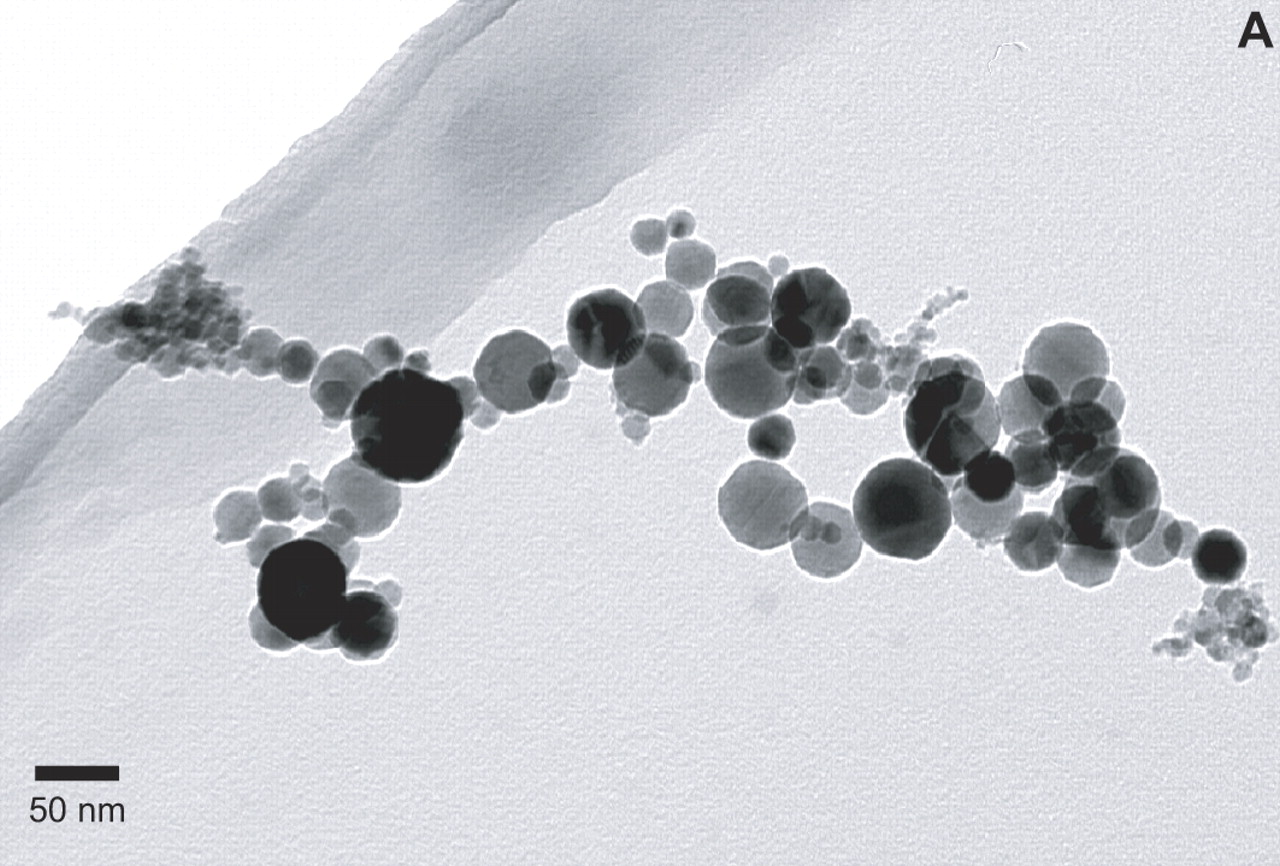
\includegraphics[width=0.4\linewidth]{ch-intro/figures/diesel-soot}
  \caption[Soot From a Diesel Car Engine]{Transmission Electron Microscope (TEM) image of soot collected from the exhaust of a diesel car engine. Reproduced from Grob\'ety \etal~\cite{grobety2010}.}
  \label{fig:intro:dieselsoot}
\end{figure}

The production of next-generation, environmentally friendly combustion systems will depend on numerical simulation for rapid design optimization. The task of predicting how soot evolves in the turbulent reacting flows of these systems is nontrivial and will require high-fidelity models for soot, combustion, and turbulence. The large range of spatial and temporal scales present in these systems makes the development of each component model extremely challenging. Furthermore, integration into a single framework necessitates accounting for the interactions between models. The preferred framework to design these low emissions systems is Large Eddy Simulation (LES), a computationally efficient approach where the large, geometry-dependent scales of the system are resolved and the small scales are modeled. Today's state-of-the-art simulations have progressed towards achieving this goal, but significant work still lies ahead.

The overall objective of this thesis is to advance the understanding of how turbulence affects the dynamics of soot. Specifically, the small-scale interactions between soot, chemistry, and turbulence as well as the transport of species in turbulent nonpremixed combustion are analyzed. The insights that are gained are used to develop models for LES. A survey of previous investigations on both topics is presented in the upcoming sections, but, first, a brief overview of the processes that guide the evolution of soot is provided.


%% ***
%% My rough idea for intro:
%% What is soot and why it needs to be studied/modeled
%% Explanation of dynamics of soot/various modes of evolution

%% Goal is to motivate need for ZASSP (closure model for soot transport equation SOOT MODEL that accounts for spatial intermittency of soot (soot-turbulence interactions) as well as its interaction/connection to combustion chemistry). Also need to motivate need for SSTA (transport approach that uses the nonpremixed flamelet framework TURBULENT COMBUSTION MODEL WITH EMPHASIS ON SOOT PRECURSORS with differential diffusion, transporting species with relatively slow chemistry with molecular diffusion and species with fast chemistry with unity effective Lewis numbers).

%% SOOT-TURBULENCE-CHEMISTRY INTERACTIONS:
%% Effects of turbulence on soot, experimental evidence of influence of strain
%% Previous modeling attempts of soot evolution in turbulent combustion: RANS, LES, DNS (highlight findings and weaknesses)
%% Explain how the model I developed will address these deficiencies

%% EFFECT OF TRANSPORT ON SOOT EVOLUTION:
%% Mention species that influence soot evolution and dictate flame structure have a variety of molecular weights and scales.
%% Somehow incorporate experimental findings into this section
%% Previous modeling attempts for transport of species in turbulent combustion (highlight findings and weaknesses, especially with consideration of soot)
%% Explain how the turbulent combustion transport model will address these deficiencies
%% ***

\section{Dynamics of Soot}
\label{sec:intro:dynamics}
%\section{Modeling Framework for Large Eddy Simulation}
%\label{sec:intro:framework}

%% Summarize previous works on soot and turbulent combustion models as well as other closure approaches other than the presumed PDF approach.

%% There are three classes of statistical models that are generally utilized. The most accurate is the Monte Carlo (MC) approach, where a large population of notional particles is used to represent the NDF. The evolution of these particles is determined by assuming that all aerosol processes are governed by stochastic processes~\cite{balthasar2003} or that only the coagulation of particles occurs stochastically~\cite{lucchesi2017}. MC is able to capture the NDF with high accuracy, as thousands of internal coordinates can be used to provide highly detailed descriptions of aggregate structure and chemical composition~\cite{celnik2008,mosbach2009}. However, the computational cost associated with such accuracy constrains the application of MC to simple configurations such as homogeneous reactors~\cite{celnik2007} and one-dimensional laminar premixed flames~\cite{patterson2007}. Additionally, explicitly coupling MC to the gas-phase chemistry is not straightforward~\cite{celnik2007}.

%% The second class of statistical models comprises sectional methods, where the NDF is discretized into bins and equations are solved for the number of particles in each bin. Like MC simulations, sectional methods provide accurate depictions of the complete NDF. However, as the number of internal coordinates used to describe the NDF increases, the associated computational cost can become intractable due to the required number of bins~\cite{gelbard1980}. Sectional methods do possess an advantage over MC, as they are deterministic and can be explicitly coupled to gas-phase chemistry.

The life of a soot particle begins with the formation of Polycyclic Aromatic Hydrocarbons (PAH). The exact mechanism for this process is not yet fully understood, but in general, large aliphatic fuel molecules are oxidized into smaller hydrocarbons by $\beta$-scission and \ce{H}-abstraction~\cite{law2006}. Further reactions eventually lead to the creation of species such as acetylene (\ce{C2H2}), propargyl (\ce{C3H3}), cyclopentadienyl (\ce{C5H5}), phenyl (\ce{C6H5}), and benzene (\ce{C6H6})~\cite{wang1997,richter2000,wang2011}. Benzene, the first aromatic ring, plays an important role in the production of multi-ring aromatic species. Larger PAH with molecular weights of 500-1000 amu are considered to be the immediate precursors of soot, and their formation can occur through the attachment of \ce{C2}, \ce{C3}, and other small units to benzene~\cite{wang1997,richter2000}. Growth is further fostered through the addition of PAH radicals and through reactions between PAH species, including PAH-PAH radical recombination and addition reactions~\cite{richter2000,wang2011}. Collisions between these gas-phase PAH lead to dimerization, and the collisions between PAH dimers form solid-phase nascent soot particles known as primary particles~\cite{frenklach1991,richter2000,schuetz2002,blanquart2009,wang2011}. This process can take several milliseconds~\cite{richter2000,wang2011} and is summarized in the first two frames of \cref{fig:intro:dynamics:sootdynamics}.

\begin{figure}[htb]
  \centering
  \includegraphics[width=\linewidth]{ch-intro/figures/soot-dynamics}
  \caption[Dynamics of Soot]{Various processes that govern the dynamics of soot.}
  \label{fig:intro:dynamics:sootdynamics}
\end{figure}

Once the first primary particles appear, their evolution is dictated by various physical and chemical processes. In the top right frame of \cref{fig:intro:dynamics:sootdynamics}, coagulation is depicted. During coagulation, the number density of particles decreases as existing particles collide and no mass is transferred from gas-phase species to solid-phase particles~\cite{kazakov1995,hmom2009}. There are two limits as to how coagulation can occur. In the limit of pure coalescence, a primary particle is assumed to undergo maximum deformation as it collides with another particle to form a larger spherical particle. This is facilitated by the liquid-like nature of nascent particles as noted in experimental studies~\cite{dobbins1998,dobbins2002}. In the limit of pure aggregation, the colliding particles do not deform and the total surface area is assumed to be preserved in the resulting particle.

Soot can also evolve through two different growth pathways, as shown in the bottom left and middle frames of \cref{fig:intro:dynamics:sootdynamics}. During condensation, a gas-phase PAH dimer collides with a soot particle and attaches to its surface~\cite{hmom2009,blanquart2009}. Surface growth, on the other hand, involves reactions with gas-phase acetylene. Carbon atoms are added to the surface of the soot particle through the \ce{H}-Abstraction \ce{C2H2}-Addition (HACA) mechanism~\cite{frenklach1985,frenklach1991}. Both growth processes influence soot morphology by rendering particles and aggregates more spherical~\cite{mitchell1998,mitchell2003,park2003}.

These growth modes are balanced by destructive modes, as illustrated in the bottom right frame of \cref{fig:intro:dynamics:sootdynamics}. Oxidation occurs when hydroxyl radicals (and molecular oxygen to a lesser extent) strip carbon atoms from the surfaces of soot particles, forming products such as \ce{CO} and \ce{CO2}~\cite{kazakov1995,neoh1981,stanmore2001}. Oxidation by hydroxyl radicals proceeds rapidly, but oxidation by molecular oxygen occurs slowly enough such that the internal structures of large aggregates are weakened. This leaves these aggregates susceptible to breaking apart in a process known as fragmentation~\cite{mueller2011,neoh1985}.

Clearly, the lifetime of soot is governed by interactions with species of various weights, length scales, and time scales. Accurately predicting the evolution of soot in a turbulent reacting flow requires accounting for these interactions as well as for the influence of the surrounding flow field. Previous research addressing these topics is surveyed in the upcoming sections.

\section{Soot-Chemistry-Turbulence Interactions}
\label{sec:intro:scti}

Discussion of previous works on subfilter modeling with respect to soot. Can discuss Monte Carlo approach, various method of moment approaches, etc.

\section{Effect of Transport on Soot Evolution}
\label{sec:intro:transport}

Can discuss various approaches to modeling transport for sooting flames. Can discuss diffusion between soot and gas-phase species (DNS paper by Jackie Chen).

Main points:
Discussion about soot PAH precursors and other strain-sensitive species.
Classical theory is that turbulence mixes indiscriminately at sufficiently high Re.
PAH are very sensitive to the local scalar dissipation rate due to their slow formation chemistry
DNS studies suggest PAH are confined to spatially intermittent regions of low scalar dissipation rate that are on the order of the Kolmogorov scale or smaller
At such scales, transport is governed by molecular diffusion
Pitsch and Peters flamelet equations with full differential diffusion
Wang's bimodal transport

\section{Organization of Thesis}
\label{sec:intro:org}

This thesis is organized as follows. In \cref{ch:lesmodels}, the foundation for modeling soot in LES of turbulent nonpremixed combustion is presented. In \cref{ch:subfilter}, the model for small-scale interactions between soot, combustion chemistry, and turbulence is developed and validated \textit{a priori} against a recent DNS database. In \cref{ch:transport}, the transport model for species with relatively slow formation chemistry is presented and validated \textit{a priori} with solutions to the flamelet equations. In \cref{ch:lesresults}, these models are implemented in LES and validated against experimental measurements from a series of three laboratory-scale flames. Finally, in \cref{ch:conclusion}, the results from this thesis are summarized and suggestions for future work are proposed.

The accomplishments and new contributions of this thesis are summarized below.
\begin{itemize}
\item \textbf{$Z$-Activated Soot Subfilter PDF (ZASSP):} Developed a presumed subfilter PDF model to close the filtered transport equations for the soot model. It contains a dependence on the mixture fraction to address the lack of soot in fuel-lean regions and has the form of a double-delta distribution to account for the high spatial intermittency of soot (Chapter 3).
\item \textbf{Strain-Sensitive Transport Approach (SSTA):} Developed a model that transports species governed by relatively slow formation chemistry with molecular diffusion and transports species governed by fast kinetics with equal effective diffusivities. A strain-sensitivity parameter is used to categorize each species (Chapter 4).
\item \textbf{Validation of the Integrated Large Eddy Simulation Model:} Conducted Large Eddy Simulations with ZASSP and SSTA for a series of three laboratory-scale ethylene-hydrogen-nitrogen simple jet flames (Chapter 5).
\end{itemize}



%% This documentclass, \texttt{puthesis.cls}, is setup for a Ph.D. dissertation for Princeton University. The Mudd Library website~\cite{mudd2009} provides detailed specifications for how to format your disseration~\cite{muddthesis2009}. Please review those documents, as the requirements may have changed since this template was created. Also, review the ProQuest Dissertation Guide~\cite{proquest2006}, which has additional formatting rules that are important for the submission of the electronic copy of your dissertation.

%% This template includes many details about the requirements and common practices for writing, printing, and submitting your dissertation. However, this is \textbf{NOT} an official document. It was written by Jeffrey Dwoskin and is current as of May 2010 based on requirements for the Electrical Engineering department, but the requirements may have changed. Please verify all information, deadlines, costs, requirements, and formatting rules with the Mudd Library website~\cite{mudd2009}, with the Graduate School, and with your department.

%This document serves as a template to demonstrate how to use the \texttt{puthesis} documentclass for a Princeton University Ph.D.\ Disseration. Some of the requirements for a master's thesis or an undergraduate thesis are different, especially the text on the title page, so you will need to make some modifications to use this template for those purposes. 

This template is setup to easily make a few different versions of your dissertation. The version you will print and have bound should generally be single spaced (and single-sided), and not contain any hyperlinks. The electronic version that you submit to your readers to review and to be published by ProQuest will be double spaced, and will contain PDF features such as bookmarks for each section and internal links to citations, footnotes, and other internal references.  

During the writing process, you may want to disable some of the frontmatter (list of tables, list of figures, acknowledgements, and maybe even the table of contents. I have not tested this template with equations or a list of symbols, but those are available.


\chapter{Modeling Framework for Large Eddy Simulation\label{ch:lesmodels}}

This chapter lays the foundation for modeling the evolution of soot in LES of turbulent nonpremixed combustion. In LES of turbulent flows, the large-scale, geometry-dependent motions are resolved while the small-scale turbulent structures are modeled. The predictive capabilities of LES are dependent on the quality of the models used for the small-scale, subfilter phenomena. Accurately capturing the evolution of soot requires the integration of models for soot, turbulent combustion, and PAH into the LES framework.

The distribution of soot particle sizes, known as the Number Density Function (NDF), has been found to be bimodal due to the presence of small, nascent particles and larger, more mature aggregates~\cite{zhao2003,zhao2005,netzell2007}. Modeling the NDF is achieved by first parameterizing it with the volume and surface area of particles. However, since the NDF is high-dimensional, the exact form cannot be solved directly due to the computational cost. Thus, the Method of Moments is used to obtain the average quantities, known as moments, of the NDF. In this chapter, the transport equation that governs the evolution of these moments is introduced. This equation has a source term that requires modeling, so discussion of closure through the Hybrid Method of Moments~\cite{hmom2009} is presented as well.

Turbulent combustion is modeled through the flamelet approach~\cite{peters1984}, where a three-dimensional turbulent flame is represented as an ensemble of locally one-dimensional, in a transformed coordinate system, flame structures embedded in a turbulent flow field. This method decouples the computation of the detailed flame structure from the computation of the flow field. The flame structure is evaluated \textit{a priori}, parameterized with a reduced set of variables, and stored in a database that is accessed during LES. In this chapter, modifications to the classical flamelet approach accounting for the formation of soot and radiative thermal losses are explained. %Closure of subfilter quantities with the presumed PDF approach is also outlined.

Finally, special consideration is given to gas-phase PAH. Since their chemistry is slow relative to the exothermic combustion chemistry, a transport equation is required to model the resulting unsteady effects. Discussion on modeling the source term for a lumped PAH species is included.

%% Using LES is advantageous because it captures unsteady flow features like swirl and recirculation that are neglected by other methods such as Reynolds-Averaged Navier-Stokes (RANS), without being as computationally intensive as full-fidelity Direct Numerical Simulation (DNS). Its predictive capabilities can lead to highly optimized designs through rapid iteration. The potential of LES to innovate the next generation of environmentally-friendly automobile or aircraft engines is the main reason it has been selected as the underlying modeling architecture.

\section{Soot}
\label{sec:lesmodels:soot}

\subsection{Modeling the Particle Size Distribution}
\label{sec:lesmodels:soot:ndf}

The distribution of soot particle sizes in a system can be described by the Number Density Function (NDF), $N$. Previous studies have suggested that the soot NDF is bimodal, accounting for newly formed 'primary' particles from persistent nucleation and larger aggregrates from various growth modes~\cite{zhao2003,zhao2005,netzell2007}. Incipient particles are roughly spherical with diameters on the order of tens of nanometers, while aggregates comprised of monodisperse primaries have fractal geometries with length scales on the order of hundreds of nanometers~\cite{vanderwal1999}. In order to account for the geometrical complexities, the NDF requires a multivariate parameterization such as mass or volume and surface area~\cite{patterson2007,mueller2009,hmom2009}, the number of agglomerates and primary particles~\cite{park2004}, or even volume, surface area, and the number of surface hydrogenated carbon sites~\cite{blanquart2009}. In this work, a bivariate parameterization (volume $V$ and surface area $S$) of the NDF is used to give the functional form $N = N(V, S; t, x_j)$. Note that the NDF cannot be solved for directly due to its high dimensionality (six degrees of freedom), and so statistical models are required.

For application to LES, the Method of Moments is one of the only tractable techniques due to its lower computational expense. In this approach, mean quantities of the NDF are solved for and complete information about the distribution is lost. These quantities are moments given by
\begin{equation}\label{eq:lesmodels:soot:ndf:moments}
  M_{x,y} = \sum\limits_{i=0}^\infty V_i^x S_i^y N_i,
\end{equation}
where discrete summation over $i$ implies summation over all particles sizes and $N_i$ is the number density of particles with volume $V_i$ and surface area $S_i$. The subscripts $x$ and $y$ indicate the order of the moment in volume and surface area, respectively.

The NDF evolves according to the Population Balance Equation (PBE)~\cite{friedlander2000}
\begin{equation}\label{eq:lesmodels:soot:ndf:pbe}
  \tder{N_i} - \pder[]{x_j}\left( 0.55\frac{\nu}{T}\pder[T]{x_j}N_i \right) = \dot{N_i},
\end{equation}
where the third term is the thermophoresis of particles~\cite{waldmann1966} and the source term on the right-hand side incorporates the various physical and chemical processes that govern soot evolution. These processes include nucleation from polycyclic aromatic hydrocarbon (PAH) dimers~\cite{blanquart2009,schuetz2002,frenklach1991,wang2011}, particle coagulation~\cite{kazakov1998,hmom2009}, soot growth from PAH condensation~\cite{blanquart2009,hmom2009}, soot growth through the $\ce{H}$-abstraction, $\ce{C2H2}$-addition (HACA) surface reaction mechanism~\cite{frenklach1985,frenklach1991}, oxidation~\cite{stanmore2001,neoh1981,kazakov1995}, an oxidation-induced fragmentation~\cite{neoh1984,mueller2011}. Note that molecular diffusion has been neglected, as a soot particle with a diameter of 10 nm has a Schmidt number of 287 at standard atmospheric conditions~\cite{friedlander2000}. This corresponds to a molecular diffusion coefficient of $D = 5.24\times 10^{-4}$ cm$^2$/sec, so the diffusion velocity of soot is minimal as a result. For LES, tracking the evolution of the moments is more relevant. A transport equation is derived by taking moments of \cref{eq:lesmodels:soot:ndf:moments},
\begin{equation}\label{eq:lesmodels:soot:ndf:momtransport}
  \tder{M_{x,y}} - \pder[]{x_j}\left( 0.55\frac{\nu}{T}\pder[T]{x_j}M_{x,y} \right) = \dot{M}_{x,y}.
\end{equation}
For convenience, a total velocity is defined that combines the convective and thermophoretic terms
\begin{equation}\label{eq:lesmodels:soot:ndf:totvel}
  u_j^* = u_j - 0.55\frac{\nu}{T}\pder[T]{x_j}.
\end{equation}

Although the Method of Moments has a relatively smaller computational cost, it faces the problem of closure. Evaluation of the source term $\dot{M}_{x,y}$ in \cref{eq:lesmodels:soot:ndf:momtransport} depends on moments that are not directly solved for, requiring further modeling. Two moment methods that provide closure are the Method of Moments with Interpolative Closure (MOMIC) and the Direct Quadrature Method of Moments (DQMOM).

In MOMIC~\cite{frenklach2002,frenklach1987,frenklach1994}, transport equations are solved for a set of moments. Source term closure is then achieved by polynomial interpolation of the logarithm of these known moments. For a bivariate parameterization of the NDF with volume and surface area, the interpolation is given by
\begin{equation}\label{eq:lesmodels:soot:ndf:momic}
  M_{x,y}^{\text{MOMIC}} = \exp\left( \sum\limits_{r=0}^{R} \sum\limits_{k=0}^{r} a_{r,k}x^k y^{r-k} \right),
\end{equation}
where $R$ is the order of the polynomial interpolation. The constant coefficients $a_{r,k}$ are determined by taking the logarithm of \cref{eq:lesmodels:soot:ndf:momic} and solving the resulting linear system with the known moments. This system is well-conditioned, although as the order $R$ is increased, the number of additional moment transport equations increases.

In DQMOM~\cite{marchisio2005}, the NDF is thought of as a summation of multi-dimensional Dirac delta functions, where the moments are approximated by Gauss quadrature. Transport equations are solved for the weights and locations of these delta functions, rather than for the moments of the NDF. The moments of the NDF are given by
\begin{equation}\label{eq:lesmodels:soot:ndf:dqmom}
  M_{x,y}^{\text{DQMOM}} = \sum\limits_{i=1}^{P} N_i V_i^x S_i^y,
\end{equation}
where $P$ is the total number of delta functions used in the quadrature approximation, $N_i$ are the weights of the delta functions, and $V_i$ and $S_i$ are the abscissas (locations) of the delta functions. Closure of the source terms of the transport equations for the weights and abscissas is achieved by using the source terms of a specified independent set of moments. However, depending on the shape of the NDF at any point and the selected set of moments, the procedure of closure can involve inverting an ill-conditioned linear system.

As mentioned at the beginning of this section, the NDF has been found to be bimodal in sooting flames with persistent nucleation. The ability to predict the contributions of primary particles and larger aggregates is a major characteristic that distinguishes between the aforementioned methods. MOMIC has been shown to be unsuccessful at capturing the influence of incipient particles, while DQMOM represents the bimodality of the NDF well~\cite{mueller2009}. DQMOM has this capability because it is able to allocate a single delta function for the incipient particles, which remains nearly fixed at the size of these nucleated particles~\cite{blanquart2009}. All other delta functions can then be allocated to resolve the distribution of larger particles and aggregates.

A third moment method, the Hybrid Method of Moments (HMOM), adopts the advantages of DQMOM and MOMIC to provide a bimodal description of the NDF that is numerically well-conditioned. In this work, the Hybrid Method of Moments will be used.


\subsection{Hybrid Method of Moments}
\label{sec:lesmodels:soot:hmom}

In HMOM, an arbitrary moment is given by
\begin{equation}\label{eq:lesmodels:soot:hmom:m}
  M_{x,y}^{\text{HMOM}} = N_0 V_0^x S_0^y + \exp\left( \sum\limits_{r=0}^{R} \sum\limits_{k=0}^{r} a_{r,k}x^k y^{r-k} \right),
\end{equation}
where the first term on the right-hand side is a delta function that is allocated to account for nucleating soot particles. $N_0$ is the weight of this delta function that is located at the fixed coordinates given by $V_0$ and $S_0$. Note that in DQMOM, this delta function is not completely immobile. However, it does not move much and therefore no significant error is expected by fixing its location. The second term on the right-hand side of \cref{eq:lesmodels:soot:hmom:m} is the contribution from MOMIC and accounts for the presence of larger soot aggregates. Unlike MOMIC, determination of the weight $N_0$ and the coefficients $a_{r,k}$ is nontrivial. However, if $N_0$ is known, then the system given by \cref{eq:lesmodels:soot:hmom:m} can be easily inverted as in MOMIC to evaluate $a_{r,k}$. Thus, as in DQMOM, the weight of the delta function $N_0$ will be determined through a transport equation similar to the one defined in \cref{eq:lesmodels:soot:ndf:momtransport}. For first order polynomial interpolation ($R = 1$), the source term of the transport equation for $N_0$ is given by
\begin{equation}\label{eq:lesmodels:soot:hmom:ndot}
  \dot{N}_0 = \lim_{\alpha,\beta\to\infty} \frac{\dot{M}_{-\alpha,-\beta}}{V_0^{-\alpha} S_0^{-\beta}},
\end{equation}
where expressions for the source term in the numerator are obtained from the various processes that govern the evolution of soot particles. Note that in order to determine $a_{r,k}$ given $R = 1$, a set of three additional moments need to be evaluated. These quantities are the total number density $M_{0,0}$, the total particle volume $M_{1,0}$, and the total particle surface area $M_{0,1}$. Further information about the modeling of the physical processes in \cref{eq:lesmodels:soot:hmom:ndot} as well as other details of HMOM can be found in Mueller et al.~\cite{hmom2009,mueller2009,mueller2011}.

\section{Turbulent Combustion}
\label{sec:lesmodels:combust}

In this section, effective strategies for incorporating combustion chemistry into LES are covered. The turbulent combustion model must be able to accurately predict the thermal and chemical structure of the nonpremixed flame as fuel is oxidized into products. For sooting flames, the model also needs to account for the formation and evolution of soot precursors in addition to the soot itself. A brute-force method would involve selecting a chemical mechanism that models the above phenomena and solving coupled transport equations for all the species within the mechanism. However, such an approach is impractical for realistic chemical mechanisms, where there may be thousands of species and tens of thousands of reactions~\cite{law2007}.

A more computationally tractable method is the Flamelet/Progress Variable (FPV) approach for nonpremixed combustion~\cite{pierce2004}. In the FPV approach, the local thermochemical equation of state is described by the solutions of the steady flamelet equations~\cite{peters1984} and is parameterized by the mixture fraction $Z$ and reaction progress variable $C$
\begin{equation}\label{eq:lesmodels:combust:fpv}
  \xi_i = \mathcal{F}(Z,C),
\end{equation}
where $\xi_i$ encompasses the thermochemical variables (density, temperature, species mass fractions, species source terms, etc.) and $\mathcal{F}$ is the functional relationship obtained from the solutions to the steady flamelet equations. To reduce computational overhead, these solutions are often computed \textit{a priori} and are stored in a database that is accessed during LES. Overall, the mapping given by Equation~\ref{eq:lesmodels:combust:fpv} has reduced the set of transported scalar variables to $Z$ and $C$, thereby drastically decreasing the number of required transport equations.

However, this technique is insufficient for sooting flames due to its inability to predict the effects of thermal radiation. Soot evolution is characterized by long time scales and a sensitivity to the thermochemical state. Radiative thermal losses occur on similar temporal scales and can significantly alter the local thermochemical state. Therefore, radiative losses must be included. The Radiation Flamelet/Progress Variable (RFPV) approach has extended the FPV approach to include these losses~\cite{ihme2008} and therefore will be the foundation for the turbulent combustion model in this work. The database of solutions to the steady flamelet equations is expanded to include solutions with radiative losses, and a heat loss parameter $H$ is now added to the local thermochemical equation of state:
\begin{equation}\label{eq:lesmodels:combust:rfpv}
  \xi_i = \mathcal{G}(Z, C, H),
\end{equation}
where $\mathcal{G}$ is the functional relationship obtained from the augmented flamelet database.

For sooting flames, certain quantities such as the source terms in Equation~\ref{eq:lesmodels:soot:ndf:momtransport} are dependent on the soot scalars in addition to the thermochemical quantities. Therefore, a more general equation of state is formulated as
\begin{equation}\label{eq:lesmodels:combust:jointeos}
  \phi = \mathcal{J}(\xi_i, \mathcal{M_j}),
\end{equation}
where $\phi$ is now any quantity that could depend jointly on the thermochemical variables $\xi_i$ and the soot scalars $\mathcal{M_j}$. The state-space vector $\mathcal{M_j}$ encompasses the moments $M_{x,y}$ and the weight of the delta function allocated for nucleating particles $N_0$. Mueller et al.~\cite{subfilterpdf2011} proposed that Equation~ref{eq:lesmodels:combust:jointeos} could be simplified by assuming that all of the quantities needed in the soot model can be written as the product of a function that depends only on the thermochemical state and a function that depends only on the soot scalars. Ergo, the functional relation $\mathcal{J}$ can be expressed as
\begin{equation}\label{eq:lesmodels:combust:producteos}
  \phi = \mathcal{G}(Z, C, H)\mathcal{K}(\mathcal{M_j})),
\end{equation}
where $\mathcal{K}$ is unity if $\phi$ solely depends on the thermochemical quantities. The reasoning behind this simplification will be revisited in Chapter~ref{ch:subfiltermodeling}.

In the following sections, further details about the RFPV model (Equation~\ref{eq:lesmodels:combust:rfpv}) will be discussed in the context of sooting flames. Definitions of the mixture fraction $Z$, progress variable $C$, and heat loss parameter $H$ are outlined to ensure that the equation of state (Equation~\ref{eq:lesmodels:combust:rfpv}) is a unique function in the presence of soot formation. Afterwards, the nonpremixed flamelet equations are presented with additional terms to account for soot formation.


\subsection{Definition of Flame Structure Parameters}
\label{sec:lesmodels:combust:map}




\subsection{Flamelet Equations}
\label{sec:lesmodels:combust:flamelet}

Information about flamelet equations.

\section{Small-Scale Quantities}
\label{sec:lesmodels:presumedpdf}

LES is a technique where large-scale, unsteady turbulent motions are computed explicitly while small-scale motions are modeled. The separation of scales is achieved through filtering the velocity and scalar fields (generically represented by $Q(x_j,t)$) to decompose them into the sum of a resolved component $\mean{Q}(x_j,t)$ and a subfilter-scale component $Q(x_j,t)-\mean{Q}(x_j,t)$. A general filtering operation can be expressed as
\begin{equation}\label{eq:lesmodels:presumedpdf:filter}
  \mean{Q}(x_j,t) = \int F(r_j,x_j)Q(x_j - r_j, t)dr_j,
\end{equation}
where integration is over the entire domain. The filter kernel $F(r_j,x_j)$ satisfies the normalization condition
\begin{equation}\label{eq:lesmodels:presumedpdf:kernel}
  \int F(r_j,x_j)dr_j = 1,
\end{equation}
and uses cutoff length and time scales to separate unresolved small-scale quantities from $\mean{Q}(x_j,t)$. In combustion, variations in density are non-zero. Therefore, it is convenient to use density-weighted filtering (Favre filtering) in LES of turbulent combustion, where the resolved components are expressed as $\tf{Q}(x_j,t) = \mean{\rho(x_j,t)Q(x_j,t)}/\mean{\rho(x_j,t)}$.

When these filtering operations are applied to the conservation equations for mass, momentum, and energy or to scalar transport equations, subfilter contributions to the chemical source term, turbulent transport, and molecular transport terms arise. For instance, the density-weighted filtered transport equation for a scalar $Q$ is given by
\begin{equation}\label{eq:lesmodels:presumedpdf:scalar}
  \ftrder{\tf{Q}} = \pder[]{x_j}\left( \mean{\rho}\tf{D_Q\pder[Q]{x_j}} \right) - \dsff[\tf{Q}]{\tf{u_j Q}} + \fst[m]{Q},
\end{equation}
where the first term on the right-hand side contains subfilter contributions to molecular diffusion fluxes, the second term is known as the subfilter scalar flux and contains the effects of unresolved turbulent transport, and the third term is the filtered source term. These unclosed terms represent small-scale interactions between soot, turbulence, and combustion chemistry. In particular, the filtered source term is usually closed with a density-weighted joint PDF $\tf{P}$ of the thermochemical and soot variables. Density-weighted filtered functions of these quantities are obtained from a convolution of the equation of state with $\tf{P}$:
\begin{equation}\label{eq:lesmodels:presumedpdf:filteredfuncs}
  \tf{\phi}(\xi,\mc{M}_j) = \iint \mc{J}(\xi,\mc{M}_j)\tf{P}(\xi,\mc{M}_j) d\xi d\mc{M}_j,
\end{equation}
where $\xi$ is the vector of thermochemical variables and $\mc{M}_j$ is the state vector encompassing the moments $M_{x,y}$ and the weight of the delta function $N_0$ allocated for nucleating particles.

The joint subfilter PDF $\tf{P}$ is unknown and must be modeled using transported PDF or presumed PDF methods. In the transported PDF approach, a transport equation is solved for the subfilter PDF~\cite{pope1985,pope1991}. This equation is high-dimensional, so conventional discretization techniques are computationally intractable. Instead, Lagrangian particle methods are employed, where a set of notional particles that track fluid particles is solved for. The advantage of the class of transported PDF methods is that all local phenomena are naturally described by the subfilter PDF, which provides information about subfilter fluctuations and correlations at a single point. Therefore, chemical source terms do not require additional closure because chemical reactions are one-point phenomena. However, processes such as molecular mixing are dependent on gradients and are inherently two-point, non-local phenomena. Mixing models such as the Interaction with Exchange of the Mean (IEM)~\cite{dopazo1974} and Modified Curl~\cite{janicka1979} have been proposed, where quantities are relaxed to local filtered values to mimic homogenization through diffusion. However, such approaches fail to use information about localness in composition space. More complex mixing models using the concept of the Euclidean minimum spanning tree~\cite{subramaniam1998} or the shadow position~\cite{pope2013} introduce localness in composition space but still suffer from the large computational cost associated with evolving the Lagrangian particles.

% In contrast, presumed PDF methods assume a form of the joint subfilter PDF. Reasoning based on physical insights about subfilter interactions between the scalars and turbulence is utilized to deduce the form of the PDF. Previous works have indicated that using the beta distribution for the mixture fraction and conditional delta distributions for the progress variable and heat loss parameter is a good model for the thermochemical portion of the subfilter PDF when considering passive scalars in a two-feed system~\cite{cook1994,jimenez1997,wall2000,ihme2008}. Ihme \etal~\cite{ihme2005} arrived at the same conclusion with the FPV approach for reactive scalars. Since presumed PDF methods do not rely on mixing models, they generally match or even exceed the performance of transported PDF methods, provided that the form of the PDF is appropriate. Therefore, the presumed PDF approach will be adopted in this work.

In contrast, presumed PDF methods assume a form of the joint subfilter PDF. Reasoning based on physical insights about subfilter interactions between the scalars and turbulence is utilized to deduce the form of the PDF. Since presumed PDF methods do not rely on mixing models, they generally match or even exceed the performance of transported PDF methods, provided that the form of the PDF is appropriate. Therefore, the presumed PDF approach will be adopted in this work. An approximate form of the overall joint subfilter PDF is determined by first decomposing $\tf{P}$ into a thermochemical PDF and a PDF of the soot scalars conditioned on the thermochemical variables. By Bayes' theorem,
\begin{equation}\label{eq:lesmodels:presumedpdf:bayes}
  \tf{P}(\xi,\mc{M}_j) = \tf{P}(\xi)P(\mc{M}_j|\xi),
\end{equation}
where $\tf{P}(\xi)$ includes a beta distribution for the mixture fraction and $P(\mc{M}_j|\xi)$ is unknown. Further discussion on the complete forms of $\tf{P}(\xi)$ and $P(\mc{M}_j|\xi)$ will be deferred until \cref{ch:subfilter}.

In practical implementation, each flamelet solution in the database is convoluted with a beta distribution for the mixture fraction and tabulated as a function of the filtered mixture fraction, subfilter mixture fraction variance, filtered progress variable, and filtered heat loss parameter. The transport equation for the filtered mixture fraction is derived by spatially filtering \cref{eq:lesmodels:combust:map:z} and is given by
\begin{equation}\label{eq:lesmodels:presumedpdf:filteredz}
  \ftrder{\tf{Z}} = -\dsff[\tf{Z}]{\tf{u_j Z}} + \fdt[Z]{\tf{Z}} + \fst[m]{Z},
\end{equation}
where the first and last terms on the right-hand side are unclosed. The former is the subfilter flux, which can be modeled with a dynamic procedure~\cite{germano1991,lilly1992,moin1991}. The filtered source term is closed through the presumed subfilter PDF given in \cref{eq:lesmodels:presumedpdf:trimarg}. Similarly, the transport equations for the filtered progress variable and filtered heat loss parameter are given by
\begin{equation}\label{eq:lesmodels:presumedpdf:filteredc}
  \ftrder{\tf{C}} = -\dsff[\tf{C}]{\tf{u_j C}} + \fdt[C]{\tf{C}} + \mean{\left( \frac{\dot{m}_{C_{\text{conv}}}}{C^*} \right)}
\end{equation}
and
\begin{equation}\label{eq:lesmodels:presumedpdf:filteredh}
  \ftrder{\tf{H}} = -\dsff[\tf{H}]{\tf{u_j H}} + \fdt[H]{\tf{H}} + \mean{\dot{\rho}H} + \fst[q]{\text{RAD}},
\end{equation}
respectively. The remaining database parameter is the subfilter mixture fraction variance, which will be procured in the manner of Mueller and Pitsch~\cite{mueller2012}. Rather than solving for the subfilter variance directly, a transport equation for the filtered square of the mixture fraction is evaluated:
\begin{equation}\label{eq:lesmodels:presumedpdf:filteredzsq}
  \begin{split}
    \ftrder{\tf{Z^2}} &= -\dsff[\tf{Z^2}]{\tf{u_j Z^2}} + \fdt[Z]{\tf{Z^2}} \\
    &- 2\mean{\rho}\tf{D}_Z \pder[\tf{Z}]{x_j}\pder[\tf{Z}]{x_j} - \mean{\rho}\tf{\chi}_{\text{sgs}} - \mean{\dot{\rho}Z^2} + 2\mean{\dot{m}_Z Z},
  \end{split}
\end{equation}
where $\tf{\chi}_{\text{sgs}}$ is the subfilter scalar dissipation rate. This quantity is estimated with a linear relaxation model~\cite{ihme200890}:
\begin{equation}\label{eq:lesmodels:presumedpdf:chisgs}
  \tf{\chi}_{\text{sgs}} = \text{C}_{\chi}\frac{\nu_t}{\Delta^2}\tf{Z_{\text{V}}},
\end{equation}
where $\text{C}_{\chi} \approx 20$, the mechanical timescale is determined from the eddy viscosity $\nu_t$ and filter width $\Delta$, and $\tf{Z_{\text{V}}} = \tf{Z^2} - \tf{Z}^2$ is the subfilter mixture fraction variance.


\section{Polycyclic Aromatic Hydrocarbons}
\label{sec:lesmodels:pah}

Understanding the formation and evolution of soot is central to this work, so accurately modeling the generation and consumption of gas-phase PAH that participate in nucleation and condensation is vital. A simple LES model for tracking the evolution of PAH would involve obtaining the PAH mass fraction from the RFPV combustion model. However, Attili et al.~\cite{attili2014} and Bisetti et al.~\cite{bisetti2012} noted in DNS studies of a nitrogen-diluted, \textit{n}-heptane/air turbulent nonpremixed flame that the PAH mass fraction deviates significantly from the values calculated by the steady flamelet approximation. The chemistry of PAH such as naphthalene is much slower than the chemistry of species that participate in the significantly exothermic reactions. As a result, PAH are unable to immediately adjust to the rapidly changing scalar dissipation rate field. They require a longer time to respond to the fluctuating field, so the unsteady term in the flamelet equations cannot be neglected.

To account for these unsteady phenomena, Mueller and Pitsch~\cite{mueller2012} developed a transport equation model for PAH that was inspired by a similar approach for slowly evolving $\ce{NO}$~\cite{ihme2008}. The spatially filtered transport equation is given by
\begin{equation}\label{eq:lesmodels:pah:pahtrans}
  \ftrder{\tf{Y}_{\text{PAH}}} = \dsff[\tf{Y}_{\text{PAH}}]{\tf{u_j Y}_{\hspace{-3pt}\text{PAH}}} + \fdt[\text{PAH}]{\tf{Y}_{\text{PAH}}} + \fst[m]{\text{PAH}},
\end{equation}
where $\tf{Y}_{\text{PAH}}$ is the filtered mass fraction of a lumped PAH species and $\fst[m]{\text{PAH}}$ is the sum of the chemical source terms of all the PAH species. Under the assumption of unity Lewis number, all PAH species will have a diffusivity governed by $D_{\text{PAH}}$ and \cref{eq:lesmodels:pah:pahtrans} is the exact transport equation for a lumped PAH. However, if all PAH do not have the same molecular diffusivity, then the diffusivity of naphthalene is preferred for $D_{\text{PAH}}$ as it is generally the PAH species with the largest concentration. In this circumstance, \cref{eq:lesmodels:pah:pahtrans} is an approximate model for the evolution of the combined PAH mass fractions.

The unclosed terms in \cref{eq:lesmodels:pah:pahtrans} include the first and third terms on the right-hand side. The former is simply the subfilter flux and can be modeled using a conventional dynamic procedure as mentioned previously. Following Mueller and Pitsch~\cite{mueller2012}, the filtered chemical source term can be decomposed into a production term $\dot{m}_{+}$, a consumption term $\dot{m}_{-}$, and an additional consumption term due to the extraction of PAH from the gas-phase to form soot (dimerization) $\dot{m}_{D}$. For each individual PAH species $k$, the chemical production term is independent of $Y_k$, the chemical consumption term depends linearly on $Y_k$, and the dimerization term depends quadratically on $Y_k$. The source term of the lumped species will be decomposed similarly:
\begin{equation}\label{eq:lesmodels:pah:pahsrc}
  \fst[m]{\text{PAH}} = \mean{(\dot{m}_{+})} + \mean{\left( \frac{\dot{m}_{-}}{Y_{\text{PAH}}} \right) Y_{\text{PAH}}} + \mean{\left( \frac{\dot{m}_{D}}{{Y_{\text{PAH}}}^2} \right) {Y_{\text{PAH}}}^2},
\end{equation}
where the terms in parentheses are obtained directly from the RFPV combustion model because they are nearly independent of the PAH mass fraction. The last two terms on the right-hand side of \cref{eq:lesmodels:pah:pahsrc} are unclosed filtered correlations. Mueller and Pitsch~\cite{mueller2012} have proposed closure through a scale-similarity assumption between the transported PAH mass fraction and the PAH mass fraction computed from the steady flamelet equations. This model is given by
\begin{equation}\label{eq:lesmodels:pah:similarity}
  \frac{\tf{Y}_{\text{PAH}}}{\tf{Y}_{\text{PAH}}^{\text{RFPV}}} = \frac{Y_{\text{PAH}}^{''}}{Y_{\text{PAH}}^{\text{RFPV}''}},
\end{equation}
where the subscript $^{\text{RFPV}}$ designates quantities that are from the RFPV combustion model and the subscript $^{''}$ indicates the ``fluctuating'' LES quantities given by
\begin{equation}\label{eq:lesmodels:pah:residual}
  Y_{\text{PAH}}^{''} = Y_{\text{PAH}} - \tf{Y}_{\text{PAH}}.
\end{equation}
With this closure model, the filtered source term of the lumped PAH species is
\begin{equation}\label{eq:lesmodels:pah:pahsrcmodeled}
  \fst[m]{\text{PAH}} = \mean{\dot{m}}_{+}^{\text{RFPV}} + \mean{\dot{m}}_{-}^{\text{RFPV}}\left( \frac{\tf{Y}_{\text{PAH}}}{\tf{Y}_{\text{PAH}}^{\text{RFPV}}} \right) + \mean{\dot{m}}_{D}^{\text{RFPV}}\left( \frac{\tf{Y}_{\text{PAH}}}{\tf{Y}_{\text{PAH}}^{\text{RFPV}}} \right)^2.
\end{equation}


\chapter{Soot-Chemistry-Turbulence Interactions\label{ch:subfilter}}

LES is a technique where large-scale, unsteady turbulent motions are computed explicitly while small-scale motions are modeled. The separation of scales is achieved through filtering the velocity and scalar fields (generically represented by $Q(x_j,t)$) to decompose them into the sum of a resolved component $\mean{Q}(x_j,t)$ and a subfilter-scale component $q'(x_j,t)$. A general filtering operation can be expressed as
\begin{equation}\label{eq:subfilter:filter}
  \mean{Q}(x_j,t) = \int F(r_j,x_j)Q(x_j - r_j, t)dr_j,
\end{equation}
where integration is over the entire domain. The convolution kernel $F(r_j,x_j)$ satisfies the normalization condition
\begin{equation}\label{eq:subfilter:kernel}
  \int F(r_j,x_j)dr_j = 1,
\end{equation}
and uses cutoff length and time scales to separate smaller quantities from $\mean{Q}(x_j,t)$. In combustion, large temperature fluctuations motivate the tracking of quantities correlated with density. Therefore, it is convenient to use density-weighted filtering (Favre filtering) in LES of turbulent combustion, where the resolved components are expressed as $\tf{Q}(x_j,t) = \mean{\rho(x_j,t)Q(x_j,t)}/\mean{\rho(x_j,t)}$ and the subfilter-scale components $q''(x_j,t)$ satisfy $\mean{\rho(x_j,t) q''(x_j,t)} = 0$.

When these filtering operations are applied to the conservation equations for mass, momentum, and energy or scalar transport equations, filtered source terms and correlations between ``fluctuating'' quantities arise. These unclosed terms represent interactions between subfilter-scale quantities and must be modeled. In this chapter, two models for interactions between soot, turbulence, and combustion chemistry at subfilter scales are presented. These models are validated in an \textit{a priori} analysis of filtered moment source terms for oxidation and surface growth using the DNS database of Attili \etal~\cite{attili2014}.

%% Summary: Whole point of the chapter is to show that including a mixture fraction dependence in the soot subfilter model may lead to better predictions of $f_v$.

% include other files for sections of this chapter. These use the 'input' command since each section within a chapter should not start a new page.
% If you want to swap the order of sections, it is as simple as reversing the order you include them. 
\section{Z-Uniform Soot Subfilter PDF}
\label{sec:subfilter:zussp}

As mentioned in \cref{sec:lesmodels:presumedpdf}, the small-scale, subfilter interactions between soot, turbulence, and combustion chemistry are unresolved. These interactions are captured with a density-weighted joint subfilter PDF of the thermochemical and soot variables. To simplify the form of the joint PDF, a timescale argument is adapted from Mueller and Pitsch~\cite{subfilterpdf2011}. It is argued that since the formation chemistry of soot is governed by protracted temporal scales relative to that of the main heat-releasing chemistry, then the soot scalars should not have any dependence on the thermochemical variables. Thus, the functional relation $\mc{J}$ can be replaced with \cref{eq:lesmodels:combust:producteos}, and the joint subfilter PDF can be expressed as the product of marginal PDFs for the thermochemical and soot components. The spatially Favre filtered functions of the thermochemical and soot variables are then defined by \cref{eq:lesmodels:presumedpdf:indep}, where the presumed PDF approach has been utilized to provide the form of the thermochemical subfilter PDF (\cref{eq:lesmodels:presumedpdf:trimarg}). However, the soot subfilter PDF $P(\mc{M}_j)$ is still unknown. Closure of the soot subfilter PDF with the presumed PDF approach is the focus of this section.

In DNS studies of a nitrogen-diluted, \textit{n}-heptane/air turbulent nonpremixed jet~\cite{bisetti2012,attili2014,attili2015}, it was noted that PAH are extremely sensitive to the local scalar dissipation due to their relatively slow chemistry. As a result, they are confined to spatially intermittent, thin regions of low scalar dissipation rate. Soot, whose source terms are non-linearly dependent on gas-phase PAH precursors, is also characterized by a high Schmidt number and is strongly affected by differential diffusion with respect to mixture fraction. Thus, soot exhibits an even higher degree of spatial intermittency than PAH. These features are evident in \cref{fig:subfilter:zussp:chisensitivity}.

\begin{figure}[htb]
  \begin{center}
    \includegraphics[width=\linewidth]{ch-subfiltermodeling/figures/chisensitivity}
    \caption[Spatial Variability of \ce{C10H8} and Soot Fields]{\textit{Left to right} - Scalar fields of scalar dissipation rate $\chi$, naphthalene mass fraction $Y_{\ce{C10H8}}$, and soot volume fraction $f_{\text{V}}$ sampled at 10 ms in a 2D DNS of an \textit{n}-heptane/nitrogen [15.6/84.4 by volume] and air turbulent nonpremixed jet at 1 atm and 300 K~\cite{bisetti2012}. The Taylor scale Reynolds number is $Re_{\lambda} = 170$ initially and the stoichiometric mixture fraction is $Z_{st} = 0.143$. The solid black line in each image denotes the $Z = 0.3$ iso-contour. It is clear that high concentrations of naphthalene and soot persist only in regions where the scalar dissipation rate is largely diminished. As a result, both are spatially intermittent, although soot exhibits this to a higher degree. Since soot does not diffuse, its transport is mainly controlled by convection. Thus, soot exists in more confined patches than naphthalene, which are stretched into elongated filaments by turbulent eddies over time.}
    \label{fig:subfilter:zussp:chisensitivity}
  \end{center}
\end{figure}

The soot subfilter PDF must be able to capture this spatial inhomogeneity caused by interactions between soot and turbulence. Mueller and Pitsch~\cite{subfilterpdf2011} proposed the form of a double delta distribution to account for sooting and non-sooting modes within an LES filter width:
\begin{equation}\label{eq:subfilter:zussp:dd}
  P(\mc{M}_j) = \omega\delta(\mc{M}_j) + (1 - \omega)\delta(\mc{M}_j - \mc{M}_j^*),
\end{equation}
where $\mc{M}_j$ is the state vector of soot scalars, $\omega$ is the subfilter intermittency, and $\mc{M}_j^*$ is formulated to recover the filtered values of the soot scalars $\mean{\mc{M}}_j$ upon integration against the PDF. $\omega$ is interpreted as the probability of not finding soot within an LES filter width, and it is expected to be closer to unity than zero due to the high spatial intermittency of soot. The subfilter intermittency is acquired from one second-order moment of a soot scalar:
\begin{equation}\label{eq:subfilter:zussp:omega}
  \omega = 1 - \frac{{\mean{M}_{x,y}}^2}{\mean{{M_{x,y}}^2}},
\end{equation}
where the total number density $M_{0,0}$ is selected to provide the best model performance~\cite{subfilterpdf2011}. Note that when $\omega$ is zero, \cref{eq:subfilter:zussp:dd} is reduced to a single delta distribution
\begin{equation}\label{eq:subfilter:zussp:sd}
  P(\mc{M}_j) = \delta(\mc{M}_j - \mean{\mc{M}}_j),
\end{equation}
where the soot scalars adopt their average values $\mean{\mc{M}}_j$ within an LES filter width.

Evaluation of the subfilter intermittency requires values for the filtered moment and filtered second-order moment. The latter is obtained through a transport equation, which is derived by filtering \cref{eq:lesmodels:soot:ndf:momtransport} and using the conveniently defined total velocity of \cref{eq:lesmodels:soot:ndf:totvel}:
\begin{equation}\label{eq:subfilter:zussp:momtransport}
  \pder[\mean{M}_{x,y}]{t} + \pder[\tf{u_j^*}\mean{M}_{x,y}]{x_j} = \pder[]{x_j}\left[ \mean{\rho}\tf{u_j^*}\tf{ \left( \frac{M_{x,y}}{\rho} \right)} - \mean{\rho}\tf{u_j^* \left( \frac{M_{x,y}}{\rho}\right)} \right] + \mean{\dot{M}}_{x,y}.
\end{equation}
The filtered second moment of the total number density in \cref{eq:subfilter:zussp:omega} is also determined by a transport equation
\begin{equation}\label{eq:subfilter:zussp:secondmomtransport}
  \pder[\mean{{M_{0,0}}^2}]{t} + \pder[\tf{u_j^*}\mean{{M_{0,0}}^2}]{x_j} = \pder[]{x_j}\left[ \mean{\rho}\tf{u_j^*}\tf{\left( \frac{{M_{0,0}}^2}{\rho} \right)} - \mean{\rho}\tf{u_j^* \left( \frac{{M_{0,0}}^2}{\rho} \right)} \right] - \mean{{M_{0,0}}^2 \pder[u_j^*]{x_j}} + 2\mean{M_{0,0}\dot{M}_{0,0}}.
\end{equation}
The scalar fluxes in \cref{eq:subfilter:zussp:momtransport} and \cref{eq:subfilter:zussp:secondmomtransport} can be modeled with a dynamic procedure as previously discussed, and the correlation between the second moment and the number density source term in \cref{eq:subfilter:zussp:secondmomtransport} can be closed with the presumed PDF approach. The remaining unclosed term in \cref{eq:subfilter:zussp:secondmomtransport} is the correlation between the second moment and the divergence of the velocity. Following Mueller and Pitsch~\cite{subfilterpdf2011}, this term will be closed by neglecting the correlation between the two quantities
\begin{equation}\label{eq:subfilter:zussp:nocorrelation}
  \mean{{M_{0,0}}^2 \pder[u_j^*]{x_j}} \approx \mean{{M_{0,0}}^2}\pder[\tf{u_j^*}]{x_j}.
\end{equation}

\section{Evaluation in LES}
\label{sec:subfilter:leszussp}

LES results using ZUSSP. Mention basic details about the experimental configuration. Systematically eliminate potential sources of discrepancy. State hypothesis and provide DNS analysis from Attili et al. as support. Potentially omit this section (there will be an LES results section later).

\section{\texorpdfstring{$Z$}{Z}-Activated Soot Subfilter PDF}
\label{sec:subfilter:zassp}

As a result of the decorrelation of the soot scalars from the thermochemical variables, the soot subfilter PDF of \cref{sec:subfilter:zussp} implictly assumes that soot is uniformly distributed in mixture fraction space. However, for non-smoking flames, this is qualitatively incorrect as there should be zero soot in fuel-lean regions of the flame. This is evident in \cref{fig:subfilter:leszussp:ysvsz}, reproduced from the 3D DNS of a nitrogen-diluted, \textit{n}-heptane/air turbulent nonpremixed planar jet flame~\cite{attili2014}. Although soot is formed in the region $0.3 < Z < 0.5$, it is rapidly oxidized before reaching lean mixtures.

\begin{figure}[htb]
  \centering
  \includegraphics[width=0.7\linewidth]{ch-subfiltermodeling/figures/dns_Ysoot_vs_Z}
  \caption[DNS of Turbulent Nonpremixed \ce{C7H16}/\ce{N2} Jet Flame, \texorpdfstring{$\langle Y_{\text{s}}|Z \rangle$}{<Ys|Z>} vs. \texorpdfstring{$Z$}{Z}]{Mean soot mass fraction conditioned on mixture fraction at various times in a 3D DNS of an \textit{n}-heptane/nitrogen [15/85 by volume] and air turbulent nonpremixed planar jet flame, reproduced from Attili \etal~\cite{attili2014}. The stoichiometric mixture fraction ($Z_{st} = 0.147$) is demarcated with the vertical dashed line. \textit{Left} - 1 ms (filled squares), 2 ms (crosses), 3 ms (open squares), 4 ms (circles), and 5 ms (triangles). \textit{Right} - 6 ms (stars), 8 ms (circles), 10 ms (open squares), and 20 ms (filled squares). The small gray dots represent the soot mass fraction field at 20 ms.}
  \label{fig:subfilter:leszussp:ysvsz}
\end{figure}

The timescales of oxidation, surface growth, and combined nucleation and condensation, obtained from a nonpremixed flamelet solution and shown in \cref{fig:subfilter:leszussp:kvsz}, support the aforementioned point and further emphasize the effect of the local mixture fraction on the soot evolution pathways. It is clear that different soot evolution modes are dominant over distinct regions of mixture fraction even as the fuel mixture and stoichiometric scalar dissipation rate are varied. Soot growth through PAH-based nucleation and condensation prevails at very rich values of mixture fraction, whereas acetylene-based surface growth is more dominant at moderately rich mixture fractions. It is notable that for a fixed fuel mixture (middle and right plots), a reduction in the value of the stoichiometric scalar dissipation rate induces a large decrease in the timescale for nucleation and condensation while the timescale for surface growth is prolonged. This trend is due to the increased yield of PAH at smaller values of scalar dissipation rate.

Soot oxidation is the dominant mode at mixture fractions below and slightly above the stoichiometric value. Since the rates associated with the high-temperature oxidation chemistry are comparable with those of the main heat-releasing chemistry~\cite{guo2016}, it is anticipated that the magnitude of the peak oxidation rate will not vary much as the fuel mixture or stoichiometric scalar dissipation rate is modified. Indeed, this phenomenon is evident in \cref{fig:subfilter:leszussp:kvsz}.

\begin{figure}[htb]
  \centering
  \includegraphics[width=\linewidth]{ch-subfiltermodeling/figures/flamelet_sootcoeffs_le1}
  \caption[Soot Growth and Oxidation Timescales, 1/\texorpdfstring{$\tau$}{t} vs. \texorpdfstring{$Z$}{Z}]{Timescales of oxidation, surface growth, and combined nucleation and condensation from nonpremixed flamelet solutions. The blue lines are the oxidation coefficients, the red lines represent the surface growth coefficients, and the green lines are the coefficients for nucleation and condensation. \textit{Left} - Fuel mixture of \textit{n}-heptane/nitrogen [15/85 by volume] used in the DNS of \cref{fig:subfilter:zussp:chisensitivity,fig:subfilter:leszussp:ysvsz} at $\chi_{st} = 10\ s^{-1}$. \textit{Middle} \& \textit{Right} - Fuel mixture of \ce{C2H4}/\ce{H2}/\ce{N2} [40/41/19 by volume] used in the LES of \cref{ch:lesresults} at $\chi_{st} = 10\ s^{-1}$ and $\chi_{st} = 0.1\ s^{-1}$, respectively.}
  \label{fig:subfilter:leszussp:kvsz}
\end{figure}

Additionally, the oxidation timescale at slightly lean conditions is very short, at least an order of magnitude smaller than the timescale for surface growth. This is concerning, for \cref{fig:subfilter:leszussp:ysvsz} shows that there is no soot to oxidize in less than stoichiometric conditions. However, the soot subfilter PDF given by \cref{eq:subfilter:zussp:dd} assumes that soot is uniformly distributed in mixture fraction space. Therefore, the current model is likely to significantly overpredict the rate of oxidation, with a lesser impact on the rate of surface growth. To prevent this non-physical oxidation from occurring, the subfilter PDF must exclude the presence of soot at lean mixtures. The development of a soot subfilter PDF that addresses this point is the focus of this section.

%% Thus, the complete oxidation of soot by \ce{OH} (and \ce{O2} to a lesser degree) is expected during transport towards stoichiometric regions. However, the soot subfilter PDF given by \cref{eq:subfilter:zussp:dd} permits the existence of soot in fuel-lean areas, for it assumes that soot is uniformly distributed in mixture fraction space. Therefore, the presence of large, non-zero oxidation coefficients at lean values of mixture fraction is concerning, for it potentially leads to substantial filtered moment source terms (\cref{eq:subfilter:leszussp:ox}). This contribution to the oxidation rate is artificial and could be an explanation for the underpredicted soot volume fraction in \cref{fig:subfilter:leszussp:zusspleseval}. To prevent this non-physical oxidation from occurring, the subfilter PDF must depend on the thermochemical variables to exclude the presence of soot at lean mixtures $Z < Z_{st}$. A soot subfilter PDF that addresses this point is introduced in the following section.

The timescale separation assertion in \cref{sec:subfilter:joint} is used to eliminate the conditional PDF's dependence on the thermochemical variables. Only the timescales of PAH and soot formation are considered in this argument, yet soot, turbulence, and chemistry interact even after the nucleation of soot particles from PAH dimers. As mentioned previously, interactions between soot and gas-phase chemistry may be intensified during the oxidation of soot. Also, surface growth through the \ce{H}-Abstraction, \ce{C2H2}-Addition (HACA) mechanism~\cite{frenklach1985,frenklach1991} can be dominant in regions near the flame. Therefore, the subfilter soot-turbulence interactions and combustion chemistry interactions cannot be independent; \cref{eq:subfilter:zussp:dd} must contain a connection to the thermochemical variables. More specifically, the soot subfilter PDF needs to account for the local ratios of fuel and oxidizer as described by the mixture fraction $Z$, since oxidation and surface growth should be restricted to fuel-rich locations where soot exists. A soot subfilter PDF is proposed
\begin{equation}\label{eq:subfilter:zassp:dd}
  P(\mc{M}_j|Z) = \omega\delta(\mc{M}_j) + (1 - \omega)\delta(\mc{M}_j - \mc{M}_j^*(Z)),
\end{equation}
where the sooting mode is activated only for rich values of mixture fraction through
\begin{equation}\label{eq:subfilter:zassp:mstar}
  \mc{M}_j^*(Z) = \mc{M}_j^{**}H(Z - Z_{st}).
\end{equation}
$H(\cdot)$ is the Heaviside function and $\mc{M}_j^{**}$ is selected so that $\mc{M}_j^*(Z)$ recovers the filtered values of the soot scalars upon integration of $\tf{P}(\xi,\mc{M}_j)$. It is evident that the sooting mode of \cref{eq:subfilter:zassp:dd} still presumes a uniform subfilter distribution of soot with respect to mixture fraction on the rich side of the flame. In the right-hand plot of \cref{fig:subfilter:leszussp:ysvsz}, the DNS of Attili \etal~\cite{attili2014} shows that such a model is more appropriate at later times when turbulent mixing has distributed soot throughout mixture fraction space. For the earlier stages of soot evolution, the sooting mode should be concentrated near the location of peak soot inception in mixture fraction space, and such a model should be the focus of future work. %Note that the increased accuracy associated with such a modification is expected to be accompanied with additional computational expense, as more sophisticated distributions require a larger set of parameters.

%% the delta distribution representing the sooting mode of \cref{eq:subfilter:zassp:dd} may be replaced with one that captures the nonuniformity of soot at rich mixture fractions~\cite{berger2017}. Note that the increased accuracy associated with such a modification is expected to be accompanied with additional computational expense, as more sophisticated distributions require a larger set of parameters.

The subfilter intermittency must also incorporate the dependence on mixture fraction:
\begin{equation}\label{eq:subfilter:zassp:omega}
  \omega = 1 - \frac{1}{\int H(Z - Z_{st})\pz dZ} \cdot \frac{{\mean{M}_{x,y}}^2}{\mean{{M_{x,y}}^2}},
\end{equation}
where $\pz$ is modeled with a beta distribution as in \cref{eq:lesmodels:presumedpdf:trimarg} and, following previous work~\cite{subfilterpdf2011}, the total number density $M_{0,0}$ is selected for the filtered second moment. Note that while \cref{eq:subfilter:zussp:omega} is bounded between zero and unity, \cref{eq:subfilter:zassp:omega} is unbounded because $\int H(Z - Z_{st})\pz dZ$ could approach a value of zero. The resulting numerical challenges are mitigated by introducing an arbitrarily small, nonzero threshold $\Upsilon$. When the value of the integral is less than this threshold, the mass of the subfilter distribution of mixture fraction is mainly concentrated at values less than stoichiometric. Soot cannot exist at such lean conditions, so $\omega$ is assigned a value of unity to indicate that no soot can be found within the LES filter width. When $\int H(Z - Z_{st})\pz dZ$ approaches unity, the mass of the subfilter distribution of mixture fraction is heavily concentrated at rich mixture fractions. These fuel-rich conditions can support the presence of soot, and \cref{eq:subfilter:zassp:omega} reduces to \cref{eq:subfilter:zussp:omega} in the limit that the integral evaluates to unity.

%For $\Upsilon < \int H(Z - Z_{st})\pz dZ < 1$, the subfilter intermittency $\omega$ can adopt negative values. This is nonsensical, as the subfilter intermittency should be interpreted as the probability of not finding soot within an LES filter width. As a consequence, $\omega$ is clipped to a minimum value of zero.

Lastly, \cref{eq:subfilter:zassp:dd} is utilized to derive new expressions for the filtered source terms of the LES transport equation for the moments (\cref{eq:subfilter:zussp:momtransport}). For example, the oxidation source term becomes
\begin{equation}\label{eq:subfilter:zassp:ox}
  \begin{split}
    \fst[M]{x,y}^{ox} &= \iint k_{ox}(Z)\mc{M}_j P(\mc{M}_j|Z)\pz dZ d\mc{M}_j \\
    &= \check{k}_{ox}\mean{M}_j,
  \end{split}
\end{equation}
where the integrated form of the oxidation coefficient now depends on the stoichiometric mixture fraction
\begin{equation}\label{eq:subfilter:zassp:kox}
  \check{k}_{ox} = \frac{\int k_{ox}(Z)H(Z - Z_{st})\pz dZ}{\int H(Z - Z_{st})\pz dZ}.
\end{equation}
Implementation of the $Z$-activated soot subfilter PDF in LES is very similar to the process for the $Z$-uniform soot subfilter PDF. During the generation of the database for the thermochemical states, each flamelet solution is convoluted with the beta distibution for the mixture fraction. The proposed model simply requires incorporation of the Heaviside function during this convolution process for quantities such as the oxidation coefficient. 

%% It is discernable that this expression faces the same numerical issues as the subfilter intermittency of \cref{eq:subfilter:zassp:omega}. Therefore, the filtered moment source terms are practically implemented by expressing them in terms of $\omega$ and $\mc{M}_j^{**}$, which have been formulated to avoid those complications:
%% \begin{equation}\label{eq:subfilter:zassp:practicalox}
%%   \fst[M]{x,y}^{ox} = \breve{k}_{ox}f(\omega,\mc{M}_j^{**}),
%% \end{equation}
%% where $\breve{k}_{ox} = \int k_{ox}(Z)H(Z - Z_{st})\pz dZ$.

\section{\textit{A Priori} Analysis}
\label{sec:subfilter:dns}

\subsection{DNS Database}
\label{sec:subfilter:dns:database}

The accuracy of the proposed $Z$-Activated Soot Subfilter PDF is validated through an \textit{a priori} analysis using the database from a three-dimensional DNS of a temporally evolving, turbulent nonpremixed planar jet flame at atmospheric pressure~\cite{attili2014}. In this simulation, a central fuel slab consisting of a \textit{n}-heptane/nitrogen [15/85 by volume] mixture at 400 K is surrounded on either side by an air coflow at 800 K. The initial velocity field of the fuel jet is obtained from an instantaneous realization of a turbulent channel flow at $Re_{\tau} = 390$ with a centerline value of $U_c = 8.74$ m/s. The surrounding air flows in the opposite direction of the fuel jet with a streamwise velocity of the same magnitude to give a jet Reynolds number $Re = 2U_c H/\nu \approx 15,000$.

Oxidation of \textit{n}-heptane is modeled with a reduced mechanism comprising 47 species and 290 reactions that accounts for the formation of PAH up to naphthalene. The soot model, as described in \cref{ch:lesmodels,ch:subfilter}, is used in both the DNS and the \textit{a priori} analysis. In the DNS, the soot population is described with seven statistical moments, whereas only three moments and the weight of the delta function are used in the \textit{a priori} investigation. The choice to use a reduced set of moments allows for validation of the proposed soot model with parameters that will most likely be implemented in LES.

The DNS domain is discretized with $N_x \times N_y \times N_z = 1024 \times 1024 \times 512$ grid points, where the homogeneous region of the domain ($|y/H| \le 2.8$) has a grid spacing of $h = 91\ \mu$m. For a filter width $\Delta$, the \textit{a priori} study utilizes a subset of the domain of size $N_x \times N_y \times (\Delta/h + 1)$, where low-pass filtering is done only within the homogeneous mesh region. As shown in the subsequent analysis, this provided sufficiently smooth statistics. Analysis is performed on a snapshot of the DNS at $t = 5$ ms. Other key properties of the DNS are summarized in \cref{tab:subfilter:dns:params} and complete details can be found in Attili \etal~\cite{attili2014}.

\begin{table}[htbp]
\centering
\caption[Parameters for DNS of Turbulent Nonpremixed \ce{C7H16}/\ce{N2} Jet Flame]{Parameters for DNS of a turbulent nonpremixed \ce{C7H16}/\ce{N2} jet flame~\cite{attili2014}}
\label{tab:subfilter:dns:params}
\begin{tabular}{p{0.46\textwidth} p{0.15\textwidth} p{0.2\textwidth}}
\toprule
Initial jet width, $H$
& [mm] & 15 \\[0.2em]

Domain size, $L_x \times L_y \times L_z$
& [mm] & $94 \times 105 \times 47$ \\[0.2em]

Time step, $\Delta t$
& [$\mu$s] & 4 \\[0.2em]

Minimum Kolmogorov scale, $\eta$
& [$\mu$m] & 110 \\[0.2em]

Kinematic viscosity of fuel mixture, $\nu$
& [m$^2$s$^{-1}$] & $1.7 \times 10^{-5}$ \\[0.2em]

Stoichiometric mixture fraction, $Z_{st}$
& [--] & 0.147 \\

\bottomrule
\end{tabular}
\end{table}

In order to validate the proposed LES model against DNS, a low-pass filter must be applied to the chosen snapshot of the DNS database. A three-dimensional, clipped and renormalized Gaussian filter kernel is employed and is given by
\begin{equation}\label{eq:subfilter:dns:kernel}
  F(x,y,z) = \kappa^3\exp\left[ \frac{-6(x^2 + y^2 + z^2)}{\Delta^2} \right],
\end{equation}
where $\Delta$ is the filter width and $\kappa$ is a renormalization constant that ensures the following relation holds for a grid spacing $h$:
\begin{equation}\label{eq:subfilter:dns:unity}
  \sum\limits_{x = -\Delta/2h}^{\Delta/2h} \sum\limits_{y = -\Delta/2h}^{\Delta/2h} \sum\limits_{z = -\Delta/2h}^{\Delta/2h} F(x,y,z) = 1.
\end{equation}
The above relations require a homogeneous mesh such that $\kappa = \kappa_j$, $\Delta = \Delta_j$, and $h = h_j$, where the index $j \in \{ x,y,z \}$. As evident in \cref{eq:subfilter:dns:unity}, the filter kernel is active over a cube of $(\Delta/h + 1)^3$ grid points. 

In the following subsections, the filtered moment source terms for oxidation and surface growth will be evaluated with the soot subfilter PDFs of \cref{sec:subfilter:zussp,sec:subfilter:zassp}. Expressions for the oxidation source terms are given by \cref{eq:subfilter:zussp:ox,eq:subfilter:zassp:ox}, and the source terms for surface growth take analogous forms. Analysis of the filtered moment source term for oxidation is considered first.

\subsection{Oxidation Source Term}
\label{sec:subfilter:dns:ox}

The following study will focus on the contribution of the filtered moment source term for oxidation to the total volume fraction, $\fst[M]{1,0}^{ox}$. Oxidation occurs at the surface of soot particles, so the expression for the source term depends on the filtered moment for the total soot surface area $\mean{M}_{0,1}$. Several approximations need to be made with regards to \cref{eq:subfilter:zassp:ox} before the \textit{a priori} analysis can be performed. First, the oxidation coefficient $k_{ox}(Z)$ is not present in the DNS database because quantities in the database are not expressed as functions of the mixture fraction as in the nonpremixed flamelet model utilized for LES. Therefore, $k_{ox}(Z)$ will be taken with a density-weighted conditional average from the DNS data
\begin{equation}\label{eq:subfilter:dns:condkox}
  \begin{split}
    k_{ox}(Z) &\approx \{ k_{ox}(x_j)|Z(x_j) \} \\
    &= \frac{<\rho(x_j)k_{ox}(x_j)|Z(x_j)>}{<\rho(x_j)|Z(x_j)>},
  \end{split}
\end{equation}
where the angle brackets $< \cdot >$ denote the conditional averaging operator and the curly brackets $\{ \cdot \}$ denote the density-weighted conditional averaging operator. This quantity is plotted in \cref{fig:subfilter:dns:kox}, where it is evident that the oxidation coefficient at mixture fractions $Z < 0.1$ and $Z > 0.4$ is well-approximated by \cref{eq:subfilter:dns:condkox}. There is some scatter in the DNS field at $0.1 < Z < 0.4$, indicating that additional conditional averaging against the scalar dissipation rate or another variable could be performed for a more accurate approximation. However, the focus here is on validating the proposed subfilter PDF, not on modeling the oxidation rate coefficient.

\begin{figure}[htb]
  \centering
  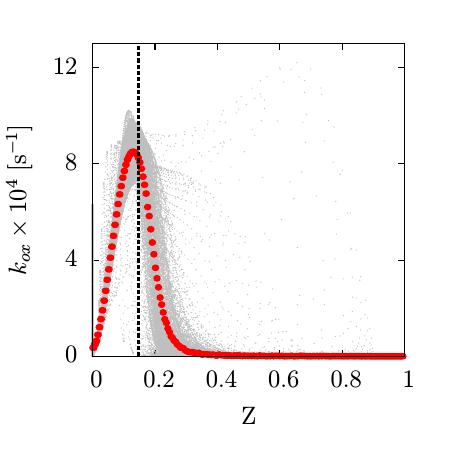
\includegraphics[width=0.43\linewidth]{ch-subfiltermodeling/figures/koxvsz}
  \caption[Approximation for Oxidation Coefficient, $k_{ox}(Z)$]{Density-weighted, conditionally averaged approximation for the oxidation coefficient $k_{ox}(Z)$. The gray dots represent $k_{ox}(x_j)|Z(x_j)$ from DNS and the red circles are the approximation $\{ k_{ox}(x_j)|Z(x_j) \}$, evaluated with 200 bins. The vertical black dashed line marks the location of stoichiometric mixture fraction $Z_{st} = 0.147$.}
  \label{fig:subfilter:dns:kox}
\end{figure}

The second quantity that needs to be estimated is the subfilter PDF for mixture fraction $\pz$, since the DNS database does not have the infinite number of points required to construct the true statistical distribution. As before, this work will presume the form of a beta distribution for $\pz$. The error associated with this assumption can be discerned by juxtaposing two versions of \cref{eq:subfilter:zussp:ox} that use the same $Z$-Uniform Soot Subfilter PDF, but approximate $k_{ox}(Z)$ with and without $\pz$. The form of the filtered moment source term for oxidation that excludes $\pz$ shall be referred to as the ``ZUSSP without $\pz$'' case and is given by
\begin{equation}\label{eq:subfilter:dns:mzusspwithoutpz}
  \fst[M]{1,0}^{ox} = \tf{k}_{ox}(Z(x_j)) \cdot \mean{M_{0,1}(x_j)},
  % \fst[M]{1,0}^{ox} = \{ \tf{k_{ox}(x_j)|Z(x_j)} \} \cdot \mean{M_{0,1}(x_j)}.
\end{equation}
where $k_{ox}(Z(x_j))$ provides the value of the oxidation coefficient at $x_j$ through \cref{eq:subfilter:dns:condkox}. $\tf{k}_{ox}(Z(x_j))$ is the result of Favre filtering the field given by the latter.

%describes the field where the value of the oxidation coefficient at $x_j$ is given by \cref{eq:subfilter:dns:condkox} based on $Z(x_j)$. $\tf{k}_{ox}(Z(x_j))$ is the result of Favre filtering the latter.
%Use of the $Z$-uniform soot subfilter PDF implies that the soot scalars are assumed to be independent of the thermochemical variables. This property is evident in \cref{eq:subfilter:dns:mzusspwithoutpz}, where the two components are distinctly separated.

The source term using $\pz$ will be referred to as the ``ZUSSP with $\pz$'' case, and is given by
\begin{equation}\label{eq:subfilter:dns:mzusspwithpz}
  \fst[M]{1,0}^{ox} = \int\limits_0^1 \{ k_{ox}(x_j)|Z(x_j) \}\tf{P}(Z; \tf{Z}(x_j),\tf{Z_V}(x_j)) dZ \cdot \mean{M_{0,1}(x_j)}.
  % \fst[M]{1,0}^{ox} = \int\limits_0^1 \{ k_{ox}|Z \}\tf{P}(Z; \tf{Z}(x_j),\tf{Z_V}(x_j)) dZ \cdot \mean{M_{0,1}(x_j)},
\end{equation}
%where $\{ k_{ox}|Z \}$ is the density-weighted, conditionally averaged oxidation coefficient as given in \cref{eq:subfilter:dns:condkox}.
\Cref{eq:subfilter:dns:mzusspwithoutpz,eq:subfilter:dns:mzusspwithpz} are first individually compared to the filtered moment source term from DNS, which will be referred to as the ``DNS'' case, and is given by
\begin{equation}\label{eq:subfilter:dns:mdns}
  \fst[M]{1,0}^{ox} = \mean{ k_{ox}(Z(x_j)) \cdot M_{0,1}(x_j)}.
  % \fst[M]{1,0}^{ox} = \mean{\{ k_{ox}(x_j)|Z(x_j)\} \cdot M_{0,1}(x_j)}.
\end{equation}
These comparisons are visible for a normalized filter width of $\Delta/h = 32$ in \cref{fig:subfilter:dns:erroronbetaox}. The top two plots show that \cref{eq:subfilter:dns:mzusspwithoutpz,eq:subfilter:dns:mzusspwithpz} generally overpredict the oxidation rate compared to the value from DNS. However, when they are compared with each other in the bottom left plot, the sample standard deviation $\sigma$ is roughly an order of magnitude smaller. This suggests that the error associated with presuming the form of a beta distribution for $\pz$ is much less than the error associated with using the $Z$-Uniform Soot Subfilter PDF to evaluate the filtered moment source term for oxidation.

The validity of presuming the beta distribution is more easily elucidated in the bottom right plot of \cref{fig:subfilter:dns:erroronbetaox}, where the cumulative distribution function (CDF) is plotted for $\fst[M]{1,0}^{ox}$. It can be observed that the distance between the lines representing \cref{eq:subfilter:dns:mzusspwithoutpz,eq:subfilter:dns:mzusspwithpz} is generally much less than the deviation between the latter and the source term from DNS at a fixed $\fst[M]{1,0}^{ox}$. These trends hold true for larger filter widths as well. % This trend is not valid when the magnitude of the source term is on the order of $10^2$ to $10^3$, where the error of presuming a beta distribution is commensurate with the error from the form of the soot subfilter PDF. Nevertheless, the most important values of the source term are the largest, where the error associated with presuming the form of a beta distribution for $\pz$ is relatively small.

\begin{figure}[ht]
  \centering
  \begin{subfigure}[b]{0.375\linewidth}
    \centering
    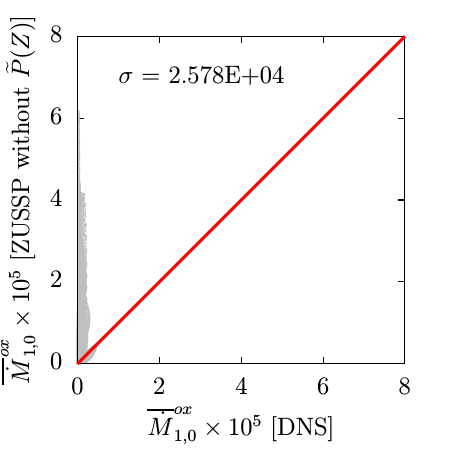
\includegraphics[width=\linewidth]{ch-subfiltermodeling/figures/lin-Mox3vsMox6-r3D-32}
    %\vspace{1ex}
  \end{subfigure}%%
  \begin{subfigure}[b]{0.375\linewidth}
    \centering
    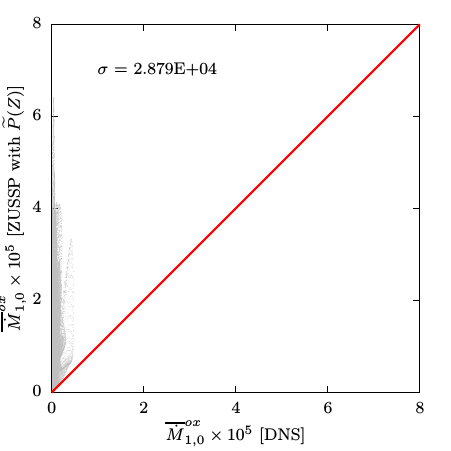
\includegraphics[width=\linewidth]{ch-subfiltermodeling/figures/lin-Mox4vsMox6-r3D-32}
    %\vspace{1ex}
  \end{subfigure}
  \begin{subfigure}[b]{0.375\linewidth}
    \centering
    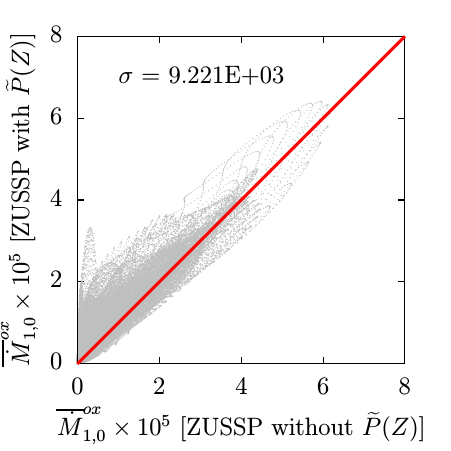
\includegraphics[width=\linewidth]{ch-subfiltermodeling/figures/lin-Mox4vsMox3-r3D-32}
  \end{subfigure}%%
  \begin{subfigure}[b]{0.375\linewidth}
    \centering
    \includegraphics[width=\linewidth]{ch-subfiltermodeling/figures/linear-cdf-ox-ZUSSP-r3D-32}
  \end{subfigure}
  \caption[Error Associated with \texorpdfstring{$\pz = \beta(Z;\tf{Z},\tf{Z_V})$}{P(Z) = B(Z;Z,ZV)} for \texorpdfstring{$\fst[M]{1,0}^{ox}$}{M1,0ox}]{Filtered moment source term for oxidation [m$^3$/(s$\cdot$m$^3$)] at $t = 5$ ms evaluated with \cref{eq:subfilter:dns:mzusspwithoutpz,eq:subfilter:dns:mzusspwithpz,eq:subfilter:dns:mdns} for a normalized filter width of $\Delta/h = 32$. In the first three plots, the red lines represent a one-to-one correspondence and the sample standard deviation is indicated at the top left corner. In the fourth, bottom right plot, the solid red line is the ``DNS'' case, the cyan dashed line is the ``ZUSSP without $\pz$'' case, and the blue dashed line is the ``ZUSSP with $\pz$'' case.}
  \label{fig:subfilter:dns:erroronbetaox}
\end{figure}

Now that the form of $\pz$ has been confirmed, the filtered moment source term for oxidation using the $Z$-Activated Soot Subfilter PDF can be evaluated. The latter shall be referred to as the ``ZASSP with $\pz$'' case, and its expression is given by
\begin{equation}\label{eq:subfilter:dns:mzasspwithpz}
  \fst[M]{1,0}^{ox} = \frac{\int\limits_0^1 \{ k_{ox}(x_j)|Z(x_j) \}H(Z - Z_{st})\tf{P}(Z; \tf{Z}(x_j),\tf{Z_V}(x_j)) dZ}{\int\limits_0^1 H(Z - Z_{st})\tf{P}(Z; \tf{Z}(x_j),\tf{Z_V}(x_j)) dZ} \cdot \mean{M_{0,1}(x_j)}.
  % \fst[M]{1,0}^{ox} = \frac{\int\limits_0^1 \{ k_{ox}|Z \}H(Z - Z_{st})\pz dZ}{\int\limits_0^1 H(Z - Z_{st})\pz dZ} \cdot \mean{M_{0,1}(x_j)}.
\end{equation}

This case is plotted against the source term from DNS in \cref{fig:subfilter:dns:zasspcomparisonox}. In the left-hand plot, it is clear that the source term evaluated with the proposed model still overpredicts the oxidation rate when compared to the values from DNS. However, when contrasted with the top right plot of \cref{fig:subfilter:dns:erroronbetaox}, the magnitudes of the largest source terms are reduced by nearly half. A direct comparison between the source terms using the $Z$-Uniform and $Z$-Activated Soot Subfilter PDFs, available in the middle plot of \cref{fig:subfilter:dns:zasspcomparisonox}, demonstrates that the latter tends to produce smaller oxidation rates than the former. This is expected, for the $Z$-Activated Soot Subfilter PDF was formulated to eliminate the unphysical contributions to the oxidation rate that the $Z$-Uniform Soot Subfilter PDF possessed.

\begin{figure}[ht]
  \centering
  \begin{subfigure}[b]{0.33\linewidth}
    \centering
    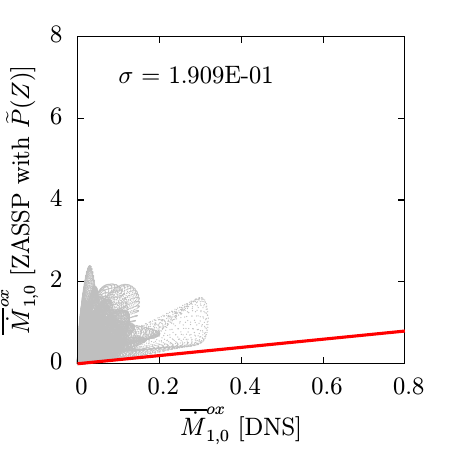
\includegraphics[width=\linewidth]{ch-subfiltermodeling/figures/lin-Mox5vsMox6-r3D-32}
  \end{subfigure}%%
  \begin{subfigure}[b]{0.33\linewidth}
    \centering
    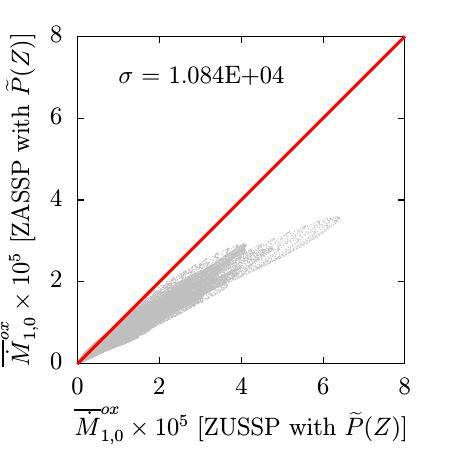
\includegraphics[width=\linewidth]{ch-subfiltermodeling/figures/lin-Mox5vsMox4-r3D-32}
  \end{subfigure}%%
  \begin{subfigure}[b]{0.33\linewidth}
    \centering
    \includegraphics[width=\linewidth]{ch-subfiltermodeling/figures/linear-cdf-ox-ZASSP-r3D-32}
  \end{subfigure}
  \caption[Comparison of ZASSP with \texorpdfstring{$\pz$}{P(Z)} to DNS \& ZUSSP with \texorpdfstring{$\pz$}{P(Z)} for \texorpdfstring{$\fst[M]{1,0}^{ox}$}{M1,0ox}]{Comparison of the ``ZASSP with $\pz$'' case to the ``DNS'' and ``ZUSSP with $\pz$'' cases for the same conditions as in \cref{fig:subfilter:dns:erroronbetaox}. In the right-hand plot, the solid red line is the ``DNS'' case, the blue dashed line is the ``ZUSSP with $\pz$'' case, and the magenta dashed line is the ``ZASSP with $\pz$'' case.}
  \label{fig:subfilter:dns:zasspcomparisonox}
\end{figure}

The CDF in the right-hand plot of \cref{fig:subfilter:dns:zasspcomparisonox} more clearly reveals the extent of the oxidation source term reduction. It is evident that the proposed model has a greater proportion of smaller source terms relative to the ``ZUSSP with $\pz$'' case, albeit the effect is not enough to replicate the CDF from the DNS. Nevertheless, the effectiveness of the proposed model is expected to increase with the filter width due to the expanded presence of lean subfilter regions, which is a consequence of the enlargened variance in mixture fraction. This point will be explored in \cref{sec:subfilter:dns:fw}. Additionally, a model modification that involves rich-shifting the activation location of the sooting mode is expected to further reduce the magnitudes of the oxidation source terms and will be presented in \cref{sec:conclusion:future:zassp}.


\subsection{Surface Growth Source Term}
\label{sec:subfilter:dns:sg}

The $Z$-Activated Soot Subfilter PDF of \cref{sec:subfilter:zassp} has demonstrated the ability to decrease the magnitude of the filtered moment source term for oxidation through the elimination of unphysical contributions at lean mixture fractions. On the other hand, its effect on the source terms for nucleation, condensation, and surface growth has not been investigated yet. These modes of soot evolution are sensitive to the flame structure, and surface growth by the HACA mechanism~\cite{frenklach1985,frenklach1991} can even be a prominent mode of soot growth in near-flame regions, leading to intensified interactions between soot and gas-phase chemistry. However, surface growth is confined to rich regions, so the $Z$-Activated Soot Subfilter PDF is not expected to strongly influence this source term. Confirmation of this hypothesis will be the focus of this subsection.

% Soot oxidation is certainly the dominant mode in these below-stoichiometric regions, but the filtered moment source terms for surface growth could potentially be nonzero, as extrapolation may suggest in \cref{fig:subfilter:leszussp:kvsz}.

% In near-flame regions, surface growth by the HACA mechanism~\cite{frenklach1985,frenklach1991} can be a prominent mode of soot growth and can lead to intensified interactions between soot and gas-phase chemistry. The $Z$-activated soot subfilter PDF was formulated to account for such interactions, so it is worthwhile to analyze its impact on this source term.

As for oxidation, this analysis will investigate the surface growth source term contribution to the total volume fraction, $\fst[M]{1,0}^{sg}$. The aptly named surface growth involves reactions on the soot surface, so the expression for the source term depends on the filtered moment for the total soot surface area $\mean{M}_{0,1}$. As before, the surface growth coefficient $k_{sg}(Z)$ is not present in the DNS database, so it will be taken with a density-weighted conditional average
\begin{equation}\label{eq:subfilter:dns:condksg}
  \begin{split}
    k_{sg}(Z) &\approx \{ k_{sg}(x_j)|Z(x_j) \} \\
    &= \frac{<\rho(x_j)k_{sg}(x_j)|Z(x_j)>}{<\rho(x_j)|Z(x_j)>}.
  \end{split}
\end{equation}
This quantity is plotted in \cref{fig:subfilter:dns:ksg}. The scatter is relatively larger than that of the oxidation coefficient, as expected from \cref{fig:subfilter:leszussp:kvsz}, but, again, modeling of the subfilter PDF is the primary concern here.

%, where it is evident that the surface growth coefficient at mixture fractions $Z < 0.2$ and $Z > 0.4$ is modeled well by \cref{eq:subfilter:dns:condksg}. However, in a similar observation as before, the large spread of the DNS field in $0.2 < Z < 0.4$ indicates that additional conditional averaging against the scalar dissipation rate or another variable could provide a more accurate approximation.

\begin{figure}[htb]
  \centering
  \includegraphics[width=0.43\linewidth]{ch-subfiltermodeling/figures/ksgvsz}
  \caption[Approximation for Surface Growth Coefficient, \texorpdfstring{$k_{sg}(Z)$}{ksg(Z)}]{Density-weighted, conditionally averaged approximation for the surface growth coefficient $k_{sg}(Z)$. All symbols and lines are analogous to those in \cref{fig:subfilter:dns:kox}.}
  \label{fig:subfilter:dns:ksg}
\end{figure}

The subfilter PDF for mixture fraction $\pz$ needs to be modeled as well, and the form of a beta distribution will be presumed. The error associated with this presumption is quantified in \cref{fig:subfilter:dns:erroronbetasg}, where the bottom left plot shows the standard deviation is nearly half of that associated with the form of the soot subfilter PDF (top two plots). The CDF in the bottom right plot reveals that the distance between the lines representing \cref{eq:subfilter:dns:mzusspwithoutpz,eq:subfilter:dns:mzusspwithpz} (adapted for surface growth) is generally less than the distance between the latter and the source term from DNS. Note that the difference between the two errors is not as dramatic as in the CDF from \cref{fig:subfilter:dns:erroronbetaox} for oxidation. Nevertheless, the error associated with presuming the form of a beta distribution for $\pz$ is relatively small for most values of $\fst[M]{1,0}^{sg}$.

% In fact, even at intermediate values of $\fst[M]{1,0}^{sg}$, the error from presuming a beta distribution is comparable to that from the choice of the soot subfilter PDF. Nonetheless, the largest source terms are the most important for this \textit{a priori} analysis as they correspond to heavy growth in the slightly rich, near-flame regions. For these values, the error associated with presuming the form of a beta distribution for $\pz$ is relatively small.

\begin{figure}[ht]
  \centering
  \begin{subfigure}[b]{0.375\linewidth}
    \centering
    \includegraphics[width=\linewidth]{ch-subfiltermodeling/figures/lin-Msg3vsMsg6-r3D-32}
    %\vspace{1ex}
  \end{subfigure}%%
  \begin{subfigure}[b]{0.375\linewidth}
    \centering
    \includegraphics[width=\linewidth]{ch-subfiltermodeling/figures/lin-Msg4vsMsg6-r3D-32}
    %\vspace{1ex}
  \end{subfigure}
  \begin{subfigure}[b]{0.375\linewidth}
    \centering
    \includegraphics[width=\linewidth]{ch-subfiltermodeling/figures/lin-Msg4vsMsg3-r3D-32}
  \end{subfigure}%%
  \begin{subfigure}[b]{0.375\linewidth}
    \centering
    \includegraphics[width=\linewidth]{ch-subfiltermodeling/figures/linear-cdf-sg-ZUSSP-r3D-32}
  \end{subfigure}
  \caption[Error Associated with \texorpdfstring{$\pz = \beta(Z;\tf{Z},\tf{Z_V})$}{P(Z) = B(Z;Z,ZV)} for \texorpdfstring{$\fst[M]{1,0}^{sg}$}{M1,0sg}]{Filtered moment source term for surface growth [m$^3$/(s$\cdot$m$^3$)] at the same conditions of \cref{fig:subfilter:dns:erroronbetaox}. All symbols and lines are analogous to those in \cref{fig:subfilter:dns:erroronbetaox}.}
  \label{fig:subfilter:dns:erroronbetasg}
\end{figure}

The filtered moment source term for surface growth using the $Z$-Activated Soot Subfilter PDF can now be evaluated using an expression analogous to \cref{eq:subfilter:dns:mzasspwithpz}. This case is plotted against the source term from DNS in \cref{fig:subfilter:dns:zasspcomparisonsg}. When the left-hand image is compared to the top right image of \cref{fig:subfilter:dns:erroronbetasg}, the profiles of the source terms utilizing the $Z$-Uniform and $Z$-Activated Soot Subfilter PDFs are nearly identical. This finding indicates that use of the proposed model hardly affects the evaluation of the surface growth source term, which is further confirmed by the middle and right-hand plots of \cref{fig:subfilter:dns:zasspcomparisonsg}. Such a behavior is expected, for the $Z$-Activated Soot Subfilter PDF was formulated to eliminate any unphysical contributions from regions of lean mixture fraction. However, as shown in \cref{fig:subfilter:dns:ksg}, the surface growth coefficient in those regions is negligible. Almost no unphysical contributions exist, so the source term evaluated with the proposed model and the $Z$-Uniform Soot Subfilter PDF should be very similar.
%In the CDF plot of \cref{fig:subfilter:dns:zasspcomparisonsg}, it is also interesting to note that both soot subfilter PDFs tend to overpredict the largest surface growth source terms and underpredict the smallest when compared to the values from DNS.

\begin{figure}[ht]
  \centering
  \begin{subfigure}[b]{0.33\linewidth}
    \centering
    \includegraphics[width=\linewidth]{ch-subfiltermodeling/figures/lin-Msg5vsMsg6-r3D-32}
  \end{subfigure}%%
  \begin{subfigure}[b]{0.33\linewidth}
    \centering
    \includegraphics[width=\linewidth]{ch-subfiltermodeling/figures/lin-Msg5vsMsg4-r3D-32}
  \end{subfigure}%%
  \begin{subfigure}[b]{0.33\linewidth}
    \centering
    \includegraphics[width=\linewidth]{ch-subfiltermodeling/figures/linear-cdf-sg-ZASSP-r3D-32}
  \end{subfigure}
  \caption[Comparison of ZASSP with \texorpdfstring{$\pz$}{P(Z)} to DNS \& ZUSSP with \texorpdfstring{$\pz$}{P(Z)} for \texorpdfstring{$\fst[M]{1,0}^{sg}$}{M1,0sg}]{Comparison of the ``ZASSP with $\pz$'' case to the ``DNS'' and ``ZUSSP with $\pz$'' cases for the same conditions as in \cref{fig:subfilter:dns:erroronbetaox}. All symbols and lines are analogous to those in \cref{fig:subfilter:dns:zasspcomparisonox}.}
  \label{fig:subfilter:dns:zasspcomparisonsg}
\end{figure}


\subsection{Effects of Filter Width}
\label{sec:subfilter:dns:fw}

In grid-filtered LES, the computational expense is directly related to the resolution of the grid. A larger grid spacing reduces the cost but also elevates the cutoff for the length and time scales that need to be modeled. Therefore, it is important to analyze how the proposed model performs as the filter width is increased. As before, the filtered moment source terms for oxidation and surface growth, given by the analogous forms of \cref{eq:subfilter:dns:mzusspwithpz,eq:subfilter:dns:mzasspwithpz}, are the focus of this study. The estimates required for the oxidation and surface growth coefficients have already been investigated in \cref{sec:subfilter:dns:ox,sec:subfilter:dns:sg}, but the error associated with presuming a beta distribution for $\pz$ should be analyzed for an increasing normalized filter width $\Delta/h$. 

\begin{figure}[ht]
  \centering
  \begin{subfigure}[b]{0.33\linewidth}
    \centering
    \includegraphics[width=\linewidth]{ch-subfiltermodeling/figures/linear-cdf-ox-ZUSSP-r3D-4}
  \end{subfigure}%%
  \begin{subfigure}[b]{0.33\linewidth}
    \centering
    \includegraphics[width=\linewidth]{ch-subfiltermodeling/figures/linear-cdf-ox-ZUSSP-r3D-32}
  \end{subfigure}%%
  \begin{subfigure}[b]{0.33\linewidth}
    \centering
    \includegraphics[width=\linewidth]{ch-subfiltermodeling/figures/linear-cdf-ox-ZUSSP-r3D-128}
  \end{subfigure}
  \begin{subfigure}[b]{0.33\linewidth}
    \centering
    \includegraphics[width=\linewidth]{ch-subfiltermodeling/figures/linear-cdf-sg-ZUSSP-r3D-4}
  \end{subfigure}%%
  \begin{subfigure}[b]{0.33\linewidth}
    \centering
    \includegraphics[width=\linewidth]{ch-subfiltermodeling/figures/linear-cdf-sg-ZUSSP-r3D-32}
  \end{subfigure}%%
  \begin{subfigure}[b]{0.33\linewidth}
    \centering
    \includegraphics[width=\linewidth]{ch-subfiltermodeling/figures/linear-cdf-sg-ZUSSP-r3D-128}
  \end{subfigure}
  \caption[Error Associated with \texorpdfstring{$\pz = \beta(Z;\tf{Z},\tf{Z_V})$}{P(Z) = B(Z;Z,ZV)} for Various \texorpdfstring{$\Delta/h$}{D/h}]{CDFs of filtered moment source terms for oxidation (\textit{top}) and surface growth (\textit{bottom}) for normalized filter widths of $\Delta/h = 4$, 32, and 128 (\textit{left to right}). All lines are analogous to those in \cref{fig:subfilter:dns:erroronbetaox}.}
  \label{fig:subfilter:dns:erroronbetafwidth}
\end{figure}

The CDFs of the source terms for oxidation and surface growth are plotted in \cref{fig:subfilter:dns:erroronbetafwidth}. As expected, the ``ZUSSP without $\pz$'' and ``ZUSSP with $\pz$'' cases nearly collapse on the ``DNS'' case for a normalized filter width of 4. The filter width is small enough that presuming a beta distribution for $\pz$ does not have a significant impact on the source term. On the other hand, increasing the normalized filter width to 128 degrades the accuracy of the presumption, especially for the surface growth source term. Presuming a beta distribution may not be appropriate for all conditions, and another distribution may be needed for a more accurate depiction of the subfilter mixture fraction field at large filter widths. Determination of this distribution will be the subject of future work, but, for the remainder of this analysis, the beta distribution will be presumed.

The filtered moment source term for oxidation evaluated with \cref{eq:subfilter:dns:mzasspwithpz} is compared to the source term evaluated with \cref{eq:subfilter:dns:mzusspwithpz} in the top plots of \cref{fig:subfilter:dns:moxfwidth}. For a normalized filter width of 4, the former only slightly underpredicts the rate of oxidation compared to the latter. As the filter width is broadened, the proposed model decreases the oxidation rate more intensely. The CDFs confirm this trend, but the proposed model still overestimates the overall rate of oxidation when compared to the values from DNS.

\begin{figure}[ht]
  \centering
  \begin{subfigure}[b]{0.33\linewidth}
    \centering
    \includegraphics[width=\linewidth]{ch-subfiltermodeling/figures/lin-Mox5vsMox4-r3D-4}
  \end{subfigure}%%
  \begin{subfigure}[b]{0.33\linewidth}
    \centering
    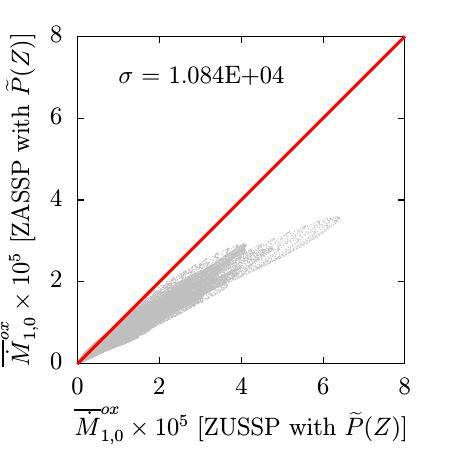
\includegraphics[width=\linewidth]{ch-subfiltermodeling/figures/lin-Mox5vsMox4-r3D-32}
  \end{subfigure}%%
  \begin{subfigure}[b]{0.33\linewidth}
    \centering
    \includegraphics[width=\linewidth]{ch-subfiltermodeling/figures/lin-Mox5vsMox4-r3D-128}
  \end{subfigure}
  %% \begin{subfigure}[b]{0.33\linewidth}
  %%   \centering
  %%   \includegraphics[width=\linewidth]{ch-subfiltermodeling/figures/lin-Mox5vsMox6-r3D-4}
  %% \end{subfigure}%%
  %% \begin{subfigure}[b]{0.33\linewidth}
  %%   \centering
  %%   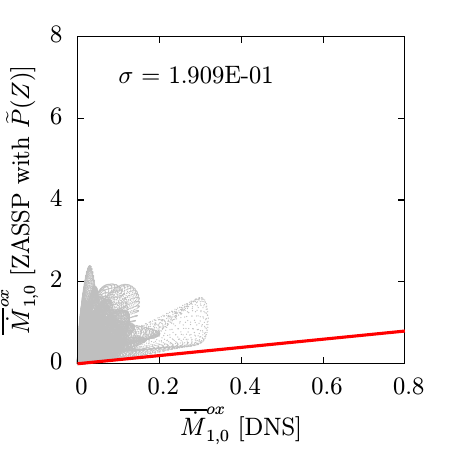
\includegraphics[width=\linewidth]{ch-subfiltermodeling/figures/lin-Mox5vsMox6-r3D-32}
  %% \end{subfigure}%%
  %% \begin{subfigure}[b]{0.33\linewidth}
  %%   \centering
  %%   \includegraphics[width=\linewidth]{ch-subfiltermodeling/figures/lin-Mox5vsMox6-r3D-128}
  %% \end{subfigure}
  \begin{subfigure}[b]{0.33\linewidth}
    \centering
    \includegraphics[width=\linewidth]{ch-subfiltermodeling/figures/linear-cdf-ox-ZASSP-r3D-4}
  \end{subfigure}%%
  \begin{subfigure}[b]{0.33\linewidth}
    \centering
    \includegraphics[width=\linewidth]{ch-subfiltermodeling/figures/linear-cdf-ox-ZASSP-r3D-32}
  \end{subfigure}%%
  \begin{subfigure}[b]{0.33\linewidth}
    \centering
    \includegraphics[width=\linewidth]{ch-subfiltermodeling/figures/linear-cdf-ox-ZASSP-r3D-128}
  \end{subfigure}
  \caption[\texorpdfstring{$\fst[M]{1,0}^{ox}$}{M1,0ox} Using ZASSP with $\pz$ for Various \texorpdfstring{$\Delta/h$}{D/h}]{\textit{Top} - Comparison of the ``ZASSP with $\pz$'' case to the ``ZUSSP with $\pz$'' case at $t = 5$ ms for the oxidation source term. \textit{Bottom} - CDFs of filtered moment source terms for oxidation using the ``ZASSP with $\pz$'' case. Lines for the bottom plots are analogous to those in \cref{fig:subfilter:dns:zasspcomparisonox}. \textit{Left to right} - Normalized filter widths of $\Delta/h = 4$, 32, and 128, respectively.}
  \label{fig:subfilter:dns:moxfwidth}
\end{figure}

The mixture fraction variance increases with the filter width, so the reduction in the oxidation source term can be explained by plotting the ratio of oxidation coefficients from \cref{eq:subfilter:zussp:ox,eq:subfilter:zassp:kox} as a function of the filtered mixture fraction variance. In \cref{fig:subfilter:dns:coeffvszvar}, a growing variance leads to a maximum fivefold reduction in the oxidation coefficient from the proposed model relative to the coefficient from the source term using the $Z$-Uniform Soot Subfilter PDF. %This property is likely the cause for the twofold reduction in the oxidation source term, as shown in the top plots of \cref{fig:subfilter:dns:moxfwidth}.

%% In the CDFs of \cref{fig:subfilter:dns:moxfwidth}, it is also notable that the proportion of source terms with larger values increases with the filter width. The presence of source terms with values greater than $10^3$ becomes dominant at the largest filter width of $\Delta/h = 128$. This suggests that more intense oxidation events occur.

\begin{figure}[htb]
  \centering
  \includegraphics[width=0.43\linewidth]{ch-subfiltermodeling/figures/oxcoeffvszvar-chi10-C7H16}
  \caption[Ratio of Oxidation Coefficients vs. \texorpdfstring{$\tf{Z_{\text{V}}}$}{Zv}]{Ratio of oxidation coefficients versus mixture fraction variance from a flamelet solution for the same nitrogen-diluted, \textit{n}-heptane mixture at $\chi_{st} = 10$ s$^{-1}$. $\tf{k}_{ox}$ is given in \cref{eq:subfilter:zussp:ox}, and $\check{k}_{ox}$ is given in \cref{eq:subfilter:zassp:kox}.}
  \label{fig:subfilter:dns:coeffvszvar}
\end{figure}

The filtered moment source term for surface growth evaluated with the analogous form of \cref{eq:subfilter:dns:mzasspwithpz} is juxtaposed with the analogous source term from \cref{eq:subfilter:dns:mzusspwithpz} in the top plots of \cref{fig:subfilter:dns:msgfwidth}. Although the proposed model overestimates the magnitude of the surface growth rate compared to the source term with the $Z$-Uniform Soot Subfilter PDF, the standard deviations normalized by the maximum source term magnitudes are much less than those of \cref{fig:subfilter:dns:moxfwidth}. Expanding the filter width does not drastically increase the difference between the source terms of \cref{eq:subfilter:dns:mzasspwithpz,eq:subfilter:dns:mzusspwithpz}. This trend agrees with the analysis from \cref{fig:subfilter:dns:zasspcomparisonsg}, where it was found that use of the proposed model hardly affects the evaluation of the surface growth source term. % These observations are especially relevant at the largest values of the surface growth rate even as the filter width is broadened, as shown in the CDF plots of \cref{fig:subfilter:dns:msgfwidth}.

\begin{figure}[ht]
  \centering
  \begin{subfigure}[b]{0.33\linewidth}
    \centering
    \includegraphics[width=\linewidth]{ch-subfiltermodeling/figures/lin-Msg5vsMsg4-r3D-4}
  \end{subfigure}%%
  \begin{subfigure}[b]{0.33\linewidth}
    \centering
    \includegraphics[width=\linewidth]{ch-subfiltermodeling/figures/lin-Msg5vsMsg4-r3D-32}
  \end{subfigure}%%
  \begin{subfigure}[b]{0.33\linewidth}
    \centering
    \includegraphics[width=\linewidth]{ch-subfiltermodeling/figures/lin-Msg5vsMsg4-r3D-128}
  \end{subfigure}
  \begin{subfigure}[b]{0.33\linewidth}
    \centering
    \includegraphics[width=\linewidth]{ch-subfiltermodeling/figures/linear-cdf-sg-ZASSP-r3D-4}
  \end{subfigure}%%
  \begin{subfigure}[b]{0.33\linewidth}
    \centering
    \includegraphics[width=\linewidth]{ch-subfiltermodeling/figures/linear-cdf-sg-ZASSP-r3D-32}
  \end{subfigure}%%
  \begin{subfigure}[b]{0.33\linewidth}
    \centering
    \includegraphics[width=\linewidth]{ch-subfiltermodeling/figures/linear-cdf-sg-ZASSP-r3D-128}
  \end{subfigure}
  \caption[\texorpdfstring{$\fst[M]{1,0}^{sg}$}{M1,0sg} Using ZASSP with $\pz$ for Various \texorpdfstring{$\Delta/h$}{D/h}]{\textit{Top} - Comparison of the ``ZASSP with $\pz$'' case to the ``ZUSSP with $\pz$'' case at $t = 5$ ms for the surface growth source term. \textit{Bottom} - CDFs of filtered moment source terms for surface growth using the ``ZASSP with $\pz$'' case. Lines for the bottom plots are analogous to those in \cref{fig:subfilter:dns:zasspcomparisonox}. \textit{Left to right} - Normalized filter widths of $\Delta/h = 4$, 32, and 128, respectively.}
  \label{fig:subfilter:dns:msgfwidth}
\end{figure}


\chapter{Effect of Transport on PAH Evolution\label{ch:transport}}

The lifetime of soot is governed by the balance between growth and oxidation. Nucleation from collisions between PAH dimers~\cite{blanquart2009,schuetz2002,frenklach1991,wang2011}, condensation of PAH dimers on existing soot particles~\cite{blanquart2009,hmom2009}, and surface growth through the HACA surface reaction mechanism~\cite{frenklach1985,frenklach1991} are processes that increase soot mass by extracting species from the gas-phase. Conversely, oxidation by \ce{OH} and \ce{O2} removes carbon from particles~\cite{stanmore2001,neoh1981,kazakov1995} and can lead to their fragmentation and destruction~\cite{neoh1984,mueller2011}. Clearly, the dynamics of soot are governed by species with a broad range of chemical timescales and molecular weights. Therefore, accurately capturing interactions with gas-phase species is crucial when developing predictive models for soot evolution.

In \cref{ch:lesmodels}, the modeling foundation for LES was established. In particular, the classical nonpremixed flamelet equations for species and temperature~\cite{peters1984} were presented in \cref{sec:lesmodels:combust:flamelet} with modifications accounting for the formation of soot and radiative thermal losses. These equations were derived under the assumption that the species' effective Lewis numbers are unity. This assumption is based on the reasoning that turbulence mixes indiscriminately at sufficiently large Reynolds number~\cite{pitsch19981057}.

%% These equations were derived by transforming the physical space coordinate system of \cref{eq:lesmodels:combust:flamelet:consy,eq:lesmodels:combust:flamelet:const} to a mixture-fraction-based coordinate system. The latter conservation equations used Fick's law to evaluate the diffusion velocity, so all species were assumed to have the same constant diffusion coefficient $D$. A further simplication was made by selecting $D$ such that the species' effective Lewis numbers are unity, for it is often assumed that turbulence mixes all species indiscriminately at sufficiently high Reynolds numbers~\cite{pitsch19981057}.

However, DNS studies~\cite{bisetti2012,attili2014} have suggested that this assumption may be inappropriate for PAH, which are very sensitive to the local scalar dissipation rate due to their slow formation chemistry. These species are confined to spatially intermittent regions of low scalar dissipation rate that are on the order of the Kolmogorov scale or smaller~\cite{vaishnavi2008}. At such scales, transport is solely dictated by molecular diffusion. Therefore, a method to identify such strain-sensitive species and properly account for their interactions with turbulence is desired. The development of a model that addresses these points is the focus of this chapter.

%% Summary: Main point of chapter is to show that existing transport models do not properly account for the presence of soot. As a result, a strain sensitive transport model is developed.

%% Include a brief introduction explaining why accurately capturing the transport of gas-phase species is important for developing predictive models for soot evolution in LES (growth and oxixidation processes).

% include other files for sections of this chapter. These use the 'input' command since each section within a chapter should not start a new page.
% If you want to swap the order of sections, it is as simple as reversing the order you include them. 
\section{Overview of Gas-Phase Species Transport}
\label{sec:transport:overview}

%% \subsection{Equal Effective Diffusivities}
%% \label{sec:transport:overview:le1}

%% Summary of equal effective diffusivities approach.


\subsection{Considerations for PAH}
\label{sec:transport:overview:pah}

The nonpremixed flamelet equations for species and temperature were derived in \cref{sec:lesmodels:combust:flamelet} while assuming that species mass fraction and temperature gradients parallel to the mixture fraction gradient dominate and that the species' effective Lewis numbers are unity. The theory behind the latter assumption states that, at sufficiently large Reynolds number, the smallest scales of turbulence (Kolmogorov scales) penetrate the fuel-oxidizer mixing zone of the nonpremixed flame~\cite{peters1984}. Consequently, turbulent mixing dominates molecular mixing within this region, and all species are transported with unity effective Lewis numbers. This line of reasoning implicitly assumes that the species' length scales are comparable to the fuel-oxidizer mixing length scale, which is certainly true for the major combustion products such as \ce{CO}, \ce{CO2}, \ce{H2}, and \ce{H2O}.

However, the DNS studies of Bisetti \etal~\cite{bisetti2012} and Attili \etal~\cite{attili2014} suggest otherwise for PAH, which play an integral role in soot nucleation and condensation. In \cref{fig:transport:overview:pah:unsteadypah}, the mass fractions of acetylene and naphthalene from the DNS are compared to the values from the one-dimensional steady flamelet equation solutions under the same set of conditions (unity Lewis number, no Soret and Dufour effects, same reduced chemical mechanism, etc.). It is evident that, as the scalar dissipation rate is increased, the mass fraction of acetylene falls from $2 \times 10^{-2}$ to $1 \times 10^{-2}$ while the mass fraction of naphthalene decreases two orders of magnitude from $10^{-4}$ to $10^{-6}$. Naphthalene is clearly more sensitive to the local value of scalar dissipation rate, which is a result of its slow formation chemistry. An elevated local scalar dissipation rate minimizes the time for larger hydrocarbon species to collide and successfully react, so the presence of PAH is restricted to a limited range of low scalar dissipation rates.

\begin{figure}[ht]
  \centering
  \begin{subfigure}[b]{0.375\linewidth}
    \centering
    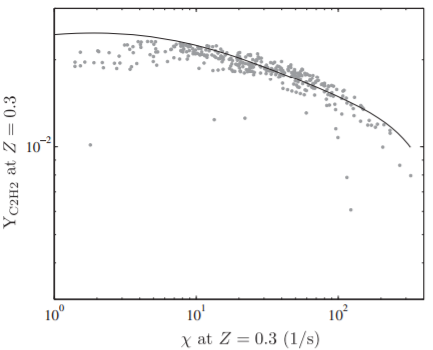
\includegraphics[width=\linewidth]{ch-transport/figures/dns-YC2H2vschi}
  \end{subfigure}%%
  \begin{subfigure}[b]{0.375\linewidth}
    \centering
    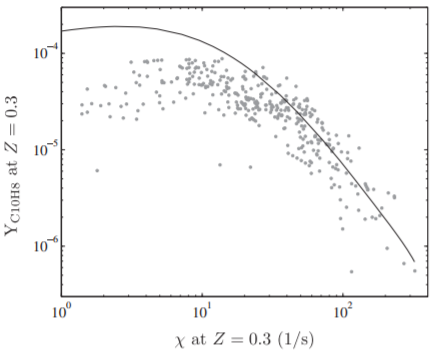
\includegraphics[width=\linewidth]{ch-transport/figures/dns-YC10H8vschi}
  \end{subfigure}
  \caption[Effects of Scalar Dissipation Rate on \texorpdfstring{$Y_{\ce{C2H2}}$}{YC2H2} and \texorpdfstring{$Y_{\ce{C10H8}}$}{YC10H8}]{Mass fraction of acetylene and naphthalene as a function of scalar dissipation rate, reproduced from Bisetti \etal~\cite{bisetti2012}. Samples are taken at $t = 5$ ms and $Z = 0.3$ from the same DNS conditions of \cref{fig:subfilter:zussp:chisensitivity}. Solid lines are the steady flamelet solutions.}
  \label{fig:transport:overview:pah:unsteadypah}
\end{figure} 

Additionally, the steady flamelet solutions tend to capture the overall decreasing trend of the DNS samples for both acetylene and naphthalene, although significant scatter about the steady solution is present for naphthalene. This deviation is caused by naphthalene's inability to adjust to the rapidly changing turbulent flow field and corresponding scalar dissipation rate as a result of its slow chemistry. PAH larger than naphthalene are anticipated to possess similar characteristics. On the other hand, the chemistry of acetylene is much faster, allowing it to persist in regions of larger scalar dissipation rate.
%The scatter is more significant at lower values of scalar dissipation rate, which is due to unsteady flamelet effects~\cite{turbulentcombustion,bisetti2012}.

As a result of the above phenomena, PAH are confined to spatially intermittent regions of low scalar dissipation rate, which are visible in \cref{fig:subfilter:zussp:chisensitivity} for naphthalene. These regions are on the order of the Kolmogorov scale or smaller~\cite{vaishnavi2008}, where transport is solely dictated by molecular diffusion. Therefore, it is worthwhile to examine the effects of molecular transport on the evolution of these soot precursors. Flamelet models that incorporate differential diffusion are presented in the following subsection.


\subsection{Molecular Transport}
\label{sec:transport:overview:lei}

Pitsch and Peters~\cite{pitsch1998} previously derived a set of one-dimensional nonpremixed flamelet equations for flat flames accounting for differential diffusion effects. Assuming variable, nonunity species Lewis numbers and a unity mixture fraction Lewis number, the species equation is given by
\begin{equation}\label{eq:transport:overview:lei:flamelety}
  \rho\pder[Y_k]{\tau} = \frac{\rho\chi}{2 Le_k}\sder[Y_k]{Z} + \dot{m}_k + \frac{\rho\chi}{2 Le_k}\frac{Y_k}{W}\sder[W]{Z} + V_k^{DD},
\end{equation}
where the species Lewis numbers $Le_k = \lambda/c_p\rho D_k$ represent the ratio of thermal to mass diffusivities.
%, $D_k = (1 - Y_k)/\sum\limits_{k \neq l} (X_k/D_{k,l})$ is the mixture-averaged diffusivity for species $k$, and $\chi = 2D_Z(\partial Z/\partial x_j)^2$ is the scalar dissipation rate. The diffusion velocities are expressed by the Curtiss-Hirschfelder approximation~\cite{curtiss1949} with a velocity correction to enforce mass conservation. These remaining molecular transport correction terms are lumped into $V_k^{DD}$ and are outlined in Pitsch and Peters~\cite{pitsch1998}. Similarly, the one-dimensional, adiabatic temperature equation is given by
\begin{equation}\label{eq:transport:overview:lei:flamelett}
  \rho c_p \pder[T]{\tau} = \frac{\rho c_p \chi}{2}\sder[T]{Z} + \frac{\rho\chi}{2}\pder[c_p]{Z}\pder[T]{Z} - \sum\limits_{k} h_k\dot{m}_k + \sum\limits_{k} \frac{\rho\chi}{2 Le_k}\left( \pder[Y_k]{Z} + \frac{Y_k}{W}\pder[W]{Z} \right)(c_p - c_{p,k})\pder[T]{Z},
\end{equation}
where $W$ is the molecular weight of the mixture and pressure variations have been neglected. Note that \cref{eq:transport:overview:lei:flamelety,eq:transport:overview:lei:flamelett} have been derived while assuming that the nonpremixed flame is one-dimensional in physical space \textit{a priori}. This assumption is convenient in the limit of a thin, one-dimensional flat flame, but is not appropriate for thick or curved flames. Recently, Xuan \etal~\cite{xuan2014} re-derived the flamelet equations accounting for differential diffusion while assuming that the nonpremixed flame is one-dimensional in mixture fraction space \textit{a posteriori} in order to capture curvature effects. Although the latter formulation will not be used in the remainder of this work, curvature effects can significantly affect transport in mixture fraction space, and analysis of curvature effects on PAH evolution in turbulent nonpremixed combustion is a suggestion for future work.

Attili \etal~\cite{attili2016} conducted two three-dimensional direct numerical simulations of the same configuration as previously described in \cref{sec:subfilter:dns}, with a modified domain size of $L_x \times L_y \times L_z = 105 \times 94 \times 47$ mm. A mixture-averaged transport approach was employed in one DNS, while the other modeled transport of gas-phase species with unity Lewis numbers. These two simulations were compared to analyze the influence of the diffusion model on the flame structure and soot formation. Their results at $t = 15$ ms, shown in \cref{fig:transport:overview:lei:a2vsz}, indicate that acetylene is unaffected by differential diffusion while naphthalene is strongly affected by the molecular transport model. The locations of the peaks for the latter species are the same for both transport models, but the magnitudes vary by more than a factor of two. These trends are consistent across all times in the DNS and suggest the importance of differential diffusion in predicting the yield of naphthalene and other larger PAH. Attili \etal~\cite{attili2016} noted that the mixture-averaged approach lead to smaller amounts of diffusion (larger Lewis number) of naphthalene than the equal diffusivities approach. As a consequence, the naphthalene structures were found to be smaller and characterized by larger peaks. These ultimately affect the formation of soot due to the non-linearity of the soot source terms with respect to the concentration of PAH species.

\begin{figure}[htb]
  \centering
  \includegraphics[width=0.6\linewidth]{ch-transport/figures/DNSComparison-A2-C2H2}
  \caption[DNS Results with \texorpdfstring{$Le = 1$}{Le = 1} and \texorpdfstring{$Le \neq 1$}{Le != 1}, \texorpdfstring{$\langle Y_{\ce{C2H2}}|Z \rangle$}{<YC2H2|Z>} \& \texorpdfstring{$\langle Y_{\text{A2}}|Z \rangle$}{<YA2|Z>} vs. \texorpdfstring{$Z$}{Z}]{Means of acetylene (\ce{C2H2}) and naphthalene (\ce{A2}) mass fraction conditioned on mixture fraction at $t = 15$ ms, reproduced from Attili \etal~\cite{attili2016}. The filled squares are transport with mixture-averaged diffusion, and the open circles are the $Le = 1$ case. The vertical black dashed line marks the location of stoichiometric mixture fraction $Z_{st} = 0.147$.}
  \label{fig:transport:overview:lei:a2vsz}
\end{figure}

On the other hand, it was also observed that the detailed transport model had a less significant influence on predictions of the temperature and the mass fractions of species that participate in the heat-releasing chemistry. In \cref{fig:transport:overview:lei:tvsz}, there is very little difference between the profiles from the two simulations for the temperature and hydroxyl mass fraction. The discrepancy between the transport models is larger for the hydrogen radical mass fraction profile (not shown), although this may be the result of an only moderate Reynolds number. Flamelet solutions with equal effective diffusivities track the unity Lewis number profiles from the DNS fairly well, unlike the solutions with detailed transport, which deviate from the DNS with the corresponding model.

It is clear that there is a simultaneous presence of transport by molecular diffusion for species that are confined to regions on the order of the Kolmogorov scale or smaller and transport by turbulent eddies for species that participate in faster chemistry. A model for gas-phase species transport that attempts to account for unity and nonunity Lewis numbers is presented in the upcoming subsection.

\begin{figure}[htb]
  \centering
  \includegraphics[width=\linewidth]{ch-transport/figures/DNSComparison-T-OH}
  \caption[DNS Results with \texorpdfstring{$Le = 1$}{Le = 1} and \texorpdfstring{$Le \neq 1$}{Le != 1}, \texorpdfstring{$\langle T|Z \rangle$}{<T|Z>}, and \texorpdfstring{$\langle Y_{\ce{OH}}|Z \rangle$}{<YOH|Z>} vs. \texorpdfstring{$Z$}{Z}]{Means of temperature and hydroxyl mass fraction conditioned on mixture fraction at $t = 15$ ms, reproduced from Attili \etal~\cite{attili2016}. The filled squares are transport with mixture-averaged diffusion, and the open circles are the $Le = 1$ case. One-dimensional nonpremixed flamelet solutions are indicated by the dashed lines (mixture-averaged) and solid lines ($Le = 1$). The vertical black dashed line is the same as in \cref{fig:transport:overview:lei:a2vsz}.}
  \label{fig:transport:overview:lei:tvsz}
\end{figure}


\subsection{Bimodal Transport}
\label{sec:transport:overview:bimodal}

% \Cref{eq:transport:overview:lei:flamelety,eq:transport:overview:lei:flamelett} have been observed to overpredict the amount of differential diffusion in the downstream region of a turbulent jet flame~\cite{pitsch2000}. This behavior has been explained by the decreased Reynolds number in that region, where a diminished scalar dissipation rate permits the smallest scales of turbulence to enter the broadened mixing zone.
The flamelet equations of \cref{sec:lesmodels:combust:flamelet} were derived for very high Reynolds number flows, where it is assumed that only turbulent transport is important. Conversely, \cref{eq:transport:overview:lei:flamelety,eq:transport:overview:lei:flamelett} were derived while assuming that only molecular transport matters, which is applicable to laminar flows. However, for a finite Reynolds number, the truth is in between. Recently, Wang~\cite{wang2016} introduced a Reynolds number dependence into the flamelet framework in order to address this point. To measure the degree of differential molecular diffusion, Wang defined a parameter
\begin{equation}\label{eq:transport:overview:bimodal:theta}
  \theta(r)= \frac{r}{1 + r},
\end{equation}
where $r$ is the ratio of the molecular diffusivity to the turbulent diffusivity and is inversely proportional to the Reynolds number. At the limit of an infinite Reynolds number, the influence of molecular diffusion vanishes as transport by turbulent eddies becomes dominant. In this limit, $r$ and $\theta(r)$ both approach zero. Conversely, when the Reynolds number approaches zero in the laminar limit, the effect of molecular diffusion is maximized, and $r$ tends to infinity. For this situation, $\theta(r)$ approaches unity.

Incorporation into \cref{eq:transport:overview:lei:flamelety,eq:transport:overview:lei:flamelett} is achieved by defining an effective Lewis number for species $k$:
\begin{equation}\label{eq:transport:overview:bimodal:lek}
  \hat{Le}_k = \frac{Le_k}{Le_k + \theta(r) \cdot (1 - Le_k)}.
\end{equation}
The form of this nonlinear dependence on $\theta$ was selected based on the analysis of a turbulent mixing layer~\cite{wang2016}. In the limit of infinite Reynolds number, $\theta = 0$ and $\hat{Le}_k = 1$ to model transport by turbulent diffusion. In the laminar limit, $\theta = 1$ and $\hat{Le}_k = Le_k$ to capture the effects of differential diffusion. %This effective Lewis number is not a physical property anymore, but it allows the aforementioned modes of transport to be modeled by simply replacing all instances of $Le_k$ in \cref{eq:transport:overview:lei:flamelety,eq:transport:overview:lei:flamelett}.

Despite its advancements of the flamelet framework, this model is still inappropriate for sooting flames. Wang's approach implicitly assumes that the length scales of all species are on the order of the thickness of the mixing zone, which varies with respect to the turbulent length scales as a function of Reynolds number. As the Reynolds number varies in a certain region, all species are governed by the mode of transport dictated by \cref{eq:transport:overview:bimodal:theta}. However, from \cref{sec:transport:overview:lei}, it is known that PAH are confined to regions that are on the order of the Kolmogorov scale or smaller due to their slow formation chemistry. At these scales, differential molecular diffusion overwhelms transport by turbulent eddies irrespective of the Reynolds number. Therefore, another model must be formulated to account for these properties of PAH and other species that are governed by slow kinetics. An approach that incorporates the idea of differential differential diffusion is introduced in \cref{sec:transport:ssta}.

\section{Strain-Sensitive Transport Approach}
\label{sec:transport:ssta}

\subsection{Model Development}
\label{sec:transport:ssta:framework}

Using the nonpremixed flamelet framework provided by \cref{eq:transport:overview:lei:flamelety,eq:transport:overview:lei:flamelett}, the proposed model applies molecular transport to particular species rather than to all species within regions of a certain Reynolds number. Selection of these species is through the strain-sensitivity parameter
\begin{equation}\label{eq:transport:ssta:framework:ssp}
  \zeta_k \equiv \frac{\rho\chi}{\dot{m}_k^{+}},
\end{equation}
where $\dot{m}_k^{+}$ is the chemical production rate of species $k$. When $\zeta_k > 1$, the rate of local mixing is greater than the formation chemistry rate (\textit{i.e.}, the chemistry is slow). Species $k$ is then identified as strain-sensitive and is confined to scales on the order of Kolmogorov or smaller, where molecular transport is dominant. Conversely, when $\zeta_k < 1$, the formation chemistry is fast, and the effective diffusivity of species $k$ is governed by the turbulent diffusivity. In this case, the length scales are now comparable to those of fuel-oxidizer mixing (such as for major species).

The strain-sensitivity parameter is shown for a selection of gas-phase species relevant to soot in \cref{fig:transport:ssta:framework:sspc7h16}. It is clear that $\zeta_{\text{A2}} > 1$ for any value of mixture fraction, indicating that differential diffusion for gas-phase naphthalene and larger PAH is important. Conversely, the strain-sensitivity parameters for acetylene, hydroxyl, and hydrogen are less than unity at slightly rich conditions, indicating that turbulent transport is dominant. Such a finding agrees with \cref{fig:transport:overview:lei:a2vsz,fig:transport:overview:lei:tvsz}, where differential diffusion is shown to be relevant for naphthalene but not for the other species. At this stage in model development, the minimum value of $\zeta_k$ is used to determine whether or not the species is strain-sensitive. This value provides the most conservative estimate for the species for which differential diffusion is important.

\begin{figure}[htb]
  \centering
  \includegraphics[width=0.43\linewidth]{ch-transport/figures/ZETAvsZ-C7H16-chi_st20}
  \caption[Strain-Sensitivity Parameter $\zeta_k$ for Various Species Within a \ce{C7H16}/\ce{N2} Mixture]{Strain-sensitivity parameter calculated from nonpremixed flamelet solutions for various species at $\chi_{st} = 20$ s$^{-1}$. The nitrogen-diluted, \textit{n}-heptane fuel mixture is the same as in \cref{fig:subfilter:zussp:chisensitivity}. The red line is for A2, the black line is for \ce{C2H2}, the blue line is for \ce{OH}, and the cyan line is for \ce{H}. The vertical black dashed line indicates the stoichiometric mixture fraction.}
  \label{fig:transport:ssta:framework:sspc7h16}
\end{figure}

A new definition of the effective species Lewis number $\check{Le}_k$ is required that depends on $\zeta_k$:
\begin{equation}\label{eq:transport:ssta:framework:lezetai}
  \check{Le}_k(\zeta_k) = \frac{Le_k}{Le_k + H(\min(\zeta_k) - 1)\cdot (1 - Le_k)},
\end{equation}
where $H(\cdot)$ is the Heaviside function. The flamelet equations for species and temperature become
\begin{equation}\label{eq:transport:ssta:framework:flamelety}
  \rho\pder[Y_k]{\tau} = \frac{\rho\chi}{2 \check{Le}_k(\zeta_k)}\sder[Y_k]{Z} + \dot{m}_k + \frac{\rho\chi}{2 \check{Le}_k(\zeta_k)}\frac{Y_k}{W}\sder[W]{Z} + V_k^{DD} - \dot{\rho}Y_k + (\dot{\rho}Z - \dot{m}_Z)\pder[Y_k]{Z}
\end{equation}
and
\begin{equation}\label{eq:transport:ssta:framework:flamelett}
  \begin{split}
    \rho c_p \pder[T]{\tau} &= \frac{\rho c_p \chi}{2}\sder[T]{Z} + \frac{\rho\chi}{2}\pder[c_p]{Z}\pder[T]{Z} - \sum\limits_{k} h_k\dot{m}_k \\
    &+ \sum\limits_{k} \frac{\rho\chi}{2 \check{Le}_k(\zeta_k)}\left( \pder[Y_k]{Z} + \frac{Y_k}{W}\pder[W]{Z} \right)(c_p - c_{p,k})\pder[T]{Z} + \dot{q}_{\text{RAD}} \\
    &+ \dot{H} + c_p(\dot{\rho}Z - \dot{m}_Z)\pder[T]{Z},
  \end{split}
\end{equation}
respectively. The last two terms of \cref{eq:transport:ssta:framework:flamelety} and the terms on the third line of \cref{eq:transport:ssta:framework:flamelett} are the same as those in \cref{eq:lesmodels:combust:flamelet:flamelety,eq:lesmodels:combust:flamelet:flamelett} to account for the removal of PAH from the gas-phase during nucleation and condensation. This framework for the effective Lewis numbers could also accommodate a Reynolds number dependence~\cite{wang2016}, but such a possibility has not been pursued in this thesis.

% This form is similar to that of Wang~\cite{wang2016}, so a Reynolds number dependence could also be added to the model in future work.


\subsection{\textit{A Priori} Analysis}
\label{sec:transport:ssta:dns}

%These profiles are plotted as a function of the Bilger mixture fraction~\cite{bilger1989} in \cref{fig:transport:ssta:dns:chi}.

%% \begin{figure}[htb]
%%   \centering
%%   \includegraphics[width=0.43\linewidth]{ch-transport/figures/chivsZBilger-C7H16-chi_st20}
%%   \caption[Scalar Dissipation Rate for Various Transport Approaches Within a \ce{C7H16}/\ce{N2} Mixture]{Scalar dissipation rates as a function of the Bilger mixture fraction~\cite{bilger1989}, calculated from nonpremixed flamelet solutions at $\chi_{st} = 20$ s$^{-1}$. The nitrogen-diluted, \textit{n}-heptane fuel mixture is the same as in \cref{fig:subfilter:zussp:chisensitivity}. The solid line is for transport with unity Lewis number, the dash-dotted line is for detailed transport, and the double-dashed line is for strain-sensitive transport. The vertical black dashed line indicates the stoichiometric mixture.}
%%   \label{fig:transport:ssta:dns:chi}
%% \end{figure}

%% The flame temperature and the mass fractions of acetylene and naphthalene are also plotted against the Bilger mixture fraction and are provided in \cref{fig:transport:ssta:dns:tc2h2a2vszbilger} for these transport approaches. In the plot for flame temperature, the profile of the proposed model nearly matches that of the unity Lewis number approach, replicating the trend from \cref{fig:transport:overview:lei:tvsz}. This behavior is expected, for the species that participate in the main heat-releasing chemistry have been modeled with unity Lewis numbers. On the other hand, the peak of the detailed transport approach is lower than those of the latter models. This phenomena is due to the high diffusivity of molecular hydrogen, which ``flattens'' out the temperature profile in mixture fraction space. Note that the detailed transport model is not appropriate in the highly turbulent regions of a nonpremixed jet flame.

%% \begin{figure}[ht]
%%   \centering
%%   \begin{subfigure}[b]{0.33\linewidth}
%%     \includegraphics[width=\linewidth]{ch-transport/figures/TvsZBilger-C7H16-chi_st20}
%%   \end{subfigure}%%
%%   \begin{subfigure}[b]{0.33\linewidth}
%%     \includegraphics[width=\linewidth]{ch-transport/figures/YC2H2vsZBilger-C7H16-chi_st20}
%%   \end{subfigure}%%
%%   \begin{subfigure}[b]{0.33\linewidth}
%%     \includegraphics[width=\linewidth]{ch-transport/figures/YA2vsZBilger-C7H16-chi_st20}
%%   \end{subfigure}
%%   \caption[\texorpdfstring{$T$}{T}, \texorpdfstring{$Y_{\ce{C2H2}}$}{YC2H2}, and \texorpdfstring{$Y_{\text{A2}}$}{YA2} for Various Transport Approaches Within a \ce{C7H16}/\ce{N2} Mixture]{Mass fractions of acetylene and naphthalene and flame temperature as a function of the Bilger mixture fraction~\cite{bilger1989}, calculated from nonpremixed flamelet solutions at $\chi_{st} = 20$ s$^{-1}$. The nitrogen-diluted, \textit{n}-heptane fuel mixture is the same as in \cref{fig:subfilter:zussp:chisensitivity}. All lines are defined in \cref{fig:transport:ssta:dns:chi}.}
%%   \label{fig:transport:ssta:dns:tc2h2a2vszbilger}
%% \end{figure}

Flamelet solutions using the strain-sensitive transport, detailed transport, and unity Lewis number transport models are obtained by evaluating all approaches at the same stoichiometric scalar dissipation rate for the nitrogen-diluted, \textit{n}-heptane mixture from \cref{sec:subfilter:dns}. The flame temperature and the mass fractions of acetylene and naphthalene are provided in \cref{fig:transport:ssta:dns:tc2h2a2vsz} for these transport approaches. In the plot of the flame temperature, the profile of the proposed model nearly matches that of the unity Lewis number approach, replicating the trend from \cref{fig:transport:overview:lei:tvsz}. This behavior is expected, for the species that participate in the main heat-releasing chemistry have been modeled with unity Lewis numbers. On the other hand, the peak of the detailed transport approach is shifted towards larger mixture fractions. This phenomenon is a result of \textit{n}-heptane's large Lewis number, which contributes to a convective velocity towards richer mixture fractions that is encapsulated by $V_k^{DD}$ in \cref{eq:transport:ssta:framework:flamelety}. Note that the detailed transport model is not appropriate in the highly turbulent regions of a nonpremixed jet flame and that this shifting phenomenon contradicts the results from the DNS~\cite{attili2016}.

% On the other hand, the peak of the detailed transport approach is lower than those of the latter models. This phenomena is due to the high diffusivity of molecular hydrogen, which ``flattens'' out the temperature profile in mixture fraction space.
% The rich-shifting of the peak is a result of \textit{n}-heptane's large Lewis number, which contributes to a convective velocity towards richer mixture fractions that is encapsulated by $V_k^{DD}$ in \cref{eq:transport:ssta:framework:flamelety}. Note that the detailed transport model is not appropriate in the highly turbulent regions of a nonpremixed jet flame.

\begin{figure}[ht]
  \centering
  \begin{subfigure}[b]{0.33\linewidth}
    \includegraphics[width=\linewidth]{ch-transport/figures/TvsZ-C7H16-chi_st20}
  \end{subfigure}%%
  \begin{subfigure}[b]{0.33\linewidth}
    \includegraphics[width=\linewidth]{ch-transport/figures/YC2H2vsZ-C7H16-chi_st20}
  \end{subfigure}%%
  \begin{subfigure}[b]{0.33\linewidth}
    \includegraphics[width=\linewidth]{ch-transport/figures/YA2vsZ-C7H16-chi_st20}
  \end{subfigure}
  \caption[\texorpdfstring{$T$}{T}, \texorpdfstring{$Y_{\ce{C2H2}}$}{YC2H2}, and \texorpdfstring{$Y_{\text{A2}}$}{YA2} for Various Transport Approaches Within a \ce{C7H16}/\ce{N2} Mixture]{Flame temperature and mass fractions of acetylene and naphthalene as a function of mixture fraction, calculated from nonpremixed flamelet solutions at $\chi_{st} = 20$ s$^{-1}$. The nitrogen-diluted, \textit{n}-heptane fuel mixture is the same as in \cref{fig:subfilter:zussp:chisensitivity}. The solid line is for transport with unity Lewis number, the dash-dotted line is for detailed transport, and the double-dashed line is for strain-sensitive transport. The vertical black dashed line indicates the stoichiometric mixture fraction.}
  \label{fig:transport:ssta:dns:tc2h2a2vsz}
\end{figure}

% All lines are defined in \cref{fig:transport:ssta:dns:chi}.
The acetylene and naphthalene mass fractions are available in the middle and right-hand plots of \cref{fig:transport:ssta:dns:tc2h2a2vsz}, respectively. Acetylene was identified as having a relatively fast chemical production rate in \cref{fig:transport:ssta:framework:sspc7h16}, so the profile from the proposed model closely follows the flamelet solution with unity Lewis number. Conversely, naphthalene was classified as being strain-sensitive. Note, in particular, that while the naphthalene mass fraction is significantly increased with the proposed model compared to unity Lewis numbers, it is still smaller than with full detailed transport. Overall, the Strain-Sensitive Transport Approach captures the trends that are observed in \cref{fig:transport:overview:lei:a2vsz}. 


\subsection{Strain-Sensitivity Parameter Dependencies}
\label{sec:transport:ssta:dependencies}

The LES in \cref{ch:lesresults} use a fuel mixture that is different from the nitrogen-diluted, \textit{n}-heptane fuel mixture of the DNS. Therefore, it is worthwhile to investigate the extent to which the strain-sensitivity parameter is dependent on the fuel mixture as well as other variables, such as the choice of chemical mechanism and stoichiometric scalar dissipation rate.

%In \cref{fig:transport:ssta:dependencies:fuelchem}, the strain sensitivity parameter has been plotted for the fuel mixtures of \ce{C2H4}/\ce{H2}/\ce{N2} at 40/41/19\% composition by volume~\cite{mahmoud2017}, pure \ce{C2H4}~\cite{shaddix2010,zhang2011}, and \textit{n}-\ce{C7H16}/\ce{N2} at 15/85\% composition by volume~\cite{bisetti2012,attili2014,attili2015}.
In \cref{fig:transport:ssta:dependencies:fuelchem}, the strain sensitivity parameter has been plotted for the fuel mixtures of \ce{C2H4}/\ce{H2}/\ce{N2} at 40/41/19\% composition by volume~\cite{mahmoud2017} and pure \ce{C2H4}~\cite{shaddix2010,zhang2011}. It is obvious that the species identified as strain-sensitive are the same across different fuel mixtures. The minimum value of the parameter for naphthalene is greater than unity for both mixtures, indicating that its transport should be modeled with molecular diffusion. Conversely, the minimum values of acetylene, hydroxyl, and hydrogen are less than unity. These species are not constrained to scales that are on the order of the Kolmogorov scales or smaller, so their transport is governed by turbulent eddies.
%It is obvious that the choice of the fuel mixture does not affect the ability of the strain-sensitivity parameter to identify species with slow production rates.

\begin{figure}[ht]
  \centering
  \begin{subfigure}[b]{0.33\linewidth}
    \includegraphics[width=\linewidth]{ch-transport/figures/ZETAvsZ-EHN-chi_st20}
  \end{subfigure}%%
  \begin{subfigure}[b]{0.33\linewidth}
    \includegraphics[width=\linewidth]{ch-transport/figures/ZETAvsZ-C2H4-chi_st20}
  \end{subfigure}%%
  \begin{subfigure}[b]{0.33\linewidth}
    \includegraphics[width=\linewidth]{ch-transport/figures/ZETAvsZ-C2H4-RedHept-chi_st20}
  \end{subfigure}
  %% \begin{subfigure}[b]{0.33\linewidth}
  %%   \includegraphics[width=\linewidth]{ch-transport/figures/ZETAvsZ-C7H16-chi_st20}
  %% \end{subfigure}
  \caption[Dependencies of Strain-Sensitivity Parameter \texorpdfstring{$\zeta_k$}{Zk} on Fuel Mixture and Chemical Mechanism]{Strain-sensitivity parameter calculated from nonpremixed flamelet solutions for various species at $\chi_{st} = 20$ s$^{-1}$. \textit{Left} - Fuel mixture of \ce{C2H4}/\ce{H2}/\ce{N2} (40/41/19\% by volume)~\cite{mahmoud2017}. \textit{Middle} and \textit{Right} - Fuel is pure \ce{C2H4}~\cite{shaddix2010,zhang2011}. The solutions of the left and middle plots are evaluated with a chemical mechanism that accounts for the formation and oxidation of PAH up to cyclopenta[cd]pyrene (\ce{C18H10})~\cite{blanquart2009588,narayanaswamy2010}, while the profiles in the right plot are from a reduced mechanism that accounts for PAH up to naphthalene (\ce{C10H8})~\cite{bisetti2012}. The lines are the same as in \cref{fig:transport:ssta:framework:sspc7h16}.} %\textit{Right} - Fuel mixture of \textit{n}-\ce{C7H16}/\ce{N2} (15/85\% by volume)~\cite{bisetti2012,attili2014,attili2015}. The solutions of the left and middle plots are evaluated with a chemical mechanism that accounts for the formation and oxidation of PAH up to cyclopenta[cd]pyrene (\ce{C18H10})~\cite{blanquart2009588,narayanaswamy2010}, while the profiles in the right plot are from a reduced mechanism that accounts for PAH up to naphthalene (\ce{C10H8})~\cite{bisetti2012}. The lines are the same as in \cref{fig:transport:ssta:framework:sspc7h16}.}
  \label{fig:transport:ssta:dependencies:fuelchem}
\end{figure}

Additionally, the strain-sensitivity parameter is robust to the choice of chemical mechanism. The left and middle plots of \cref{fig:transport:ssta:dependencies:fuelchem} use a detailed mechanism that contains chemistry for soot precursors with up to eighteen carbon atoms~\cite{blanquart2009588,narayanaswamy2010}, while the plot on the right uses a reduced mechanism that accounts for PAH only up to naphthalene~\cite{bisetti2012}. The same species are identified as strain-sensitive with each chemical mechanism. 

Analysis of the parameter's dependency on the stoichiometric scalar dissipation rate is also fruitful for understanding model performance in various regions of the turbulent flame. The strain-sensitivity parameter is plotted for $\chi_{st} = 0.1$, 1, and 10 s$^{-1}$ in the left, middle, and right plots of \cref{fig:transport:ssta:dependencies:chist}, respectively. It is clear that the same species are identified as strain-sensitive, irrespective of the scalar dissipation rate.

% It is interesting to note that as the stoichiometric scalar dissipation rate decreases, all lines shift downwards. As the rate of turbulent mixing decreases, the chemical production rates of all species become relatively substantial. It can be anticipated that at a low enough stoichiometric scalar dissipation rate, the minimum value of the parameter for naphthalene may become less than unity. In this situation, its rate of formation overtakes the rate of turbulent mixing, so it is no longer constrained to regions on the order of the Kolmogorov scale or smaller. At the same time, the Kolmogorov eddies begin to penetrate the flame's mixing zone, which is broadened at low scalar dissipation rates. Consequently, naphthalene and larger PAH would be transported with unity Lewis numbers under these conditions.

\begin{figure}[ht]
  \centering
  \begin{subfigure}[b]{0.33\linewidth}
    \includegraphics[width=\linewidth]{ch-transport/figures/ZETAvsZ-EHN-chi_st01}
  \end{subfigure}%%
  \begin{subfigure}[b]{0.33\linewidth}
    \includegraphics[width=\linewidth]{ch-transport/figures/ZETAvsZ-EHN-chi_st1}
  \end{subfigure}%%
  \begin{subfigure}[b]{0.33\linewidth}
    \includegraphics[width=\linewidth]{ch-transport/figures/ZETAvsZ-EHN-chi_st10}
  \end{subfigure}
  \caption[Dependency of Strain-Sensitivity Parameter \texorpdfstring{$\zeta_k$}{Zk} on \texorpdfstring{$\chi_{st}$}{Xst}]{Strain-sensitivity parameter calculated from nonpremixed flamelet solutions at various values of stoichiometric scalar dissipation rate. The fuel mixture consists of \ce{C2H4}/\ce{H2}/\ce{N2} (40/41/19\% by volume)~\cite{mahmoud2017}, and the detailed chemical mechanism previously mentioned is used~\cite{blanquart2009588,narayanaswamy2010}. \textit{Left}: $\chi_{st} = 0.1$ s$^{-1}$. \textit{Middle}: $\chi_{st} = 1$ s$^{-1}$. \textit{Right}: $\chi_{st} = 10$ s$^{-1}$. The lines are the same as in \cref{fig:transport:ssta:framework:sspc7h16}.}
  \label{fig:transport:ssta:dependencies:chist}
\end{figure}

% At the other extreme, a high enough rate of turbulent mixing may cause the minimums of all lines to shift above unity. Note, however, that this condition may be unreachable for species like hydrogen and hydroxyl. For instance, the scalar dissipation would have to increase by three orders of magnitude in order for hydroxyl to be considered strain-sensitive. Such a value would certainly be far beyond the stoichiometric scalar dissipation rate at extinction. Additionally, naphthalene would cease to exist at such elevated levels of turbulence.

The corresponding plots for the mass fractions of acetylene and naphthalene evaluated with detailed transport, strain-sensitive transport, and unity Lewis number transport are available in \cref{fig:transport:ssta:dependencies:c2h2a2vschist}. As the stoichiometric scalar dissipation rate is increased from 0.1 s$^{-1}$ to 10 s$^{-1}$, the differences between the various transport models are generally magnified for both species. This is explained by the thinning of the flame structure, which intensifies the effects of molecular diffusion at high scalar dissipation rates. The abatement of gradients in all naphthalene profiles over mixture fraction space further confirms this phenomenon. Additionally, the acetylene mass fraction does not change by more than 20\% for any transport approach as the scalar dissipation rate is increased. Conversely, an increase of two orders of magnitude in the scalar dissipation rate leads to a drop in the mass fraction of naphthalene by roughly an order of magnitude.

\begin{figure}[ht]
  \centering
  \begin{subfigure}[b]{0.33\linewidth}
    \centering
    \includegraphics[width=\linewidth]{ch-transport/figures/YC2H2vsZ-EHN-chi_st01}
  \end{subfigure}%%
  \begin{subfigure}[b]{0.33\linewidth}
    \centering
    \includegraphics[width=\linewidth]{ch-transport/figures/YC2H2vsZ-EHN-chi_st1}
  \end{subfigure}%%
  \begin{subfigure}[b]{0.33\linewidth}
    \centering
    \includegraphics[width=\linewidth]{ch-transport/figures/YC2H2vsZ-EHN-chi_st10}
  \end{subfigure}
  \begin{subfigure}[b]{0.33\linewidth}
    \centering
    \includegraphics[width=\linewidth]{ch-transport/figures/YA2vsZ-EHN-chi_st01}
  \end{subfigure}%%
  \begin{subfigure}[b]{0.33\linewidth}
    \centering
    \includegraphics[width=\linewidth]{ch-transport/figures/YA2vsZ-EHN-chi_st1}
  \end{subfigure}%%
  \begin{subfigure}[b]{0.33\linewidth}
    \centering
    \includegraphics[width=\linewidth]{ch-transport/figures/YA2vsZ-EHN-chi_st10}
  \end{subfigure}
  \begin{subfigure}[b]{0.33\linewidth}
    \centering
    \includegraphics[width=\linewidth]{ch-transport/figures/YOHvsZ-EHN-chi_st01}
  \end{subfigure}%%
  \begin{subfigure}[b]{0.33\linewidth}
    \centering
    \includegraphics[width=\linewidth]{ch-transport/figures/YOHvsZ-EHN-chi_st1}
  \end{subfigure}%%
  \begin{subfigure}[b]{0.33\linewidth}
    \centering
    \includegraphics[width=\linewidth]{ch-transport/figures/YOHvsZ-EHN-chi_st10}
  \end{subfigure}
  \caption[Trends of \texorpdfstring{$Y_{\ce{C2H2}}$}{YC2H2}, \texorpdfstring{$Y_{\text{A2}}$}{YA2}, and \texorpdfstring{$Y_{\ce{OH}}$}{YOH} with \texorpdfstring{$\chi_{st}$}{Xst}]{Mass fractions of acetylene, naphthalene, and hydroxyl as a function of mixture fraction at various values of stoichiometric scalar dissipation rate. \textit{Left}: $\chi_{st} = 0.1$ s$^{-1}$. \textit{Middle}: $\chi_{st} = 1$ s$^{-1}$. \textit{Right}: $\chi_{st} = 10$ s$^{-1}$. The fuel mixture and chemical mechanism are the same as in \cref{fig:transport:ssta:dependencies:chist}. The lines are the same as in \cref{fig:transport:ssta:dns:tc2h2a2vsz}.}
  \label{fig:transport:ssta:dependencies:c2h2a2vschist}
\end{figure}

For acetylene, the flamelet solution with strain-sensitive transport closely follows the profile from the unity Lewis number approach for all values of stoichiometric scalar dissipation rate. This behavior is attributed to acetylene's relatively fast production rate even in the presence of elevated turbulent mixing, as was shown in \cref{fig:transport:ssta:dependencies:chist}. On the other hand, naphthalene is identified as being strain-sensitive, so the proposed model tends to follow the profile from detailed transport. It is interesting to note that at $\chi_{st} = 0.1$ s$^{-1}$ and 1 s$^{-1}$, the proposed model predicts higher levels of naphthalene than the flamelet solution with full detailed transport. This may be the result of the relatively larger amounts of \ce{OH} with detailed transport versus with strain-sensitive transport, as shown in the bottom left and middle plots of \cref{fig:transport:ssta:dependencies:c2h2a2vschist}.

Ultimately, the Strain-Sensitive Transport Approach is an attempt to more accurately model the variety of species that play a role in the evolution of soot. In \cref{fig:transport:ssta:dependencies:c2h2a2vschist}, this proposed model has consistently predicted larger amounts of naphthalene than the unity Lewis number transport approach. The elevated levels of these soot precursors, sometimes by more than a factor of two at certain stoichiometric scalar dissipation rates, could potentially translate into an increase of the soot volume fraction by a factor of four or more over the unity Lewis number approach~\cite{hmom2009}. Results from Large Eddy Simulations with the proposed model as well as with the other transport models are presented in the following chapter.


\chapter{Large Eddy Simulation of Turbulent Nonpremixed Jet Flames\label{ch:lesresults}}

%Summary: This chapter covers all details on the experimental and computational framework used and the LES results that have incorporated the previous models discussed.

The $Z$-activated soot subfilter PDF and the strain-sensitive transport approach have been motivated and developed in \cref{ch:subfilter,ch:transport}. These models are now validated against experimental data from a series of turbulent nonpremixed simple jet flames in this chapter. Before these results are presented, the experimental and computational framework are outlined. 

\section{Experimental Framework}
\label{sec:lesresults:exp}

A series of turbulent nonpremixed ethylene-hydrogen-nitrogen [40/41/19 by volume] jet flames~\cite{mahmoud2017} is used to validate the $Z$-activated soot subfilter PDF of \cref{sec:subfilter:zassp} and the strain-sensitive transport approach of \cref{sec:transport:ssta}. In this series, three attached flames at atmospheric pressure are maintained at a jet exit Reynolds number of 15,000 while the exit strain rate is varied by altering the ratio of the fuel exit velocity to the fuel jet diameter. Surrounding each burner is a contraction with a square cross-section of dimensions 150 mm by 150 mm, from which a uniform coflow of air at a velocity of 1.1 m/s is emitted. Mahmoud \etal~\cite{mahmoud2017} selected ethylene (\ce{C2H4}) for the fuel due to its relatively well-studied chemical kinetics and high soot yield and included hydrogen (\ce{H2}) in the mixture to ensure the attachment of each flame to the burner. Nitrogen (\ce{N2}) was added to the fuel mixture in order to achieve the Reynolds number of 15,000 and reduce the amount of soot produced to enable accurate measurements. \cref{tab:subfilter:leszussp:ehn} summarizes other key aspects of the experimental setup, and complete details can be obtained from Mahmoud \etal~\cite{mahmoud2017}.

\begin{table}[htbp]
\centering
\caption[Flow Conditions of Turbulent Nonpremixed \ce{C2H4}/\ce{H2}/\ce{N2} Jet Flames]{Flow conditions of turbulent nonpremixed \ce{C2H4}/\ce{H2}/\ce{N2} jet flames~\cite{mahmoud2017}}
\label{tab:subfilter:leszussp:ehn}
\begin{tabular}{p{0.35\textwidth} p{0.1\textwidth} p{0.12\textwidth} p{0.12\textwidth} p{0.12\textwidth}}
\toprule
\textbf{Flame} & & \bm{$1/\tau|_{H}$} & \bm{$1/\tau|_{M}$} & \bm{$1/\tau|_{L}$} \\
\midrule

Central jet diameter, $D$
& [mm] & 4.4 & 5.8 & 8.0 \\[0.2em]

Mean jet exit velocity, $U$
& [m/s] & 56.8 & 42.4 & 31.5 \\[0.2em]

Exit strain rate, $U/D$
& [s$^{-1}$] & 12,900 & 7300 & 4300 \\[0.2em]

Exit Reynolds number, $Re_D$
& [--] & 15,000 & 15,000 & 15,000 \\[0.2em]

Mean flame length, $L_f$
& [mm] & 710 & 930 & 1060 \\

\bottomrule
\end{tabular}
\end{table}

In \cref{tab:subfilter:leszussp:ehn}, the flame length, $L_f$, was estimated from five instantaneous photographs of the flames. It is a measure of the distance from the jet exit to the most visible downstream portion of the flame and is repeatable to within 5\% uncertainty~\cite{mahmoud2017}. Measurements of flame temperature and soot volume fraction were taken from thermocouple readings at the centerline and from laser-induced incandescence (LII) signals, respectively. LII was performed with a pulsed Nd:YAG laser at 1064 nm, which emitted a laser sheet with a height of 24 mm that was aligned vertically with the burner axis and transmitted horizontally through the flame. To minimize the effects of fluence variation from attenuation and beam steering, the laser fluence was maintained above 0.5 J/cm$^2$, and statistical data were sampled only from the laser-in half of the flame~\cite{mahmoud2017,sun2015}.

The incandescence was filtered at 430$\pm$10 nm and collected with an intensified CCD camera. The CCD camera's gate-width was set to 50 ns in order to decrease the sensitivity of the signal to the soot particle size~\cite{vanderwal1996,mahmoud2017}. Conversion of the LII signal to the soot volume fraction was accomplished by calibrating against a flat premixed \ce{C2H4}/air flame on a McKenna burner. The volume fraction detection threshold for the collected data is 1 part per billion (ppb), and the uncertainty of the measurements is 25\%.

% Discuss Adelaide flame series details.

\section{Computational Framework}
\label{sec:lesresults:comput}

Grid filtered LES is achieved through NGA, a finite difference code for low-Mach number turbulent reacting flows~\cite{desjardins2008}. The conservation equations for mass and momentum are spatially discretized with second order, central difference operators, and the transport equations for the scalars are spatially discretized with the third order, Weighted Essentially Non-Oscillatory scheme~\cite{jiang1996}. All subfilter stresses and fluxes are closed with the dynamic procedure~\cite{germano1991,lilly1992,moin1991} with Lagrangian averaging over flow path lines~\cite{meneveau1996,reveillon1996}.

The computational domain of each flame consists of a structured grid with $192 \times 96 \times 32$ points in the streamwise, radial, and circumferential directions, respectively. This corresponds to a domain with lengths $200D$ in the streamwise direction and $60D$ in the radial direction, where the grid is stretched for both. The boundary conditions for each domain require an additional simulation of a three-dimensional, fully developed turbulent periodic pipe flow with an average streamwise velocity that matches the corresponding mean jet exit velocity for each case of \cref{tab:subfilter:leszussp:ehn}. The data from these simulations become the inflow conditions within the burner, which is modeled with a single grid point in the streamwise direction. The secondary air coflow is prescribed as a bulk flow of magnitude 1.1 m/s. The downstream exit of the domain is modeled with a convective outflow that globally conserves mass~\cite{akselvoll1996}, and the outer edge of the domain in the radial direction is modeled with a slip wall.

Each computational domain is decomposed with 128 processors. The specific computational cost of each LES is between 2.07 $\mu$s/s and 8.31 $\mu$s/s and varies with the combination of models used. For each LES, statistics were collected over a period in the range 277 ms to 1216 ms, with an average of 605 ms. The total computational cost of each LES ranged from approximately 86,000 cpu-hours to 235,000 cpu-hours for a cumulative total of 1.8 million cpu-hours over all simulations. %The latter and other simulation details are presented in \cref{tab:lesresults:comput:details}. NEED TO FINISH THIS TABLE.

%% \begin{table}[htbp]
%% \centering
%% \caption[LES Computational Details]{LES Computational Details}
%% \label{tab:lesresults:comput:details}
%% \begin{tabular}{p{0.35\textwidth} p{0.1\textwidth} p{0.12\textwidth} p{0.12\textwidth} p{0.12\textwidth}}
%% \toprule
%% \textbf{Flame} & & \bm{$1/\tau|_{H}$} & \bm{$1/\tau|_{M}$} & \bm{$1/\tau|_{L}$} \\
%% \midrule

%% Central jet diameter, $D$
%% & [mm] & 4.4 & 5.8 & 8.0 \\[0.2em]

%% Mean jet exit velocity, $U$
%% & [m/s] & 56.8 & 42.4 & 31.5 \\[0.2em]

%% Exit strain rate, $U/D$
%% & [s$^{-1}$] & 12,900 & 7300 & 4300 \\[0.2em]

%% Exit Reynolds number, $Re_D$
%% & [--] & 15,000 & 15,000 & 15,000 \\[0.2em]

%% Mean flame length, $L_f$
%% & [mm] & 710 & 930 & 1060 \\

%% \bottomrule
%% \end{tabular}
%% \end{table}


\subsection{Radiation Model}
\label{sec:lesresults:comput:rad}

In \cref{sec:lesmodels:combust}, the RFPV approach~\cite{ihme2008} was selected for the turbulent combustion model to account for radiative losses. Radiation is modeled with a gray gas approach, where the absorption coefficients for \ce{CO2}, \ce{H2O}, \ce{CH4}, and \ce{CO} are obtained from Barlow \etal~\cite{barlow2001}. Since soot radiation is included in addition to gas-phase radiation, the corresponding absorption coefficients are taken from Hubbard and Tien~\cite{hubbard1978}.


\subsection{Chemical Mechanisms}
\label{sec:lesresults:comput:chem}

The databases of solutions to the steady flamelet equations with radiative losses are computed with FlameMaster, a solver for 0D combustion and 1D laminar flame calculations~\cite{flamemaster}. Seven databases were generated to account for different combinations of chemical mechanisms, soot subfilter PDFs, and subfilter transport models. Five of the databases utilize the chemical mechanism of Blanquart \etal~\cite{blanquart2009588}, which encompasses the high temperature combustion of fuels from methane to iso-octane and places emphasis on the formation of soot precursors up to cyclopenta[cd]pyrene (\ce{C18H10}). The mechanism of Narayanaswamy \etal~\cite{narayanaswamy2010} is incorporated into the base mechanism to model the high-temperature oxidation of aromatic species. In total, there are 158 species and 1804 reactions. The remaining two databases use the chemical mechanism of Wang \etal~\cite{wang2013}, which contains the high temperature kinetics of \ce{C1-C4} hydrocarbons fuels and accounts for the formation and growth of PAH up to coronene (\ce{C24H12}). This mechanism, referred to as KM2, includes 202 species and 1351 reactions.

These databases are parameterized by $\tf{Z}$, $\tf{Z_V}$, $\tf{C}$, and $\tf{H}$, as previously discussed in \cref{sec:lesmodels:presumedpdf}, and have a resolution of 100 divisions for each parameter. Additionally, each database accounts for soot variables in addition to the quantities required for the RFPV approach~\cite{ihme2008}, so the LES code has been parallelized using a hybrid method of one MPI process per cluster node and sixteen OpenMP threads per node to accommodate the large memory requirement of each database.

\section{Flow Field Boundary Conditions}
\label{sec:lesresults:bc}

As discussed in \cref{sec:lesresults:comput}, additional LES of three-dimensional, fully developed turbulent periodic pipe flows are required to generate the flow field conditions within each burner. These flow field conditions specify the fuel-side inflow boundary condition of each turbulent nonpremixed jet, so the quality of their enforcement must be assessed through comparison against the experimental data. 

Radial profiles of the streamwise velocity component and its root-mean-square counterpart are shown in \cref{fig:lesresults:bc:uurms}. Each profile is normalized by the mean jet exit velocity of flame $1/\tau|_H$. In general, the agreement between LES and the experiments is good. The normalized streamwise velocity component of jet flames $1/\tau|_M$ and $1/\tau|_L$ from LES closely replicates the experimental data within the burner, away from the wall, and in the coflow. However, the velocity is underpredicted around the near-wall region at $r/D = 0.5$, suggesting that there is less mixing between the fuel stream and air coflow in the simulations. On the other hand, the agreement between LES and the experiments is good in the near-wall region and in the coflow of the flame with the largest exit strain rate ($1/\tau|_H$), but is worse in the region near the centerline. The profile from LES underpredicts the experimental values for $r/D < 0.34$, and is ``flatter'' than the measured profile. The latter observation suggests that the turbulent flow inside the burner may not be fully developed in the experiment.
% This reduced amount of mixing may be a result of the grid resolution at the wall, so additional studies are needed to evaluate the impact of refining the grid near the wall. 

The bottom plots of \cref{fig:lesresults:bc:uurms} contain the normalized Root-Mean-Square (RMS) streamwise velocity profiles as a function of the normalized radius. It can be observed that LES follows the general trends of the experiments, where the normalized RMS velocities are zero at large $r/D$ and reach their maximum values just before $r/D = 0.5$, at which point they steadily decline as $r/D$ approaches zero. However, LES generally underpredicts the normalized RMS velocities near $r/D = 0.25$ and overpredicts the maximum values, the extent of which increases with the exit strain rate. These deviations are expected to diminish as the grid resolution is refined, especially in the near-wall region. Ultimately, the discrepancies in the fuel-side flow field boundary condition do not affect the downstream results significantly.

\begin{figure}[htb]
  \centering
  \includegraphics[width=\linewidth]{ch-lesresults/figures/U-URMS}
  \caption[Fuel-Side Flow Field Boundary Conditions]{\textit{Top} - Radial profiles of the normalized streamwise velocity component. \textit{Bottom} - Radial profiles of the normalized streamwise root-mean-square velocity component. \textit{Left to right} - Jet flames $1/\tau|_H$, $1/\tau|_M$, and $1/\tau|_L$, respectively. Circles indicate the experimental data of Mahmoud \etal~\cite{mahmoud2017}, while solid lines are time-averaged values from LES. All data are taken from 2 mm above the burner.}
  \label{fig:lesresults:bc:uurms}
\end{figure}

\section{Z-Activated Soot Subfilter PDF}
\label{sec:lesresults:zassp}

In this section, results from LES with the $Z$-activated soot subfilter PDF of \cref{sec:subfilter:zassp} are compared against experimental data and the results from LES with the $Z$-uniform soot subfilter PDF of \cref{sec:subfilter:zussp}. The focus of this section is to evaluate the differences between the two soot subfilter PDFs, so the effective Lewis numbers of all gas-phase species will be held constant at unity in both LES cases.
% ability of the $Z$-activated soot subfilter PDF to more accurately predict the evolution of soot, so the effective Lewis numbers of all gas-phase species will be held constant at unity in both LES cases.  

In \cref{fig:lesresults:zassp:ctrlineleseval}, it is clear that time-averaged, centerline flame temperature is generally well-predicted by both LES cases in all flames. In the recorded experiments, the flame temperature rises to a peak value around $x/D = 100$. The flame with the highest exit strain rate ($1/\tau|_H$, left plot) possesses a small region of uniform temperature around $x/D = 0$ due to the lifting of the flame in both LES cases. This feature is not present in the experiments and explains the slight downstream shift of the temperature compared to the experiment until about $x/D = 50$. In all three flames, the peak mean temperature from LES closely matches the magnitude of the corresponding experimental value (1800 to 1900 K), but is shifted slightly downstream. Overall, the simulated flames tend to be longer than their experimental counterparts.

\begin{figure}[htb]
  \centering
  \includegraphics[width=\linewidth]{ch-lesresults/figures/combined-Tfv-S-ZUSSP-vs-ZASSP-Le_1}
  \caption[Centerline \texorpdfstring{$\langle T \rangle$}{<T>} \& \texorpdfstring{$\langle f_V \rangle$}{<fV>} from LES with \texorpdfstring{$Z$}{Z}-Activated Soot Subfilter PDF]{\textit{Left to right} - Time-averaged flame temperatures and soot volume fractions from LES of jet flames $1/\tau|_H$, $1/\tau|_M$, and $1/\tau|_L$, respectively. Note that the soot volume fraction profiles from LES have been premultiplied by a factor of 100 for visibility. Circles indicate experimental data, solid lines are time-averaged values from LES with the $Z$-uniform soot subfilter PDF, and dashed lines are time-averaged values from LES with the $Z$-activated soot subfilter PDF. Profiles in black correspond to centerline flame temperatures while profiles in blue represent centerline soot volume fractions.}
  \label{fig:lesresults:zassp:ctrlineleseval}
\end{figure}

Most obvious in \cref{fig:lesresults:zassp:ctrlineleseval} is the underprediction of the time-averaged, centerline soot volume fraction by both LES cases. In all three flames, the volume fraction is underestimated by roughly two orders of magnitude relative to the experimental values. Furthermore, the mean soot volume fractions from each LES peak slightly earlier and approach zero sooner at approximately $x/D = 130$. These phenomena signal the presence of intense oxidation further upstream compared to the experiments. However, the LES with the $Z$-activated soot subfilter PDF do not experience as much oxidation as the LES with the $Z$-uniform soot subfilter PDF, which is evident by the elevated amount of soot volume fraction in the downstream regions of flames $1/\tau|_H$ and $1/\tau|_L$. In jet flame $1/\tau|_M$, the maximum volume fraction of the LES with the $Z$-uniform soot subfilter PDF is slightly larger than that from the LES with the proposed model, which is a result of the less-converged statistics of the former. Overall, the decreased rate of oxidation is expected, as turbulent mixing promotes the presence of regions with mixture fractions less than stoichiometric. The $Z$-activated soot subfilter PDF was formulated to eliminate the unphysical oxidation contributions from these fuel-lean areas, so soot is able to persist slightly further downstream than in the simulations with the $Z$-uniform soot subfilter PDF.

Ultimately, the differences in the predicted centerline volume fractions from the two soot subfilter PDFs are not dramatic. In \cref{fig:subfilter:leszussp:kvsz}, it is evident that implementing a cutoff at the stoichiometric mixture fraction does not appreciably decrease the maximum rate of oxidation. In fact, the rate of oxidation at the latter location is only slightly less than the global maximum of the oxidation rate. To address this point, modifications to the activation location of the $Z$-activated soot subfilter PDF in mixture fraction space are proposed in \cref{sec:conclusion:future:zassp}.

Time-averaged radial statistics of the soot volume fraction source terms are provided in \cref{fig:lesresults:zassp:radialdfvdt}. In jet flames $1/\tau|_M$ and $1/\tau|_L$, the maximum rates of oxidation from LES with the $Z$-activated soot subfilter PDF become smaller than those from LES with the $Z$-uniform soot subfilter PDF as the distance in the streamwise direction is increased. However, as previously mentioned, these differences are minimal. %This trend is especially observable in jet flames $1/\tau|_M$ and $1/\tau|_L$, where the maximum rates of oxidation from LES with the proposed model are initially larger than those from LES with the $Z$-uniform soot subfilter PDF at $x/D = 49$ and 71.

\begin{figure}[H]
  \centering
  \includegraphics[width=\linewidth]{ch-lesresults/figures/dfvdt-S-ZUSSP-vs-ZASSP-Le_1-edited}
  \caption[Radial \texorpdfstring{$\langle df_V/dt \rangle$}{<dfV/dt>} from LES with \texorpdfstring{$Z$}{Z}-Activated Soot Subfilter PDF]{\textit{Left to right} - Time-averaged soot volume fraction source terms from LES of jet flames $1/\tau|_H$, $1/\tau|_M$, and $1/\tau|_L$, respectively. \textit{Bottom to top} - Increasing streamwise locations of $x/D = 49, 71, 94,$ and 117, respectively. Solid lines are LES with the $Z$-uniform soot subfilter PDF and dashed lines are LES with the $Z$-activated soot subfilter PDF. Profiles in green are source terms from nucleation and condensation, profiles in red are source terms from surface growth, and profiles in blue are source terms from oxidation. The soot volume fraction is provided as a reference in the background from $0 \le r/D \le 2$ of each flame, where the positions $x/D = 49, 71, 94,$ and 117 in the field are aligned at the corresponding middle of each plot.}
  \label{fig:lesresults:zassp:radialdfvdt}
\end{figure}

Both subfilter PDFs accurately capture the overall nature of soot evolution with respect to the streamwise distance. The position $x/D = 49$ is approximately located at the beginning of the region of concentrated volume fraction, as revealed by the background field in \cref{fig:lesresults:zassp:radialdfvdt}. Here, nucleation from PAH (and condensation to a lesser degree) are the main soot growth pathways. Condensation becomes increasingly important at $x/D = 71$ (investigation not shown), where nucleated particles are numerous enough for PAH to condense upon. At $x/D = 94$, surface growth overtakes nucleation and condensation as the main growth pathway for jet flames $1/\tau|_H$ and $1/\tau|_M$. Such a transition between the growth modes is reasonable, for turbulent mixing tends to decrease the mixture fraction in the downstream region and promote surface growth, as shown in \cref{fig:subfilter:leszussp:kvsz}. Additionally, the elevated global strain rates in the aforementioned flames tend to decrease the influence of the strain-sensitive PAH. %These observations suggest that the conclusions of previous DNS studies of nonpremixed turbulent flames~\cite{bisetti2012,attili2014} are premature, where these analyses found that the soot mass growth rate from surface reactions is dominated by the contributions from nucleation and condensation processes.

The differences in the surface growth source terms between the LES with the $Z$-activated soot subfilter PDF and the LES with the $Z$-uniform soot subfilter PDF are observed to be minimal at $x/D = 94$. This finding agrees with the \textit{a priori} analysis of \cref{sec:subfilter:dns:sg}, where a comparison of the two soot subfilter PDFs revealed small differences in the evaluation of the surface growth moment source term. Lastly, oxidation dominates all growth modes at $x/D = 117$. %, where the LES with the proposed subfilter PDF predict relatively smaller maximum volume fraction source terms for oxidation.

%% The soot volume fraction is a measure of the total volume of soot relative to the total volume of gas. The amount of soot that is present depends on the rates of nucleation, condensation, surface growth, and oxidation. An underprediction of the volume fraction suggests that soot growth through nucleation, condensation, and surface growth is insufficient, or that soot oxidation is overwhelmingly excessive. Expressions for the filtered moment source terms of these modes are similar in form to \cref{eq:lesmodels:presumedpdf:separated}. For example, the filtered moment source term for oxidation is given by
%% \begin{equation}\label{eq:subfilter:leszussp:ox}
%%   \begin{split}
%%     \mean{\dot{M}}_{x,y}^{ox} &= \iint k_{ox}(Z)\mc{M}_j P(\mc{M}_j)\pz dZ d\mc{M}_j \\
%%     &= \hat{k}_{ox}\mean{M}_j,
%%   \end{split}
%% \end{equation}
%% where $k_{ox}(Z)$ is the oxidation coefficient, $\pz$ is modeled with a beta distribution as in \cref{eq:lesmodels:presumedpdf:trimarg}, and the soot subfilter PDF $P(\mc{M}_j)$ is provided in \cref{eq:subfilter:zussp:dd}. Contributions from the thermochemical and soot variables are made distinct in the second line, where $\hat{k}_{ox} = \int k_{ox}(Z)\pz dZ$ and $\mean{M}_j = \int \mc{M}_j P(\mc{M}_j)d\mc{M}_j$. \cref{eq:subfilter:leszussp:ox} incorporates the joint PDF simplification of Mueller and Pitsch~\cite{subfilterpdf2011}, which postulates that the soot scalars should be independent of the thermochemical variables due to the long timescales of PAH and soot formation relative to the timescales of the highly exothermic combustion chemistry. However, they also noted that such an assumption could be violated when surface growth near the flame is the dominant growth mechanism or during the oxidation of soot, when interactions with gas-phase chemistry are enhanced. The likelihood of the former is smaller, as the DNS studies of Bisetti \etal~\cite{bisetti2012} demonstrated that soot growth through PAH-based nucleation and condensation dominates acetylene-based surface growth in turbulent nonpremixed combustion. Therefore, this work hypothesizes that the excessive oxidation of soot, due to the simplification of the joint subfilter PDF (\cref{eq:lesmodels:presumedpdf:bayes}), is the reason for the dramatic underprediction of the soot volume fraction as shown in \cref{fig:subfilter:leszussp:zusspleseval}.

%% As a result of the decorrelation of the soot scalars from the thermochemical variables, the current soot subfilter PDF implictly assumes that soot is uniformly distributed in mixture fraction space. However, for non-smoking flames, this is qualitatively incorrect as there should be zero soot in fuel-lean regions of the flame. This is evident in \cref{fig:subfilter:leszussp:ysvsz}, reproduced from the 3D DNS of a nitrogen-diluted, \textit{n}-heptane/air turbulent nonpremixed planar jet flame~\cite{attili2014}. The lack of soot at mixture fractions below stoichiometric can be explained by the preferential transport of soot generated in the region $0.3 < Z < 0.5$ to richer mixture fractions by turbulent fluctuations and by the oxidation of all soot during transport towards the stoichiometric surface. 

%% %% \begin{figure}[htb]
%% %%   \centering
%% %%   \includegraphics[width=0.7\linewidth]{ch-subfiltermodeling/figures/dns_Ysoot_vs_Z}
%% %%   \caption[DNS of Turbulent Nonpremixed \ce{C7H16}/\ce{N2} Jet Flame, \texorpdfstring{$\langle Y_{\text{s}}|Z \rangle$}{<Ys|Z>} vs. \texorpdfstring{$Z$}{Z}]{Mean soot mass fraction conditioned on mixture fraction at various times in a 3D DNS of an \textit{n}-heptane/nitrogen [15/85 by volume] and air turbulent nonpremixed planar jet flame, reproduced from Attili \etal~\cite{attili2014}. The stoichiometric mixture fraction ($Z_{st} = 0.147$) is demarcated with the vertical dashed line. \textit{Left} - 1 ms (filled squares), 2 ms (crosses), 3 ms (open squares), 4 ms (circles), and 5 ms (triangles). \textit{Right} - 6 ms (stars), 8 ms (circles), 10 ms (open squares), and 20 ms (filled squares). The small gray dots represent the soot mass fraction field at 20 ms.}
%% %%   \label{fig:subfilter:leszussp:ysvsz}
%% %% \end{figure}

%% The non-uniform nature of soot in mixture fraction space is captured by the flamelet solutions that are accessed during LES as well. Filtered moment source term coefficients for oxidation, surface growth, and the combination of nucleation and condensation are plotted in \cref{fig:subfilter:leszussp:kvsz}. It is clear that different soot evolution modes are dominant over distinct regions of mixture fraction even as the fuel mixture and stoichiometric scalar dissipation rate are varied. Soot growth through PAH-based nucleation and condensation prevails at very rich values of mixture fraction, whereas acetylene-based surface growth is more dominant at moderately rich mixture fractions. It is notable that for a fixed fuel mixture (middle and right plots), a reduction in the value of stoichiometric scalar dissipation rate induces a large increase in the coefficient for nucleation and condensation while the coefficient for surface growth is lessened. This trend is due to the increasing effectiveness of PAH chemistry at smaller values of scalar dissipation rate. Therefore, PAH-based soot growth is supported at leaner conditions, which ultimately supplants acetylene-based surface growth.

%% %% \begin{figure}[htb]
%% %%   \centering
%% %%   \includegraphics[width=\linewidth]{ch-subfiltermodeling/figures/flamelet_sootcoeffs_le1}
%% %%   \caption[Soot Growth and Oxidation Coefficients, 1/\texorpdfstring{$\tau$}{t} vs. \texorpdfstring{$Z$}{Z}]{Flamelet calculations of soot growth and oxidation coefficients for filtered moment source terms as a function of mixture fraction. The blue lines are the oxidation coefficients, the red lines represent the surface growth coefficients, and the green lines are the coefficients for nucleation and condensation. \textit{Left} - Fuel mixture \textit{n}-heptane/nitrogen [15/85 by volume] used in the DNS of \cref{fig:subfilter:zussp:chisensitivity,fig:subfilter:leszussp:ysvsz} at $\chi_{st} = 10\ s^{-1}$. \textit{Middle} \& \textit{Right} - Fuel mixture \ce{C2H4}/\ce{H2}/\ce{N2} [40/41/19 by volume] used in the LES of \cref{fig:subfilter:leszussp:zusspleseval} at $\chi_{st} = 10\ s^{-1}$ and $\chi_{st} = 0.1\ s^{-1}$, respectively.}
%% %%   \label{fig:subfilter:leszussp:kvsz}
%% %% \end{figure}

%% Soot oxidation is the dominant mode at mixture fractions below and slightly above the stoichiometric value. Since the rates associated with the high-temperature oxidation chemistry are comparable with those of the main heat-releasing chemistry~\cite{guo2016}, it is anticipated that the magnitude of the peak oxidation coefficient will not vary much as the fuel mixture or stoichiometric scalar dissipation rate is modified. Indeed, this phenomenon is evident in \cref{fig:subfilter:leszussp:kvsz}. Additionally, the oxidation coefficient at stoichiometric mixture fraction is at least an order of magnitude larger than the maximum value of the surface growth coefficient. Thus, the complete oxidation of soot by \ce{OH} (and \ce{O2} to a lesser degree) is expected during transport towards stoichiometric regions. However, the soot subfilter PDF given by \cref{eq:subfilter:zussp:dd} permits the existence of soot in fuel-lean areas, for it assumes that soot is uniformly distributed in mixture fraction space. Therefore, the presence of large, non-zero oxidation coefficients at lean values of mixture fraction is concerning, for it potentially leads to substantial filtered moment source terms (\cref{eq:subfilter:leszussp:ox}). This contribution to the oxidation rate is artificial and could be an explanation for the underpredicted soot volume fraction in \cref{fig:subfilter:leszussp:zusspleseval}. To prevent this non-physical oxidation from occurring, the subfilter PDF must depend on the thermochemical variables to exclude the presence of soot at lean mixtures $Z < Z_{st}$. A soot subfilter PDF that addresses this point is introduced in the following section.

%% Perhaps have a comparison of flamelets first to give hints at what to expect in terms of $Y_{PAH}$ and $f_V$. Include comparison of EHN, Stanford, $\check{Le}_i(\zeta_i)$, and ZUSSP vs. ZASSP.

%% Talk about temperature, $Y_{PAH}$, $f_V$, conditional radial statistics at various distances downstream, etc.

\section{Strain-Sensitive Transport Approach}
\label{sec:lesresults:ssta}

%% what i want to say in this section: start with a comparison of unity to zeta to lei for flame 2. discuss centerline T and fv.
%% Then bring in radial statistics for unity vs zeta vs lek.

%% next, discuss zeta vs unity across all three flames for centerline T and fv structure.
%% bring in radial statistics for zeta vs unity and discuss T and fv.
%% Then look at radial conditional statistics at xD = 49, 71, 94, and 117 for dfv/dt for nucleation + condensation, surface growth, and oxidation to compare zeta and lek?
%% lastly, bring up point of different chemical mechanism - km2.
%% Show centerline T and fv for KM2 with le1 and le zeta, compare with existing models for flame 2.
%% finally, compare radial statistics for KM2 flame 2 against stanford mechanisms.

Results from the LES using the $Z$-activated soot subfilter PDF were presented in \cref{sec:lesresults:zassp} under the assumption of unity effective Lewis numbers for all gas-phase species. This assumption is appropriate when turbulent transport dominates molecular diffusion within the fuel-oxidizer mixing zone, and when the species' length scales are comparable to the length scale of the latter. In \cref{ch:transport}, this was found to be inappropriate for PAH, whose formation chemistry is slow relative to turbulent mixing. PAH are confined to regions of low scalar dissipation rate that are on the order of the Kolmogorov scale or smaller~\cite{vaishnavi2008}, so they are governed by molecular transport. The strain-sensitive transport approach was developed in \cref{sec:transport:ssta} to more accurately model the behavior of PAH and similar species with relatively slow chemistry. In this section, LES results with the aforementioned approach will be compared to experimental data and LES with other transport models. The goal is to evaluate the ability of the proposed transport model to more accurately predict the evolution of soot, so the $Z$-activated soot subfilter PDF will be implemented in all cases of interest.

In \cref{fig:lesresults:ssta:f2lecomparison}, the time-averaged, centerline flame temperature is plotted for flame $1/\tau|_M$ of \cref{tab:subfilter:leszussp:ehn}. It is clear that the LES with unity effective Lewis numbers and the strain-sensitive transport approach predict the flame temperature fairly accurately, while the LES with detailed transport for gas-phase species predicts a much longer flame with a higher maximum temperature. The peak mean temperatures of the former two LES closely match the magnitude of the experimental value, but are shifted slightly downstream as in \cref{fig:lesresults:zassp:ctrlineleseval}. The LES with full detailed transport accounts for the high diffusivity of the hydrogen radical, which promotes its presence at locations far downstream and allows for more frequent participation in various reactions that contribute to an elevated maximum flame temperature.

\begin{figure}[H]
  \centering
  \includegraphics[width=0.6\linewidth]{ch-lesresults/figures/2f-Tfv-S-ZASSP-Le_comparison}
  \caption[Centerline \texorpdfstring{$\langle T \rangle$}{<T>} \& \texorpdfstring{$\langle f_V \rangle$}{<fV>} from LES of Flame \texorpdfstring{$1/\tau|_M$}{1/t|M} with Various Transport Approaches]{Time-averaged flame temperatures and soot volume fractions from LES of jet flame $1/\tau|_M$. Circles indicate experimental data, solid lines are LES with unity effective Lewis numbers for gas-phase species, dashed lines are LES with the strain-sensitive transport approach, and dash-dotted lines are LES with detailed transport for all gas-phase species. Profiles in black correspond to flame temperatures while profiles in blue represent soot volume fractions. Note that the volume fraction profiles from LES have been premultiplied by a factor of 10 for visibility.}
  \label{fig:lesresults:ssta:f2lecomparison}
\end{figure}

As before, the time-averaged, centerline soot volume fractions are underpredicted by all simulations. For the LES with unity effective Lewis numbers and the strain-sensitive transport approach, the volume fractions peak at $x/D \approx 80$, versus the experimental maximum at $x/D \approx 100$, and approach zero earlier at $x/D \approx 130$ to 140. On the other hand, the LES that models all gas-phase species with molecular transport predicts a larger soot volume fraction at locations further downstream and has a volume fraction maximum at nearly the same location as the maximum value from experiment. Its peak volume fraction is more than four times larger than that of the LES with unity effective Lewis numbers, and slightly more than twofold the maximum value from the LES with the strain-sensitive transport approach. These two phenomena result from modeling the hydrogen radical with molecular transport, which allows it to diffuse further downstream and contribute to soot growth through the \ce{H}-abstraction, \ce{C2H2}-addition surface reaction mechanism~\cite{frenklach1985,frenklach1991}.

\begin{figure}[H]
  \centering
  \includegraphics[width=\linewidth]{ch-lesresults/figures/dfvdt-S-ZASSP-Le_comparison-ncsplit-cropped}
  \caption[Radial \texorpdfstring{$\langle df_V/dt \rangle/|\langle df_V/dt|_{\text{max}} \rangle|$}{<dfV/dt>/|<dfV/dt>|max|} from LES with Various Transport Approaches]{\textit{Left to right} - Time-averaged soot volume fraction source terms from LES of jet flame $1/\tau|_M$ with unity effective Lewis numbers, strain-sensitive transport, and detailed transport, respectively. These are normalized by the absolute value of the maximum source term contribution within each flame. \textit{Bottom to top} - Increasing streamwise locations of $x/D = 49, 71, 94,$ and 117, respectively. Profiles in dark green are source terms from nucleation, profiles in green are source terms from condensation, profiles in red are source terms from surface growth, and profiles in blue are source terms from oxidation.}
  \label{fig:lesresults:ssta:radialdfvdtf2lecomparison}
\end{figure}

This behavior can be seen more clearly in \cref{fig:lesresults:ssta:radialdfvdtf2lecomparison}, where the LES with detailed transport possesses a normalized time-averaged soot volume fraction source term for surface growth that has a proportionally larger contribution when compared to LES with the other transport models. In fact, at $x/D = 94$, it becomes the most dominant component for the LES with detailed transport. Conversely, the LES with unity effective Lewis numbers and the strain-sensitive transport approach have oxidation by \ce{OH} and \ce{O2} as the most prominent source term at the same axial location.

However, the hydrogen radical is not identified as a species with relatively slow chemistry in \cref{fig:transport:ssta:dependencies:chist}. It is not confined to regions of low scalar dissipation rate that are on the order of the Kolmogorov scale or smaller, so modeling its behavior with molecular diffusion is inappropriate. The strain-sensitive transport approach more accurately models its physics as well as the physics of species with relatively slow chemistry. In \cref{fig:lesresults:ssta:f2lecomparison}, the LES with the latter model shows an improved prediction of the soot volume fraction over the LES with unity effective Lewis numbers. A closer look at the relative contributions of the various volume fraction source terms in \cref{fig:lesresults:ssta:radialdfvdtf2lecomparison} reveals that at $x/D = 49$, the LES with the proposed model has nucleation, condensation, surface growth, and oxidation occurring at roughly the same proportions as the LES with unity effective Lewis numbers. However, by $x/D = 71$, the LES with the strain-sensitive transport approach predicts a higher amount of condensation relative to nucleation for $r/D \le 2$ when compared to the LES with unity effective Lewis numbers. Such a trend is responsible for the increased volume fraction in the region around $x/D = 71$, as observed in \cref{fig:lesresults:ssta:f2lecomparison}.

The previously discussed results use the chemical mechanism from Blanquart \etal~\cite{blanquart2009} and Narayanaswamy \etal~\cite{narayanaswamy2010}, which places emphasis on the formation of soot precursors up to cyclopenta[cd]pyrene (\ce{C18H10}). The sensitivity of soot evolution to the kinetics was also assessed by performing LES with the chemical mechanism from Wang \etal~\cite{wang2013} (known as the KM2 mechanism) while modeling gas-phase species with unity effective Lewis numbers and with the strain-sensitive transport approach. In \cref{fig:lesresults:ssta:f2lemechcomparison}, it is clear that the time-averaged, centerline flame temperatures from these LES closely match the experimental data. However, the soot volume fractions are obviously increased. The peak time-averaged volume fraction from the LES using the KM2 mechanism with unity effective Lewis numbers is 29 ppb, which is roughly tenfold larger than the maximum value from the corresponding LES with the former chemical mechanism (2.9 ppb). The LES using the KM2 mechanism with the strain-sensitive transport approach has a peak volume fraction of 46.7 ppb, which is within a factor of ten of the peak experimental value and is about eight times larger than the maximum value from the corresponding LES with the other chemical mechanism (6.0 ppb). The KM2 mechanism accounts for PAH species up to coronene (\ce{C24H12}), which has seven aromatic rings compared to the five fused rings of cyclopenta[cd]pyrene. The LES results suggest that the kinetics of these larger PAH may play an important role in the evolution of soot, as was found in previous studies~\cite{wang2013,selvaraj2016}. 

\begin{figure}[htb]
  \centering
  \includegraphics[width=0.6\linewidth]{ch-lesresults/figures/2f-Tfv-KS-ZASSP-Le_comparison}
  \caption[Centerline \texorpdfstring{$\langle T \rangle$}{<T>} \& \texorpdfstring{$\langle f_V \rangle$}{<fV>} from LES of Flame \texorpdfstring{$1/\tau|_M$}{1/t|M} with Various Transport Approaches and Chemical Mechanisms]{Time-averaged flame temperatures and soot volume fractions from LES of jet flame $1/\tau|_M$. All symbols and lines are the same as in \cref{fig:lesresults:ssta:f2lecomparison}, where the chemical mechanism from Blanquart \etal~\cite{blanquart2009} and Narayanaswamy \etal~\cite{narayanaswamy2010} was used. However, results from LES with the chemical mechanism of Wang \etal~\cite{wang2013} have been added - double dotted lines are LES with unity effective Lewis numbers, and dash-double dotted lines are LES with the strain-sensitive transport approach. Note that the volume fraction profiles from LES have been premultiplied by a factor of 10 for visibility.}
  \label{fig:lesresults:ssta:f2lemechcomparison}
\end{figure}

The evolution of soot is clearly sensitive to the kinetics of PAH precursors, as evidenced by the increase in the maximum volume fraction by a factor of 7.7 to 9.8 with the KM2 chemical mechanism compared to that from Blanquart \etal~\cite{blanquart2009} and Narayanaswamy \etal~\cite{narayanaswamy2010}. However, note that accurately modeling the interactions of PAH and other species that influence the development of soot particles with turbulence is just as important. The strain-sensitive transport approach improves predictions of the peak volume fraction by a preliminary factor of 1.6 to 2.1 over the equal effective diffusivities approach. Improvements to the proposed models, which will be discussed in \cref{sec:conclusion:future}, could potentially make the sensitivity to the turbulent interactions on par with the sensitivity to chemical mechanism.

%% Include comparison of EHN, Stanford, ZASSP, and $Le = 1$ vs. $\check{Le}_k(\zeta_k)$ vs. $Le_k$.

%% Also include the effect of the chemical mechanism with a comparison of EHN, Stanford, ZASSP, and $\check{Le}_k(\zeta_k)$ with EHN, KM2, ZASSP, and $Le = 1$ vs. $\check{Le}_k(\zeta_k)$.

%% Talk about temperature, $Y_{PAH}$, $f_V$, conditional radial statistics at various distances downstream, etc.

\section{Trends With Global Strain Rate}
\label{sec:lesresults:strain}

LES with the $Z$-Activated Soot Subfilter PDF and the Strain-Sensitive Transport Approach have also been performed for flames $1/\tau|_H$ and $1/\tau|_L$ from \cref{tab:subfilter:leszussp:ehn}. In \cref{fig:lesresults:strain:allflameslecomparison}, these are compared to the LES that model all gas-phase species with equal effective diffusivities. It can be observed that the choice of transport model does not significantly impact the predictions of the flame temperature, even as the exit strain rate is varied. The gas-phase species that participate in the main heat-releasing reactions, such as \ce{CO} or \ce{CO2}, have fast chemical production rates compared to the rates of local mixing. In fact, their production rates easily adjust to the global strain rate, resulting in similar experimental peak temperatures among the three flames. These species are not identified as strain-sensitive according to \cref{eq:transport:ssta:framework:ssp}, so they are modeled with unity effective Lewis numbers in the Strain-Sensitive Transport Approach. As a result, the corresponding profiles closely follow those of the LES with unity effective Lewis numbers. Both transport models closely match the flame temperatures from the experimental data, suggesting that the diffusive transport of the aforementioned species is not important to the dynamics of the main heat-releasing reactions. Similar conclusions were reached in previous studies~\cite{attili2015,attili2016}.

\begin{figure}[htb]
  \centering
  \includegraphics[width=\linewidth]{ch-lesresults/figures/combined-Tfv-S-ZASSP-Le_comparison}
  \caption[Centerline $\langle T \rangle$ \& $\langle f_V \rangle$ from LES of Flames $1/\tau|_H$, $1/\tau|_M$, and $1/\tau|_L$ with Various Transport Approaches]{\textit{Left to right} - Time-averaged flame temperatures and soot volume fractions from LES of jet flames $1/\tau|_H$, $1/\tau|_M$, and $1/\tau|_L$, respectively. Note that the soot volume fraction profiles from LES have been premultiplied by a factor of 10 for visibility. Circles indicate experimental data, solid lines are LES with unity effective Lewis numbers for gas-phase species, and dashed lines are LES with the Strain-Sensitive Transport Approach. Colors of profiles are the same as in \cref{fig:lesresults:ssta:f2lecomparison}.}
  \label{fig:lesresults:strain:allflameslecomparison}
\end{figure}

On the other hand, the soot volume fraction is significantly influenced by the global strain rate. The experimental data reveals an inverse relationship between the global strain rate and the centerline soot volume fraction, where jet flame $1/\tau|_H$ has the smallest maximum value of 197 ppb at $x/D = 103$ and jet flame $1/\tau|_L$ has the largest maximum value of 444 ppb at $x/D = 83$. Jet flame $1/\tau|_M$ has an exit strain rate that is 1.7 times larger than that of flame $1/\tau|_L$, yet its peak volume fraction is only a slightly diminished 437 ppb at $x/D = 105$. Mahmoud \etal~\cite{mahmoud2017} have attributed this nonlinearity to the secondary influence of buoyancy, which plays a larger role for the latter two flames. Nonetheless, previous studies have observed this inverse trend with strain rate in both laminar~\cite{decroix2000,huijnen2010,wang2016433} and turbulent~\cite{kent1984,mahmoud2017} nonpremixed flames.

In \cref{fig:lesresults:strain:fvvsstrain}, the LES with strain-sensitive transport and equal effective diffusivities transport generally capture this behavior with respect to the global strain rate, although both still underpredict the normalized maximum centerline volume fraction for jet flame $1/\tau|_M$. Additionally, it is clear in \cref{fig:lesresults:strain:fvvsstrain,fig:lesresults:strain:allflameslecomparison} that the difference between the two approaches is relatively small for jet flame $1/\tau|_H$. At large values of global strain rate, PAH are much more spatially intermittent due to the enhanced rates of turbulent mixing. The overall amount of PAH is reduced, so PAH-based soot growth modes have diminished contributions to the overall volume fraction. Therefore, the proposed model's improvement in the prediction of the soot volume fraction over the unity effective Lewis number approach is expected to be limited.

% The former LES tends to capture the trend better than the latter, although both still underpredict the normalized maximum centerline volume fraction for jet flame $1/\tau|_M$.

\begin{figure}[htb]
  \centering
  \includegraphics[width=0.45\linewidth]{ch-lesresults/figures/fv-vs-tau-S-ZASSP-Le_combined}
  \caption[Normalized Maximum $\langle f_V \rangle$ Versus Exit Strain Rate]{Time-averaged maximum soot volume fractions normalized by the maximum value from from jet flame $1/\tau|_L$ as a function of exit strain rate. Circles indicate experimental data, solid lines with triangles are from LES with unity effective Lewis numbers, and solid lines with squares are from LES with the Strain-Sensitive Transport Approach.}
  \label{fig:lesresults:strain:fvvsstrain}
\end{figure}

On the contrary, PAH are more prevalent at smaller global strain rates, so accurately modeling their transport is critical to predicting the evolution of soot. In \cref{fig:lesresults:strain:allflamesdfvdt}, significant differences exist between the two transport models regarding the source terms for nucleation, condensation, and surface growth. As the global strain rate is decreased, it can be observed that the source term due to combined nucleation and condensation grows in importance further downstream, especially for the LES with the Strain-Sensitive Transport Approach. At the same time, the source term due to surface growth becomes less dominant at upstream locations. In the LES of jet flame $1/\tau|_L$ with the proposed model, the maximum value of the source term due to nucleation and condensation is 1.67 times the peak value of the source term due to surface growth, highlighting the importance of properly modeling the physics of PAH. Conversely, this factor is only 1.25 in the LES with unity effective Lewis numbers. At the elevated global strain rate of jet flame $1/\tau|_M$, the maximum value of the PAH-based source term is 1.14 times larger than that of the source term due to surface growth in the LES with the Strain-Sensitive Transport Approach. Meanwhile, the former is actually smaller than the latter in the LES with unity effective Lewis numbers, reiterating the point that this model is not appropriate for strain-sensitive species such as PAH.

% Conversely, the maximum value of the source term due to surface growth always remains larger than that of the source term due to condensation in the LES with unity effective Lewis numbers. However, this model is not appropriate for strain-sensitive species such as PAH.

\begin{figure}[htb]
  \centering
  \includegraphics[width=\linewidth]{ch-lesresults/figures/combined-dfvdt-S-ZASSP-Le_comparison-nc-combined}
  \caption[Centerline \texorpdfstring{$\langle df_V/dt \rangle$}{<dfV/dt>} from LES of Flames \texorpdfstring{$1/\tau|_H$}{1/t|H}, \texorpdfstring{$1/\tau|_M$}{1/t|M}, and \texorpdfstring{$1/\tau|_L$}{1/t|L} with Various Transport Approaches]{\textit{Left to right} - Time-averaged soot volume fraction source terms from LES of jet flames $1/\tau|_H$, $1/\tau|_M$, and $1/\tau|_L$, respectively. Solid lines are LES with unity effective Lewis numbers for gas-phase species and dashed lines are LES with the Strain-Sensitive Transport Approach. Colors of profiles are the same as in \cref{fig:lesresults:ssta:radialdfvdtf2lecomparison}.}
  \label{fig:lesresults:strain:allflamesdfvdt}
\end{figure}

It is a valid model for species with relatively fast chemistry. It is evident in \cref{fig:lesresults:strain:allflamesdfvdt} that the volume fraction source term for oxidation is fairly insensitive to the global strain rate for both transport models. Soot oxidation by \ce{OH} and \ce{O2} occurs relatively quickly, so this process can adapt to elevated levels of turbulent mixing. As confirmed in \cref{fig:transport:ssta:dependencies:chist}, these species should be modeled with unity effective Lewis numbers. % It is also notable that the volume fraction source term due to nucleation is insensitive to the strain rate. For both transport models, the maximum value of the latter hardly varies, although the axial location of the peak slightly changes as the strain rate is decreased. This behavior agrees with the findings of previous studies, where the production of the smallest, nascent soot particles has been observed to be minimally affected by the global strain rate~\cite{huijnen2010}.


\chapter{Conclusion\label{ch:conclusion}}

This thesis has presented several advancements in modeling the evolution of soot and its precursors in turbulent nonpremixed combustion. These models were developed for Large Eddy Simulation (LES), where the geometry-dependent, large-scale phenomena are resolved and the small-scale features are modeled. LES provides improved predictions of turbulent mixing over simulations with Reynolds-Averaged Navier-Stokes (RANS), especially for large-scale phenomena such as swirl, separation, and recirculation that can impact soot dynamics. The evolution of soot is also heavily influenced by its physics and chemistry occurring in the unresolved scales, where the combustion community's understanding is far from complete. Thus, the principal focus of this thesis was to provide novel insight and develop models for interactions between soot, chemistry, and turbulence as well as for the transport of species with relatively slow chemistry at these small scales. The main results from model development, validation, and application are summarized below.

The framework for modeling the evolution of soot in LES of turbulent nonpremixed combustion was outlined in \cref{ch:lesmodels}. The Method of Moments was chosen to model the Number Density Function (NDF) of soot particles due to its lower computational expense. This statistical approach uses a bivariate volume $V$ and surface area $S$ description of soot to account for their geometrical complexities and involves solving equations that track the evolution of moments of the NDF. Closure of these equations was achieved through the Hybrid Method of Moments (HMOM)~\cite{hmom2009}, which accounts for the bimodal nature of the NDF resulting from the presence of small incipient particles and larger, more mature aggregates. HMOM provides models for the physical and chemical processes that govern soot evolution including nucleation, coagulation, condensation, surface growth, oxidation, and fragmentation.

This soot model was integrated into a turbulent combustion model that describes the thermal and chemical structure of the nonpremixed flame and accounts for the formation of soot. In the flamelet approach~\cite{peters1984}, a three-dimensional turbulent flame is conceptualized as an ensemble of locally one-dimensional flame structures embedded in a turbulent flow field. Since the effects of thermal radiation can occur on similar temporal scales as soot evolution, the Radiation Flamelet/Progress Variable (RFPV) approach~\cite{ihme2008} with adaptions from Carbonell \etal~\cite{carbonell2009} was selected as the foundation for the turbulent combustion model. In this approach, the local thermochemical state is described by solutions to the steady flamelet equations that are augmented with radiative losses. These solutions are computed \textit{a priori} and are stored in a database that is accessed during LES through a reduced set of parameters that includes a mixture fraction, a progress variable, and a heat loss parameter. Following Mueller and Pitsch~\cite{mueller2012}, the transport equation definitions for these parameters were modified to account for the extraction of PAH from the gas-phase and provide a unique parameterization of the thermochemical state.

However, previous works~\cite{attili2014,bisetti2012} have found that use of the steady flamelet approximation leads to inaccurate predictions for the mass fractions of gas-phase PAH due to their relatively slow chemistry. To address this point, the transport equation model for PAH from Mueller and Pitsch~\cite{mueller2012} was incorporated into the LES modeling framework, where the chemical source term accounts for the production, consumption, and dimerization of PAH.

\section{Major Contributions}
\label{sec:conclusion:contributions}


\subsection{Subfilter Modeling Advancements}
\label{sec:conclusion:contributions:subfilter}

Summarize subfilter modeling advancements.


\subsection{Transport for Strain-Sensitive Species}
\label{sec:conclusion:contributions:transport}

Summarize advancements for transport modeling.
 % Contributions
\section{Recommendations for Future Work}
\label{sec:conclusion:future}

\subsection{Z-Activated Soot Subfilter PDF}
\label{sec:conclusion:future:zassp}

The $Z$-activated soot subfilter PDF was developed in \cref{sec:subfilter:zassp} to address the deficiencies of the $Z$-uniform soot subfilter PDF in capturing the connection between subfilter soot-turbulence interactions and combustion chemistry. Its form remains a double delta distribution to account for the non-sooting and sooting modes within an LES filter width. However, rather than decorrelate the soot scalars from the thermochemical variables, a dependence of the soot scalars on the mixture fraction was introduced in order to eliminate the presence of soot in below-stoichiometric regions from the sooting mode. Additionally, the sooting mode of the $Z$-activated soot subfilter PDF presumed a uniform distribution for rich values of mixture fraction. This model was shown to be more appropriate at later times in a nonpremixed jet when turbulent mixing had distributed soot throughout mixture fraction space~\cite{attili2014}. However, as demonstrated in \cref{fig:subfilter:leszussp:ysvsz}, the bulk of soot tends to be reside in narrower intervals of mixture fraction at the earlier stages of soot evolution.

An improvement to the $Z$-activated soot subfilter PDF can be made by concentrating the sooting mode near the location of peak soot inception in mixture fraction space at these earlier stages. This soot subfilter PDF could have a form similar to:
\begin{equation}\label{eq:conclusion:future:zassp:dd}
  \begin{split}
    P(\mc{M}_j|Z) &= \delta(\mc{M}_j)\left[ 1 - H(Z - Z_{st}) \right] \\
    &+ \omega\delta(\mc{M}_j)H(Z - Z_{st}) + (1 - \omega)f(\mc{M}_j, Z)H(Z - Z_{st}),
  \end{split}
\end{equation}
where the first term on the right-hand side represents the non-sooting mode at lean values of mixture fraction. The second and third terms on the second line represent the non-sooting and sooting modes at rich values of mixture fraction, respectively. Note that \cref{eq:subfilter:zassp:dd} had used delta distributions to model both the non-sooting and sooting modes. However, in order to capture the inhomogeneity of the sooting mode with respect to mixture fraction, the distribution $f(\mc{M}_j, Z)$ from \cref{eq:conclusion:future:zassp:dd} can no longer be a delta distribution. Additional analysis is required to determine the specific form of $f(\mc{M}_j, Z)$.

The $Z$-activated soot subfilter PDF can be further improved by adjusting the location of activation for the sooting mode in mixture fraction space. In \cref{sec:subfilter:zassp}, the sooting mode was activated at the stoichiometric mixture fraction to prevent non-physical oxidation from occurring in lean regions. Using this model, the LES from \cref{fig:lesresults:zassp:ctrlineleseval} revealed minimal increases in the predictions of the centerline soot volume fraction over those from the LES with the $Z$-uniform soot subfilter PDF. These results can be explained by examining \cref{fig:subfilter:leszussp:kvsz}, where it is clear that activating the sooting mode at the stoichiometric mixture fraction results in a rate of oxidation that is only slightly less than the global maximum.

The plots of soot mass fraction from DNS in \cref{fig:subfilter:leszussp:ysvsz} indicate that there is zero soot in fuel-lean regions of the flame. However, the plots also reveal that there is still no soot at slightly rich values of mixture fraction. To capture this physics, the activation of the sooting mode needs to occur at the right boundary of this narrow fuel-rich region containing no soot. This location is determined by finding the smallest mixture fraction where soot growth begins to dominate over oxidation, which corresponds to the intersection between the profiles for surface growth and oxidation in \cref{fig:conclusion:future:zassp:shiftedz}. It is evident that rich-shifting the location of activation leads to a decrease in the rate of oxidation by more than an order of magnitude. With this improved model for soot evolution, preliminary LES have demonstrated large increases in the time-averaged, centerline soot volume fractions. Future work is required to determine if the LES volume fraction profiles will eventually match those from experiments.
\begin{figure}[htb]
  \centering
  \includegraphics[width=0.43\linewidth]{ch-conclusion/figures/flamelet_sootcoeffs_EHN_chi01_le1}
  \caption[Shifted Activation of ZASSP]{Timescales of oxidation, surface growth, and combined nucleation and condensation from nonpremixed flamelet solutions for a fuel mixture of \ce{C2H4}/\ce{H2}/\ce{N2} [40/41/19 by volume]. The vertical gray dashed line indicates the location of the stoichiometric mixture fraction ($Z_{st} = 0.0834$). The vertical black dashed line marks the location of the intersection between the profiles for oxidation and surface growth ($Z = 0.133$). All other lines are the same as in \cref{fig:subfilter:leszussp:kvsz}.}
  \label{fig:conclusion:future:zassp:shiftedz}
\end{figure}


\subsection{Strain-Sensitive Transport Approach}
\label{sec:conclusion:future:ssta}

The strain-sensitive transport approach was developed in \cref{sec:transport:ssta} to properly account for the transport of species with chemical production rates that are slow relative to the rate of local turbulent mixing. A key aspect of this model is the strain-sensitivity parameter, which compares the rate of local mixing to the formation chemistry rate for a certain species. In this thesis, the minimum value of this parameter was used to identify whether the species should be governed by molecular transport. However, in \cref{fig:transport:ssta:framework:sspc7h16}, it is clear that the parameter varies with respect to the mixture fraction. Thus, this transport approach can be improved by incorporating the dependence on the local mixture fraction into the strain-sensitivity parameter.

The modification described above implies that a species can be governed by both molecular diffusion and turbulent transport with the exact mode contingent on its location in mixture fraction space. The effective Lewis number defined in \cref{eq:transport:ssta:framework:lezetai} acquires a value of unity or the species' Lewis number depending on whether the minimum value of the strain-sensitivity parameter is less than or greater than unity, respectively. Its current formulation allows for transitioning between the two modes of transport, albeit in a very abrupt manner through the Heaviside function. For a species like the hydrogen radical, whose Lewis number is approximately 0.18, the sharp transition in the effective Lewis number to a value of unity is unphysical and can cause numerical issues. The formulation of the effective Lewis number can be improved by replacing the Heaviside function with one that possesses smooth gradients. A simple definition similar to that from Wang~\cite{wang2016} is given by
\begin{equation}\label{eq:conclusion:future:ssta:lezetai}
  \check{Le}_k(\zeta_k) = \frac{Le_k}{Le_k + \theta(\zeta_k(Z)) \cdot (1 - Le_k)},
\end{equation}
where
\begin{equation}\label{eq:conclusion:future:ssta:theta}
  \theta(\zeta_k(Z)) = \frac{\zeta_k(Z)}{\zeta_k(Z) + C}
\end{equation}
and $C$ is a constant. Determining the exact form of \cref{eq:conclusion:future:ssta:theta} and understanding the effects of these modifications on predictions of the soot volume fraction from LES are suggestions for future work.

Lastly, the strain-sensitive transport approach was developed on the foundation of the one-dimensional nonpremixed flamelet equations accounting for differential diffusion effects and the presence of soot~\cite{pitsch1998,mueller2012}. These equations were derived under the assumption that the nonpremixed flame is one-dimensional in physical space \textit{a priori}, which is applicable in the limit of a thin, one-dimensional flat flame. However, this simplification is not appropriate for curved or thick flames, whose curvature effects can influence transport in mixture fraction space for species that are modeled with differential diffusion. These flamelet equations accounting for differential diffusion have been re-derived by Xuan \etal~\cite{xuan2014} while assuming that the nonpremixed flame is one-dimensional in mixture fraction space \textit{a posteriori} in order to capture the aforementioned effects. Integration of the strain-sensitive transport approach into this new framework and analysis of the impact of curvature on PAH evolution are tasks for future studies.
 % Future work

\appendix % all chapters following will be labeled as appendices
\chapter{Implementation Details\label{ch:implementation}}

Appendices are just chapters, included after the $\backslash appendix$ command.

\section{Switching Formats}
When switching \texttt{printmode} on and off (see Section~\ref{sec:usage:options}), you may need to delete the output .aux files to get the document code to compile correctly. This is because the hyperref package is switched off for \texttt{printmode}, but this package inserts extra tags into the contents lines in the auxiliary files for PDF links, and these can cause errors when the package is not used.

\section{Long Tables}

Long tables span multiple pages. By default they are treated like body text, but we want them to be single spaced all the time. The class therefore defines a new command, $\backslash tablespacing$, that is placed before a long table to switch to single spacing when the rest of the document is in double spacing mode. Another command, $\backslash bodyspacing$, is placed after the long table to switch back to double spacing. Normal tables using \texttt{tabular} automatically use single spacing and do not require the extra commands.

When the documentclass is defined with the `singlespace' option, these commands are automatically adjusted to stay in single spacing after the long table.

Make sure there is always at least one blank line after the $\backslash bodyspacing$ command before the end of the file.

Some times long tables do not format correctly on the first pass. If the column widths are wrong, try running the \LaTeX compiler one or two extra times to allow it to better calculate the column widths.

If you want your long table to break pages at a specific point, you can insert the command $\backslash pagebreak[4]$, to tell \LaTeX that it really should put a page break there. $\backslash pagebreak[2]$ gives it a hint that this is a good place for a page break, if needed. If there's a row that really should not be broken across a page, use $\backslash \backslash *$, which will usually prevent a pagebreak. 

\section{Booktabs}
The booktabs package is included to print nicer tables. See the package documentation~\cite{fear2005booktabs} for more details and motivation. Generally, all vertical lines are removed from the tables for a better visual appearance (so don't put them in), and better spacing and line thicknesses are used for the horizontal rules. The rules are defined as $\backslash toprule$ at the top of the table, $\backslash midrule$ in between the heading and the body of the table (or between sections of the table), and $\backslash bottomrule$ at the end of the table. $\backslash cmidrule$ can be used with the appropriate options to have a rule that spans only certain columns of the table.

\section{Bibliography and Footnotes}

The bibliography and any footnotes can also be single spaced, even for the electronic copy. The template is already setup to do this.

Bibliography entries go in the .bib file. As usual, be sure to compile the \LaTeX code, then run BibTeX, and then run \LaTeX again.

To cite websites and other electronically accessed materials, you can use the `@electronic' type of BibTeX entry, and use the `howpublished' field to include the URL of the source material.

The formatting of bibliography entries will be done automatically. Usually the titles are changed to have only the first word capitalized. If you'd prefer to have your original formatting preserved, place the title in an extra set of curly braces, i.e., ``title = \{\{My title has an AcroNyM that should stay unchanged\}\},''.

\section{Figures and Tables}
The captions of figures and tables take an optional parameter in square brackets, specifying the caption text to be used in the Table of Contents. The regular caption in curly braces is used for the table itself.

Generally captions for tables are placed above the table, while captions for figures are placed below the figure.




\chapter{Printing and Binding\label{ch:printing}}

\section{Printing}

For the library copies of your dissertation, you must use archival quality printing and binding. This means acid-free paper, containing at least 25\% cotton fiber. Triangle Repocenter on Nassau Street in Princeton offers both 25\% cotton paper and 100\% cotton paper. Most people choose the 25\% cotton paper, and this is generally recommended by the binders. The 100\% copy paper is somewhat thicker and the extra expense is unnecessary. 

Triangle offers online submission of your printing and binding order at: \url{http://triangleprinceton.com/collegiatebinding/thesis/}. If you request binding from them, they will deliver the paper copies to Smith-Shattuck Bookbinding for you and allow you to pick up the completed copies at their store on Nassau Street. The whole process takes 2-3 business days, but check with them in advance during the busy thesis-printing season in April and May. 

Currently, your printed and bound dissertation copies can be single spaced. Only the electronic copy submitted to ProQuest must be double spaced. All copies must be printed single-sided, with specific margins. 

\section{Binding}

An archival-quality sewn binding is required for the library copies of your dissertation. Smith-Shattuck Bookbinding is highly recommended, and is used by most students. Triangle Repocenter will send your copies there for you, greatly simplifying the process, but you can call Smith-Shattuck with special requests. 

The ``library standard'' sewn binding is sufficient for the copies to be sent to Mudd Library. It uses a black buckram cloth cover, which is the most popular option. For extra copies for yourself and your family members, you can choose ``buckram roundback binding'', which adds decorative lines on the spine, and printing of the title and author on the front cover. For a small additional fee, you can include the Princeton University shield on the front cover and a ribbon bookmark. Leather covers are also available. See Smith-Shattuck's website for more details at: \url{http://www.thesisbookbinding.com/}. 
%
\chapter{Related Work\label{ch:pastwork}}

Everyone needs a chapter about related work, so here is a placeholder.

% include other files for sections of this chapter. These use the 'input' command since each section within a chapter should not start a new page.
% If you want to swap the order of sections, it is as simple as reversing the order you include them. 
\section{Tables}
\label{sec:pastwork:tables}

Tables are also quite important. Any table that can fit entirely on one page can be a floating table. If a table is longer and will span multiple pages, a long table can be inserted in-line with the text. This is demonstrated in Table~\ref{tab:usage:options}, and explained in Appendix~\ref{ch:implementation}.

Tables that fit on one page use normal floating figures. Keep the 'p' placement option (in addition to 'h' and 't') so that if the float cannot fit in-line with the document text, it can be on a separate page by itself immediately after it is placed. Without the 'p' option, the float may get pushed to the end of the chapter, along will all other floats in the chapter that follow it.

Table~\ref{table:pastwork:publishing} lists the various options for publishing your dissertation, with costs, as of 2010. You will have to bring a check for the appropriate amount, made out to ``Princeton University Library'', when you submit your bound dissertation copies to Mudd Library, along with the appropriate forms and the electronic copy of your dissertation burned to a CD (not a DVD) as a single PDF file. (See~\cite{muddthesis2009}.)

Traditional publishing is cheaper initially and lets you earn royalties if the publisher sells many copies of your dissertation. However, most of us won't have a best-seller dissertation and most likely won't earn royalties anyway. Instead, by choosing open access publishing, your dissertation will be available online for free to anyone who is interested. I strongly advocate for open access, to maximize the impact of your research.

Your dissertation is protected by copyright regardless of whether or not you have the copyright registered. However, registration establishes a public record of your copyright claim~\cite{muddthesis2009}. ProQuest will submit the copyright registration for an extra fee (about \$55). Alternatively, you can register it yourself at the Copyright Office's website for only \$35: \url{http://www.copyright.gov/eco/}.

\begin{table}[htbp]
\centering
\caption[Thesis Publishing Options]{Thesis publishing options~\cite{mudd2009}, as of May 2010. }
\label{table:pastwork:publishing}
\begin{tabular}{p{0.3\textwidth} p{0.15\textwidth} p{0.15\textwidth} p{0.15\textwidth} p{0.15\textwidth}}
\toprule
\textbf{Publishing Method} & \textbf{Publishing Fee}
 & \textbf{Diploma Fee} & \textbf{Copyright Registration Fee} & \textbf{Total} \\
\midrule
\multicolumn{5}{c}{Traditional Publishing}\\
\midrule

Traditional without copyright registration
& 65 & 15 & -- & 80 \\[0.2em]

Traditional with copyright registration
& 65 & 15 & 55 & 135 \\[0.2em]

\midrule
\multicolumn{5}{c}{Open Access}\\
\midrule

Open access without copyright registration
& 160 & 15 & -- & 175 \\[0.2em]

Open access with copyright registration
& 160 & 15 & 55 & 230 \\

\bottomrule
\end{tabular}
\end{table}
\section{Figures}
\label{sec:pastwork:figures}

Everyone needs floating figures in their dissertation. 

As shown in Figure~\ref{fig:pastwork:titlepage}, the Mudd Library dissertation requirements~\cite{muddthesis2009} specify additional options for formatting the title page. For example, if your thesis has multiple volumes, or to indicate the proper formatting for a master's thesis.

\begin{figure}[htb]
  \begin{center}
    \includegraphics[width=0.9\linewidth]{ch-pastwork/figures/titlepage}
    \caption[Sample Title Page Layout]{Sample title page layout~\cite{muddthesis2009}}
    \label{fig:pastwork:titlepage}
  \end{center}
\end{figure}



%
\chapter{Usage\label{ch:usage}}

To start, in your main .tex file, use this class as your main documentclass instead of `report' or `book'. For example:
\begin{quote}
$\backslash documentclass[12pt,lot, lof]\{puthesis\}$
\end{quote}

In this example, we setup our document to use the PU Thesis style, with 12pt font for body text, and to include a List of Tables and List of Figures in the front matter. You could instead set an 11 point or 10 point font by changing the first option. You can also add `los' to include a list of symbols.

To use single spacing, add the option `singlespace'. This is a special option for the \texttt{puthesis} documentclass, which sets single spacing for both the front matter and for the document itself. Additional parameters should be set in your main .tex file, and are described in detail in Section~\ref{sec:usage:options}.

The template itself declares two other options, to be set immediately after the \texttt{documentclass} command. First is `printmode', declared with the command:
\begin{quote}
$\backslash newcommand\{\backslash printmode\}\{\}$
\end{quote}
This command, used later in the thesis.tex file, turns off the \texttt{hyperref} package and all internal links in the PDF file. This removes any colored links and highlighting that would not be appropriate in a printed and bound thesis. Instead the \texttt{url} package is loaded, so that \\url commands in your document will continue to work and urls will break properly across multiple lines.

When `printmode' is not specified, the hyperref package is included. It creates colored links for citations, footnotes, and internal references, which can be used to navigate the PDF document more easily. It also adds bookmarks to the PDF file, mirroring the table of contents. By default, it is set to use colored links. For the PDF file that you will submit electronically to ProQuest, this may not be desirable since some copies may be printed, while others will be used electronically. Thus another option, `proquestmode', is defined that keeps hyperref but disables colored links:
\begin{quote}
$\backslash newcommand\{\backslash proquestmode\}\{\}$
\end{quote}
This mode has no effect when used in combination with `printmode'. 


\section{Options}
\label{sec:usage:options}

In this section, we describe the options you can set when using this thesis class.
\tablespacing
% tablespacing is defined by the class to set single spacing for the long table when in doublespacing mode. If the singlespace option is set, this command has no effect.

\begin{longtable}{p{0.3\linewidth} p{0.6\linewidth}}

  % First page heading
  \caption[Options Provided by the PUthesis Class]{List of options for the puthesis document class and template} \label{tab:usage:options}\\
  \toprule
  \textbf{Option} & \textbf{Description} \\
  \midrule
  \endfirsthead

  % Future page heading
  \caption[]{(continued)}\\
  \toprule
  \textbf{Option} & \textbf{Description} \\
  \midrule
  \endhead

  % Page footer
  \midrule
  \multicolumn{2}{r}{(Continued on next page)}\\
  \endfoot

  % Last page footer
  \bottomrule
  \endlastfoot

  12pt &
  Specify the font size for body text as a parameter to \texttt{documentclass}. The Mudd Library requirements~\cite{muddthesis2009} state that 12pt is preferred for serif fonts (e.g., Times New Roman) and 10pt for sans-serif fonts (e.g., Arial).
  \\

  letterpaper &
  If your document is coming out in a4paper, your LaTeX defaults may be wrong. Set this option as a parameter to \texttt{documentclass} to have the correct 8.5"x11" paper size.
  \\

  lot &
  Set this option as a parameter to \texttt{documentclass} to insert a List of Tables after the Table of Contents.
  \\


  lof &
  Set this option as a parameter to \texttt{documentclass} to insert a List of Figures after the Table of Contents and the List of Figures.
  \\

  los &
  Set this option as a parameter to \texttt{documentclass} to insert a List of Symbols after the Table of Contents and the other lists.
  \\

  singlespace &
  Set this option as a parameter to \texttt{documentclass} to single space your document. Double spacing is the default otherwise, and is required for the electronic copy you submit to ProQuest. Single spacing is permitted for the printed and bound copies for Mudd Library.
  \\
  
  draft &
  Set this option as a parameter to \texttt{documentclass} to have \LaTeX mark sections of your document that have formatting errors (e.g., overfull hboxes). 
  \\

  % the cmidrule here spans both columns but is indented slightly on the left and right. 
  \cmidrule[0.1pt](l{0.5em}r{0.5em}){1-2}

  \raggedright
  $\backslash newcommand$ $\{\backslash printmode\}\{\}$ &
  Insert this command after the \texttt{documentclass} command to turn off the hyperref package to produce a PDF suitable for printing.
  \\

  \raggedright
  $\backslash newcommand$ $\{\backslash proquestmode\}\{\}$  &
  Insert this command after the \texttt{documentclass} command to turn off the `colorlinks' option to the hyperref package. Links in the pdf document will then be outlined in color instead of having the text itself be colored. This is more suitable when the PDF may be viewed online or printed by the reader.
  \\

  $\backslash makefrontmatter$ &
  Insert this command after the \texttt{$\backslash begin\{document\}$} command, but before including your chapters to insert the Table of Contents and other front matter.
  \\
  
  \cmidrule[0.1pt](l{0.5em}r{0.5em}){1-2}

  $\backslash title$ &
  Set the title of your dissertation. Used on the title page and in the PDF properties.
  \\

  $\backslash submitted$ &
  Set the submission date of your dissertation. Used on the title page. This should be the month and year when your degree will be conferred, generally only January, April, June, September, or November. Check the Mudd Library rules~\cite{mudd2009} for the appropriate deadlines.
  \\

  $\backslash copyrightyear$ &
  Set the submission year of your dissertation. Used on the copyright page.
  \\

  $\backslash author$ &
  Your full name. Used on the title page, copyright page, and the PDF properties. \\

  $\backslash adviser$ &
  Your adviser's full name. Used on the title page. \\

  $\backslash departmentprefix$ &
  The wording that precedes your department or program name. Used on the title page. The default is ``Department of'', since most people list their department and can leave this out (e.g., Department of Electrical Engineering), however if yours is a program, set $\backslash departmentprefix\{Program in\}$ \\

  $\backslash department$ &
  The name of your department or program. Used on the title page. \\

  \cmidrule[0.1pt](l{0.5em}r{0.5em}){1-2}
  
  \raggedright  
  $\backslash renewcommand$ $\{\backslash maketitlepage\}\{\}$ &
  Disable the insertion of the title page in the front matter. This is useful for early drafts of your dissertation. \\

  \raggedright  % full justification places the * in an awkward place
  $\backslash renewcommand*\{\backslash makecopyrightpage\}\{\}$ &
  Disable the insertion of the copyright page in the front matter. This is useful for early drafts of your dissertation. \\

  \raggedright 
  $\backslash renewcommand*\{\backslash makeabstract\}\{\}$ &
  Disable the insertion of the abstract in the front matter. This is useful for early drafts of your dissertation. \\

\end{longtable}
\bodyspacing
% bodyspacing restores double spacing or single spacing after the table

% need blank space after \bodyspacing

I've seen other people print their dissertations using $\backslash pagestyle\{headings\}$, which places running headings on the top of each page with the chapter number, chapter name, and page number. This documentclass is not currently compatible with this option -- the margins are setup to be correct with page numbers in the footer, placing them 3/4" from the edge of the paper, as required. If you wish to use headings, you will need to adjust the margins accordingly.
 





% Make the bibliography single spaced
\singlespacing
\bibliographystyle{acm}

% add the Bibliography to the Table of Contents
\cleardoublepage
\ifdefined\phantomsection
  \phantomsection  % makes hyperref recognize this section properly for pdf link
\else
\fi
\addcontentsline{toc}{chapter}{Bibliography}

% include your .bib file
\bibliography{thesis}

\end{document}

